% !Mode:: "TeX:UTF-8"
\baselineskip 20pt

%-------------------------------------------------------------------------
%\chapter{基于层次结构的评论摘要生成}
\chapter{融合节点演化异质性的动态网络随机块模型建模} 
\label{chap:3}
本章主要研究动态网络演化中微观节点、介观社团、宏观网络快照的关联关系,在动态随机块模型的框架下进行建模,以实现动态社团检测与动态社团演化的同时建模。动态随机块模型是概率图模型针对快照网络建模的重要框架,随机块模型通过建模动态网络连续快照$t$到$t+1$的生成关系,将节点所在社团与节点对之间的连边概率进行关联,并通过社团转移矩阵控制节点的时序演化。通过上述设置,动态随机块模型可以实现节点、社团与网络快照的演化建模。本章针对经典动态随机块模型高阶生成模式建模问题,首先探究了现实世界中节点属性与其社团演化的高阶生成关系,挖掘节点演化异质性,依此设计了层次贝叶斯动态随机块模型(Hierarchical Bayesian Dynamic Stochastic Block Model, HB-DSBM)建模动态网络中节点在时序演化过程中的介观演化异质性,并通过生成数据集与真实数据集进行实验,证明了HB-DSBM在动态网络建模中的有效性与模型设计的合理性。
\section{引言}
动态复杂网络分析能够帮助人们有效地理解复杂系统的运行规律与结构功能\cite{papadopoulos2012popularity},而动态社团检测作为动态复杂网络分析中的重要任务之一,能够帮助研究者更好地理解复杂网络的生成和演化机制\cite{martinet2020robust}。社团的一般定义是网络中紧密连接的连通子图,在现实世界中的不同网络上具有不同的现实意义\cite{jin2021survey}。基于随机模型的复杂网络建模方法也广泛应用在社团检测任务中,如基于非负矩阵分解方法、指数随机图模型等。随机块模型由于其参数具有明确的现实或物理意义和有效的推断方法收到部分学者的青睐,并且其生成式的建模不仅可以支撑社团检测,也可以支撑如链接预测\cite{kumar2024community}、网络生成\cite{dreveton2024exact}等多种下游任务。

上述方法主要应用于静态网络建模,缺乏对于动态网络及社团的时序演化模式的刻画,无法直接应用于动态网络建模。动态社团检测主要涉及两个任务,即检测动态网络中每个快照的社团结构与建模动态网络中社团演化机制。二者相辅相成,准确刻画动态社团的演化机制可以帮助模型更精准地识别快照中的社团,准确地识别每个快照中的社团也能支撑模型更好地建模动态社团的演化。现有动态网络社团检测的方法主要分为增量式、独立式和生成式三种方法,增量式方法首先利用静态社团检测方法识别动态网络第一个快照的社团,随后根据后续快照与前一个快照的网络变化对前一个快照的社团划分进行更新;独立式方法首先利用静态社团检测方法识别每个快照的社团结果,随后利用一些相似性度量(如余弦相似度、Jaccard相似度等)来将相邻快照的社团划分结果进行匹配;生成式方法则通过设计动态网络的生成和演化机制,在此机制中将社团作为网络生成中的结构,来实现对于动态网络的社团检测与社团演化同时建模。上述三类方法中,增量式方法需要严格遵循动态网络平滑性假设,即动态网络相邻快照的网络结构变化较小,对于时序变动较大的网络并不适用,但运行效率较高;独立式方法则忽略了动态网络的时序平滑性假设与网络的时序演化建模,且对网络噪音较敏感;生成式方法则更适用于动态网络社团检测,同时考虑了动态社团检测与社团演化建模,但由于考虑因素较多,其运行效率相对前两者较低。

动态随机块模型\cite{yang2011detecting}作为生成模型的典型方法由于其模型设计符合直觉,且对于真实世界的社团检测效果较好而受到部分研究人员的青睐,经典动态随机块模型通过引入了节点的时序社团转移矩阵实现了对动态网络及动态社团的显式演化建模。但该假设并未考虑节点在演化过程中的异质性,虽然对于网络中的噪声不敏感,具有更好的鲁棒性,但对于社团演化的建模并不精准。

本章针对动态随机块模型所面临的两个问题进行探究与改进,首先,对于动态网络演化建模过程中的高阶生成机理进行实证探究,挖掘动态网络演化的高阶机理;其次,在该研究的基础上依据动态随机块模型设计融合网络高阶生成机理的动态网络及社团的演化机制的层次贝叶斯随机块模型(hierarchical Bayesian dynamic SBM,HB-DSBM)并进行实验验证。

\section{网络高阶生成机理挖掘}


\begin{figure}[!htbp]
	\setlength{\abovecaptionskip}{0pt} 
	\setlength{\belowcaptionskip}{10pt} 
        \centering
	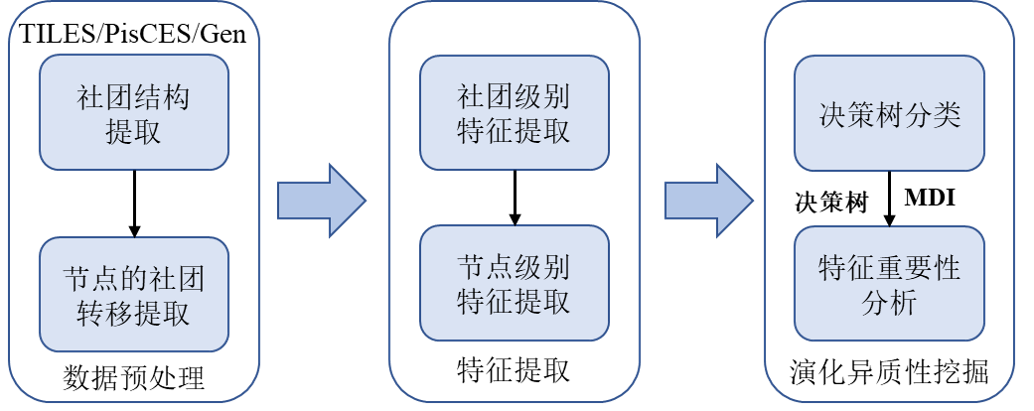
\includegraphics[width=.8\textwidth]{figures/chap03/figure/modelChap3.png}
	\caption{节点社团转移异质性探究方法流程图}
	\label{fig.3.1}
\end{figure}

动态网络演化的核心是节点在时序过程中的社团归属转移,而影响节点社团转移的因素则为动态网络生成与演化的高阶机理,因此需要探究影响节点社团转移的高阶因素,这里也称为节点的社团转移异质性因素。针对节点社团转移异质性的探究方法如图\ref{fig.3.1}所示,主要分为以下几个步骤:

\begin{enumerate}
\item 动态网络中的社团划分与节点的社团归属变迁分析。本研究首先采用成熟的动态网络社团识别技术,对每一时间快照下的网络社团结构进行解析。为避免单一算法可能引入的偏差,本部分选取三种不同的社团探测方法分别实施,包括GenLouvain算法\cite{GenLouvain}、PisCES方法\cite{PisCes}以及TILES算法\cite{rossetti2017tiles}。为确保动态网络快照划分的一致性,本研究将原始数据格式为$(源节点,目标节点,时间戳)$的动态网络(常见于公开数据集)转化为时间序列形式的网络切片结构,表示为$W={W^1, W^2, \dots, W^T}$,其中$T$代表时间片总数,$W^t \in {0,1}^{N \times N}$则为第$t$时刻的邻接矩阵。通过将相邻快照的节点与社团进行分组,形成多组连续快照网络,并将节点划分为社团不变与社团改变的两组节点,作为后续分类的标签。

\item 节点及社团层面的结构属性提取。本研究基于特征工程的理论基础并参考已有文献的经验性成果\cite{ilhan2016feature},设计并提取了两类共十个结构特征:其一为反映社团整体特性的五个宏观指标,用于探讨社团对节点行为的潜在影响;其二为描述节点个体属性的五个微观指标。具体而言,社团层面特征包括社团规模(节点数量)、社团活跃程度、社团连边数、内部边数、外部边数;节点层面特征则涵盖接近中心性、介数中心性、节点的社团传导性、节点度、邻居平均度。详细定义参见表\ref{fig.3.1}。特征提取的具体流程通过相邻时间片组实现,算法细节见算法\ref{chap3:alg1}。

\item 节点社团变迁的异质性探究。本部分采用决策树模型对节点社团归属变更标签进行分类。在分类完成后,通过计算平均不纯度降低(Mean Decrease in Impurity,MDI)指标,评估各特征在分类任务中的贡献度,从而量化不同结构属性在节点社团变迁过程中的相对重要性。这一分析结果进一步为揭示驱动节点社团归属异质性的深层机制提供了依据。
\end{enumerate}

\begin{algorithm}[!htbp]
	\caption{特征提取}
	\label{chap3:alg1}
	\algorithmicrequire \quad 无向图序列 $W = {W}^1,..{W}^T$ 和社团标签 $\mathcal{C} = \mathcal{C}^1,...\mathcal{C}^T$\\
	\algorithmicensure \quad 分类特征$F$ 和分类标签$L$
	\begin{algorithmic}[1]
		\FOR{图${W}^t$, $t \neq T$}
		\FOR{在$\mathcal{C}^t$的社团 $\mathcal{C}_l^t$  }
		\STATE 统计社团的特征$F_c$
		\FOR{$\mathcal{C}_l^t$中的节点$i$}
		\STATE 计算节点的相关特征$F_n$
		\STATE 组成分类$i$特征序列$F = F_c \vert F_n$
		\IF{$i$的社团标签发生变化}
		\STATE $i$的分类标签$L_i$ = 1
		\ELSE
		\STATE $i$的分类标签$L_i$ = 0
		\ENDIF
		\ENDFOR
		\ENDFOR
		\ENDFOR
	\end{algorithmic}
\end{algorithm}

% \end{enumerate}
在本研究框架的第一阶段,采用了三种已有的社团识别技术,即GenLouvain、PisCES和TILES,以实现动态网络中社团结构的解析。以下为对这三种方法的具体阐述:

1、GenLouvain是一种基于模块度优化的递归型社团探测算法,其核心目标是通过最大化模块度得分来划分网络社团。该方法通过迭代遍历网络节点对快照网络的社团结构进行识别,并引入了一种创新机制:将同一社团内的节点合并为超节点,从而实现网络结构的粗粒化处理。这种策略使其能够生成多层次的社团划分结果,因而特别适用于处理大规模网络的社团探测任务。

2、PisCES将谱聚类技术扩展至动态网络环境,通过综合分析时间维度信息与网络拓扑特性,追求全局最优的社团划分。该方法首先对所有网络快照的邻接矩阵执行特征分解,提取其特征向量并应用聚类算法(如k-means)进行初步分组。随后,通过引入时间平滑性约束,进一步优化聚类结果,确保社团划分在时间序列上的一致性,从而实现全局优化的社团识别。

3、TILES是一种基于标签传播的社团发现方法,能够识别动态网络中的重叠社团结构,并能够自动划分网络快照,为了保持网络结构一致性,本研究基于TILES所划分的快照进行探究。本研究假设,当某一节点在相邻快照中的社团归属发生显著变化时,可判定该节点经历了社团归属的变迁行为。
%\end{enumerate}




在特征提取阶段,本研究探讨了节点与社团两个层级结构在社团演化中的交互影响。研究认为,节点的行为不仅受自身属性驱动,其所属社团的特性同样可能对其行为产生作用,反之亦然。因此,为全面捕捉这种双向关系,本研究也提取了$6$个社团级别的特征来衡量社团对节点演化的影响力。针对节点演化异质性挖掘所构建的节点局部特征如表~\ref{tab.3.1}所示,其中$n$表示节点数,$e$表示边数,$l$表示社团编号,$t$表示快照编号(时间),$a$表示社团内活跃节点数,$C$表示社团内所有节点的集合,$\sigma_{jk}(i)$表示节点$j,k$之间的最短路径经过节点$i$的数量,$\sigma_{jk}$则表示节点$j,k$之间的所有最短路径。其中节点的度、平均邻居度、接近中心性以及介数中心性可以有效衡量节点在网络中的不同重要程度,而社团级别的特征也可以较全面地衡量社团在网络中的特征。

\begin{table}[!htbp]
	
	\centering
	\caption{节点局部特征的定义和符号表示}\label{tab.3.1}
	\vspace{0.5em}\centering\wuhao
	\begin{tabular}{lll}
		% \begin{tabular}{|l|l|l|l|}
			\hline
			符号&节点局部特征名 & 定义\\
			\hline
			$f1$&社团节点数  & $n_l^t$\\
			$f2$&社团边数 & $e_l^t$\\
			$f3$&社团内的边数 & $\frac{e_l^t(in)}{n_l^t}$\\
			$f4$&社团间的边数&  $\frac{e_l^t(out)}{n_l^t}$\\
			$f5$&社团活跃度 & $\frac{a_l^t}{n_l^t}$\\
			$f6$&社团连通率 &  $\frac{e_l^t}{d_l^t}$\\
			$f7$&节点的度 & $e_i^t$ \\
			$f8$&节点的平均邻居度 &  $\frac{1}{|N(i)^t|}\sum_{j\in N(i)^t}e_j^t$ \\
			$f9$&节点的接近中心性 &  $\sum_{j\in C_{l,-i}^t}\frac{C_l^t}{d(i,j)}$ \\
			$f10$&节点的介数中心性 &  $\sum_{j,k \in C_{l,-i}^t}\frac{\sigma_{jk}(i)}{\sigma_{jk}}$\\
			\hline
		\end{tabular}
		
	\end{table}


在特征重要性评估环节,本研究选用决策树作为节点归属变迁的二分类预测工具。相较于深度神经网络等黑箱模型,决策树因其透明性(即白箱特性)而更具优势,能够直观揭示每个特征在分类过程中的贡献。本研究最终采用平均不纯度降低(Mean Decrease in Impurity,MDI)方法\cite{menze2009comparison}量化各特征的重要性。MDI方法能够在决策树中给出各节点对最终分类的影响力大小,且计算效率较高,能够满足本研究的需求。
% ,其计算公式定义如下:

% \begin{equation}
% \centering
% \Delta i(s,r) = i(r) - p_L i(r_L) - p_R i(r_R)
% \end{equation}

% 其中,$i(r)$表示某一不纯度指标(如基尼指数),$r$为决策树中的某个分裂节点,$r_L$和$r_R$分别代表其左、右子节点。比例系数$p_L = N_{r_L}/N_r$表示左子节点的数据量占父节点数据量$N_r$的比例,类似地,$p_R = N_{r_R}/N_r$。通过标准化处理后的$\Delta i(s,r)$,可为每个特征生成一个重要性得分。此方法计算效率高,适用于大规模数据集的分析需求。









\subsection{用于网络高阶生成机理挖掘的数据描述}

% 本章所用数据集包括Internet、Facebook、Digg、Wikipedia等共$15$个不同类型的公开动态网络数据集以尽可能覆盖大部分常见的网络类型,对于数据集的详细描述见表\ref{tab.3.2}。如图\ref{fig.3.2}所示,用于研究的所有数据集均符合重尾分布,且同一来源的不同主题数据之间的度分布也存在偏差,这一定意义上证了本研究对真实世界数据挖掘任务的覆盖面。

本章研究所采用的数据集涵盖了Internet、Facebook、Digg、Wikipedia等在内的共15个公开动态网络数据集,旨在尽可能囊括多种常见的网络类型。有关各数据集的具体信息,可参见表\ref{tab.3.2}中的详细说明。本节所用数据集均不包含节点或边的属性信息,旨在从拓扑的角度总结与归纳影响节点社团演化的核心特征。


\begin{table}[!htbp]
	\centering
	\caption{用于网络高阶生成机理挖掘的数据集描述}\label{tab.3.2}
        \vspace{0.5em}\centering\wuhao
	\resizebox{\textwidth}{!}{
		\begin{tabular}{p{70pt}p{200pt}p{55pt}p{40pt}}
			\hline
			数据集&数据内容 & 节点数$|\mathcal{V}|$ & 边数$|\mathcal{E}|$\\
			\hline
			ia-digg-reply &Digg社交网站网络\cite{nr},时间跨度为2008年10月29日至2008年11月13日 & $30397$ & $87627$\\
			ia-facebook-wall-wosn-dir & Facebook关注与被关注网络\cite{nr},时间跨度2004年5月15日至2004年10月24日 & $44668$ & $876993$\\
			ia-reality-call & MIT的手机接打电话网络\cite{nr},时间跨度为 2004年9月24日-2005年10月7日& $6810$ & $52050$\\
			ia-slashdot-reply-dir & Slashdot\cite{nr}网站的问答网络,时间跨度为2005年12月7日-2006年8月31日 & $51097$ & $140778$\\
			ia-stackexch-user-marks-post & StackOverflow\cite{nr}的问答网络,时间跨度为2008年10月3日-2011年11月25日 & $545196$ & $1302439$\\
			ia-yahoo-messages & 雅虎\cite{nr}的消息网络,时间跨度未知& $99303$& $3179718$\\
			soc-epinions-trust-dir & Epinion的关联网络\cite{nr},时间跨度未知& $131828$ & $841373$\\
			soc-wiki-elec & Wikipedia的页面投票网络\cite{nr},时间跨度2004年9月14日-2008年1月5日 & $8271$ & $107071$\\
			wiki& Wikipedia网页关联网络\cite{mislove-2009-socialnetworksthesis},时间跨度2001年2月20日-2002年12月6日 & $329623$ &$39953145$\\
			Internet & 因特网\cite{mislove-2009-socialnetworksthesis}数据,时间跨度2004年1月4日 -2005年4月4日& $33936$ & $104824$\\
			Facebook & 脸书在新奥尔良地区的交友网络\cite{viswanath-2009-activity} ,时间跨度 2008年8月6日-2009年1月21日&$62306$& $905565$\\
			bitcoin & 比特币\cite{kumar2016edge}的信任链网络,时间跨度2010年11月9日-2016年1月19日 & $5881$ & $35592$\\
			Friend & 美国某社区的现实世界交友网络\cite{aharony2011social},时间跨度2010年7月10日-2011年7月16日 & $130$ & $60518$\\
			fb-forum & 脸书某论坛帖子网络\cite{nr},时间跨度2004年5月15日-2004年10月24日 & $899$ & $33720$\\
			fb-messages & 脸书加州学生社区的消息网络\cite{nr},时间跨度2004年3月 24日-2004年10月22日 & $1897$ & $61734$\\

			\hline
		\end{tabular}
	}
\end{table}


% \begin{figure}[!htbp]
% 	\setlength{\abovecaptionskip}{0pt} 
% 	\setlength{\belowcaptionskip}{10pt} 
% 	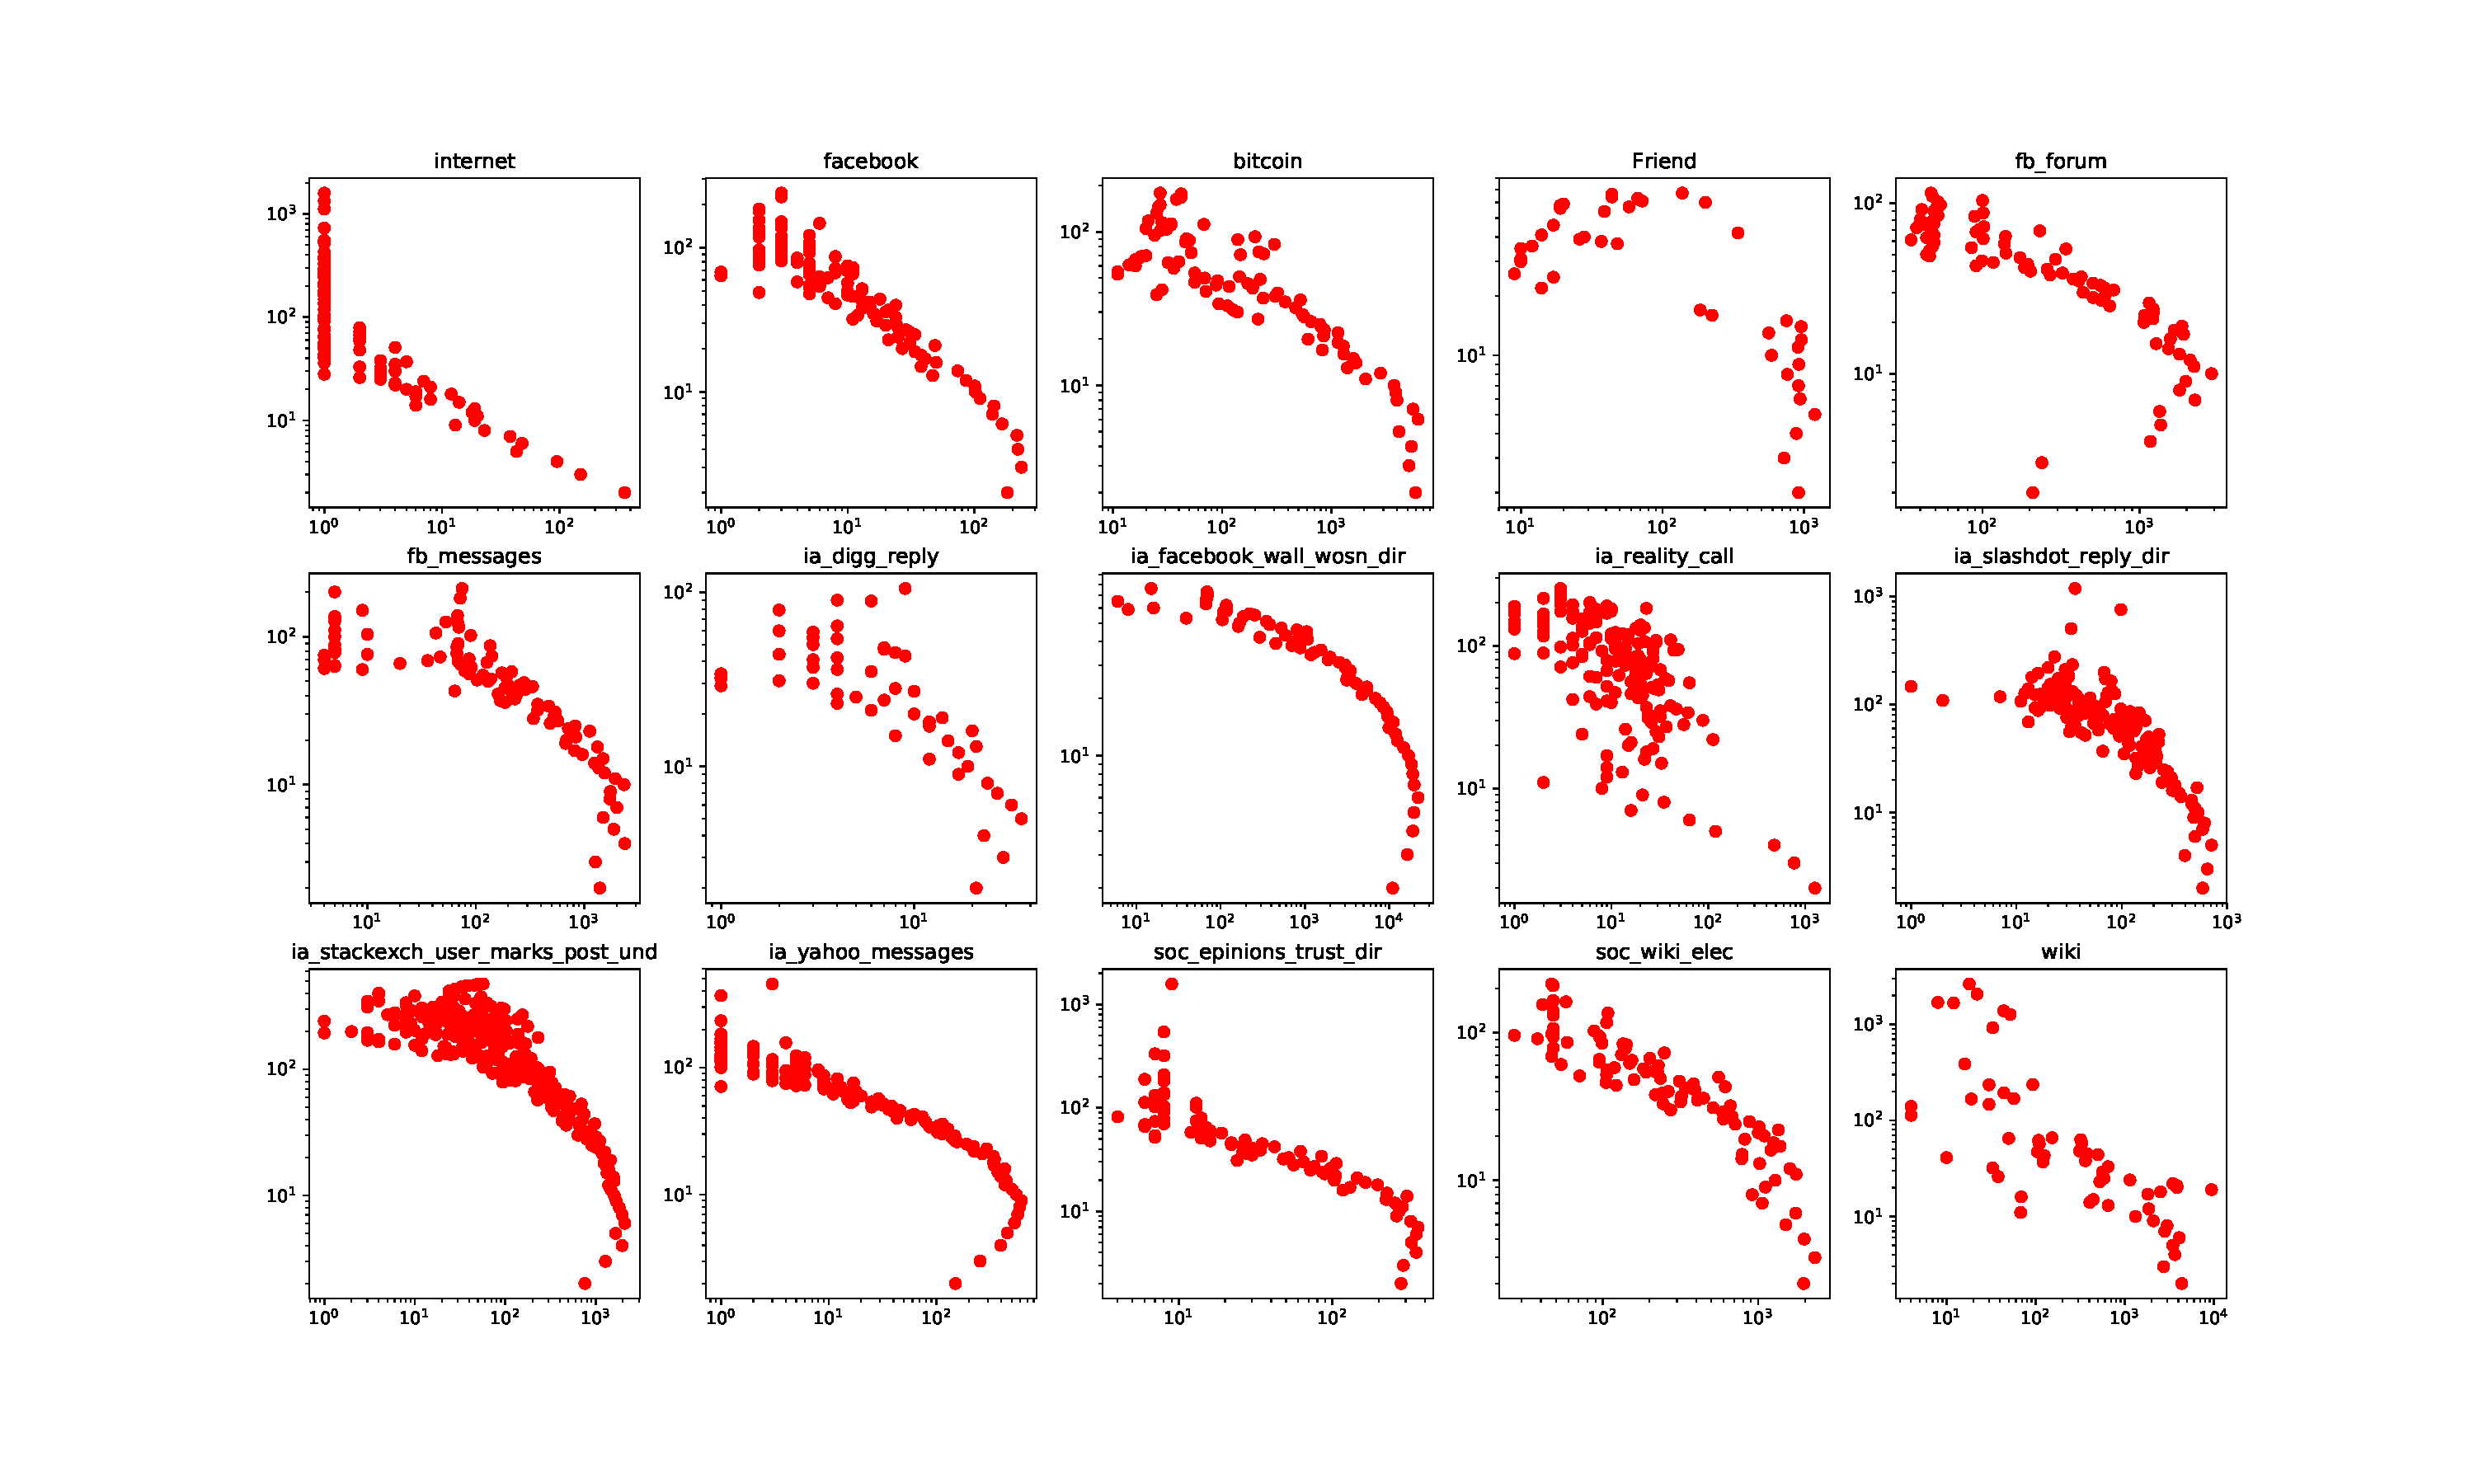
\includegraphics[width=.9\textwidth]{figures/chap03/figure/degrees.pdf}
% 	\caption{15个真实数据集的度分布可视化}
% 	\label{fig.3.2}
% \end{figure}

\subsection{节点演化异质性归纳}

% \subsubsection{实验及结论}

% 按照上文所述的研究框架处理上述$15$个数据集,并计算其特征重要性。结果如图\ref{fig.3.3}所示,图中横坐标表示节点如表\ref{fig.3.1}所述的分类特征;纵坐标分别表示$15$个数据集,颜色代表特征在不同数据集中的分类任务中所占重要性,颜色越浅表示该特征重要性越高。可以看到$f7$(节点的度)与$f8$(节点的平均邻居度)在所有特征分类中均占很大比重,尤其在$fb-forum$数据中,节点的平均邻居度在分类中所占比重超过了$0.5$;而$f5$(社团活跃度)在$ia-slashdot-reply-dir$数据中所占比重超过其他数据,该数据为技术网站Slashdot的回复网络,从这一点来看,\textbf{科技类网站的圈子活跃度}是影响其用户更换兴趣圈的主要因素;与此同时,在$internet$网络中,$f9$(节点的接近中心性)对其节点的社团转移影响最大,显而易见,在因特网中,连通性是其最至关重要的指标之一。虽然$f5,f9$均在某些数据集中显示出了对节点社团转移的重要影响力,但是其并不具有普遍性。反观$f7,f8$,其在所有数据集中对节点的社团转移均具有可观的影响力。因此本研究可得出初步结论,\textbf{节点的度以及节点的平均邻居度是影响节点发生社团转移的重要的结构特征}。进一步可以确定,节点的社团转移存在异质性,即\textbf{社团内不同的节点具有不同的转移倾向性}。

% 另外,为了去除社团检测算法偏差,本研究基于GenLouvain和PisCES两个社团检测算法的结果如图~\ref{fig.3.3Gen}和图~\ref{fig.3.3Pis}所示,其结果也证实了本研究的结论,即社团内不同节点具有不同的转移倾向,但细节方面存在一定偏差,如节点级特征$f9,f10$在GenLouvain方法中具有更大的占比,而在PisCES中$f7$节点的度在$ia_reality_call$数据集中相较于另外两个社团检测方法具有更高的重要性。
通过对上述数据集的挖掘,结果如图~\ref{fig.3.3}所示。热图中横坐标代表特征编号,纵坐标代表数据集,颜色越浅表示分类特征重要性越高。可以看到,去除社团检测算法差异后,节点级别的特征在社团转移过程中占有较高的重要性,其中以节点的平均邻居度和节点的度对分类影响最大,即动态网络中,社团内不同的节点具有不同的社团转移倾向性,且单独的某一个特征并不能决定节点的社团转移。这也证明了在动态网络生成过程中,节点的高阶特征如平均邻居度对网络及社团演化具有显著的影响,这为后续模型对动态网络生成模式的建模提供了实证依据。


\begin{figure}[!htbp]
        \subfigure[基于TILES]{
        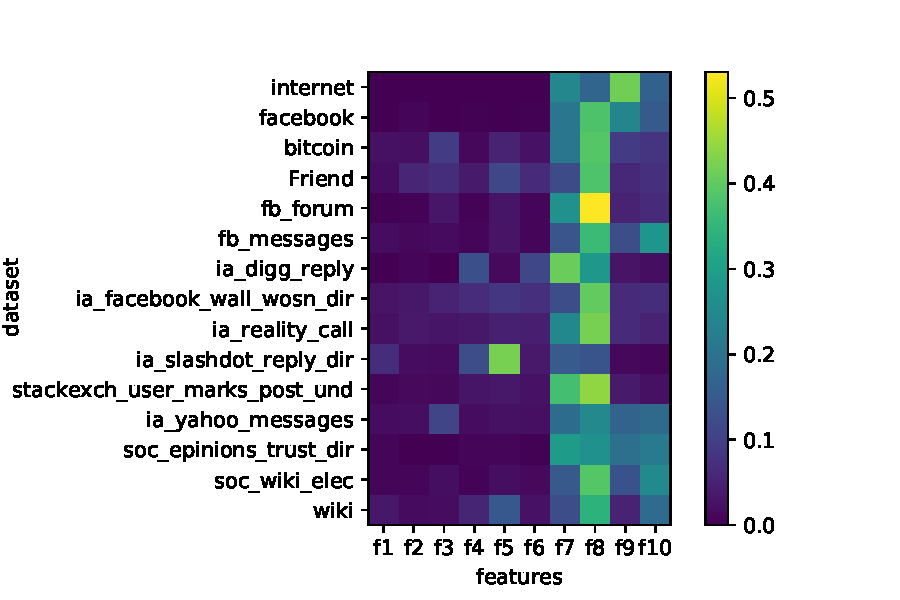
\includegraphics[width=.31\textwidth]{figures/chap03/figure/15cmp.pdf}
        }
	\subfigure[基于GenLouvain]{
    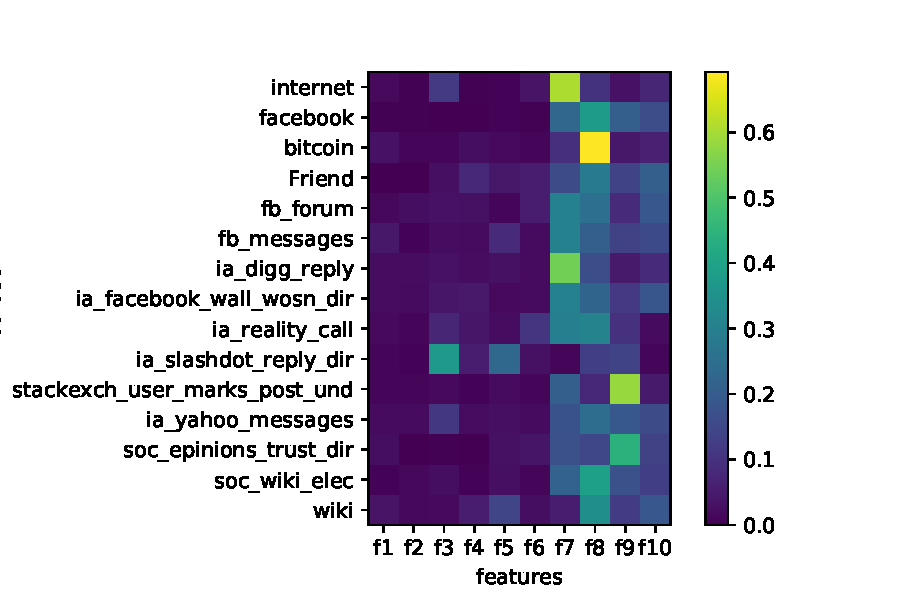
\includegraphics[width=.31\textwidth]{figures/chap03/figure/resultGenlou.pdf}
        }
        \subfigure[基于PisCES]{
    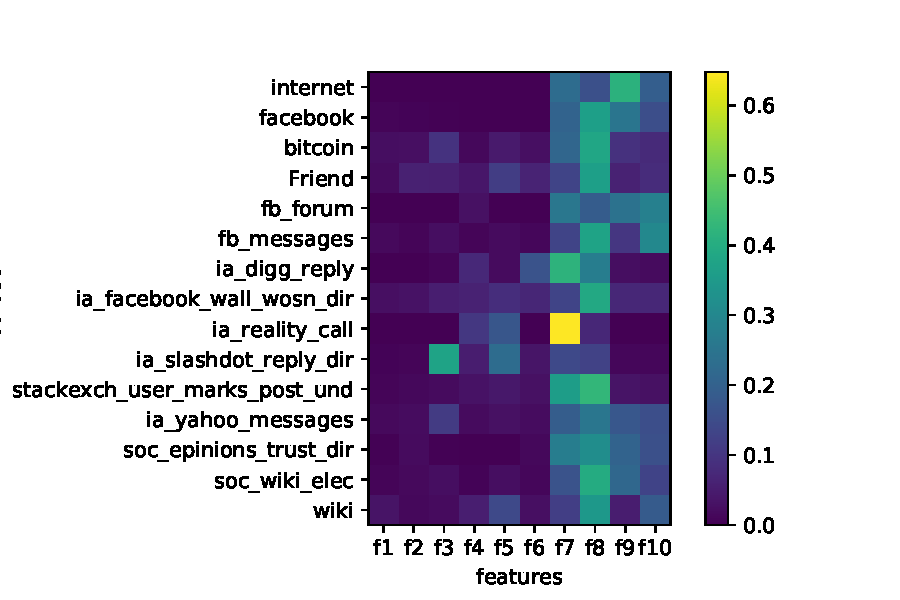
\includegraphics[width=.31\textwidth]{figures/chap03/figure/resultPNAS15.pdf}
        }
	\caption{基于不同社团检测算法的$15$个数据集的特征重要性热图}
	\label{fig.3.3}
\end{figure}

为了从定量的角度探究节点的度与平均邻居度如何影响节点的社团转移,本节还绘制了二者在所有数据集中发生与未发生社团转移的数据分位图。如图~\ref{fig.3.4}与图~\ref{fig.3.5}所示,其中横坐标为$1$表示发生节点转移,横坐标为$0$表示未发生节点社团转移,可以看到节点的度越小,节点越可能受到邻居影响而发生社团转移;反之节点的平均邻居度越大,越可能发生社团转移,但各数据集的噪声过多且模式并不清晰,因此难以得到定量的结论。但仍然能够定性地确定节点在社团演化中存在异质性,且与节点及其邻居的重要性直接相关。
% 为了探究节点的度以及节点的平均邻居度是以何种模式影响节点的社团转移的,本文分别统计了以上两个节点结构属性在$15$个数据集中的分布。如图\ref{fig.3.4}所示,该图展示了节点的度在十五个数据集中的分位图,每个子图中共有两列分位图,分别为发生转移的节点(横坐标为$1$)以及未发生转移的节点(横坐标为$0$)的度的分位统计图。从图中可以看到,在所有$15$个数据集中,发生社团转移的节点的度普遍比未发生转移的节点的度更高,即在一个网络中,节点的度越高,其越有可能发生社团转移。这也验证了社团检测中的大量度修正方法~\cite{wilson2016modeling,jin2015modeling}的正确性。而图\ref{fig.3.5}则展示了节点的平均邻居度在十五个数据集中的分位图,每个子图中共有两列分位图,分别为发生转移的节点(横坐标为$1$)以及未发生转移的节点(横坐标为$0$)的平均邻居度的分位统计图。可以看到节点的平均邻居度在不同数据集中的发生转移以及未发生转移节点中的值并不相同,这说明不同的节点平均邻居度确实在影响节点的社团转移行为,然而其模式在所有十五个数据集中并不统一。

 \begin{figure}[!htbp]
 	\centering
 	\setlength{\abovecaptionskip}{0pt} 
 	\setlength{\belowcaptionskip}{10pt} 
 	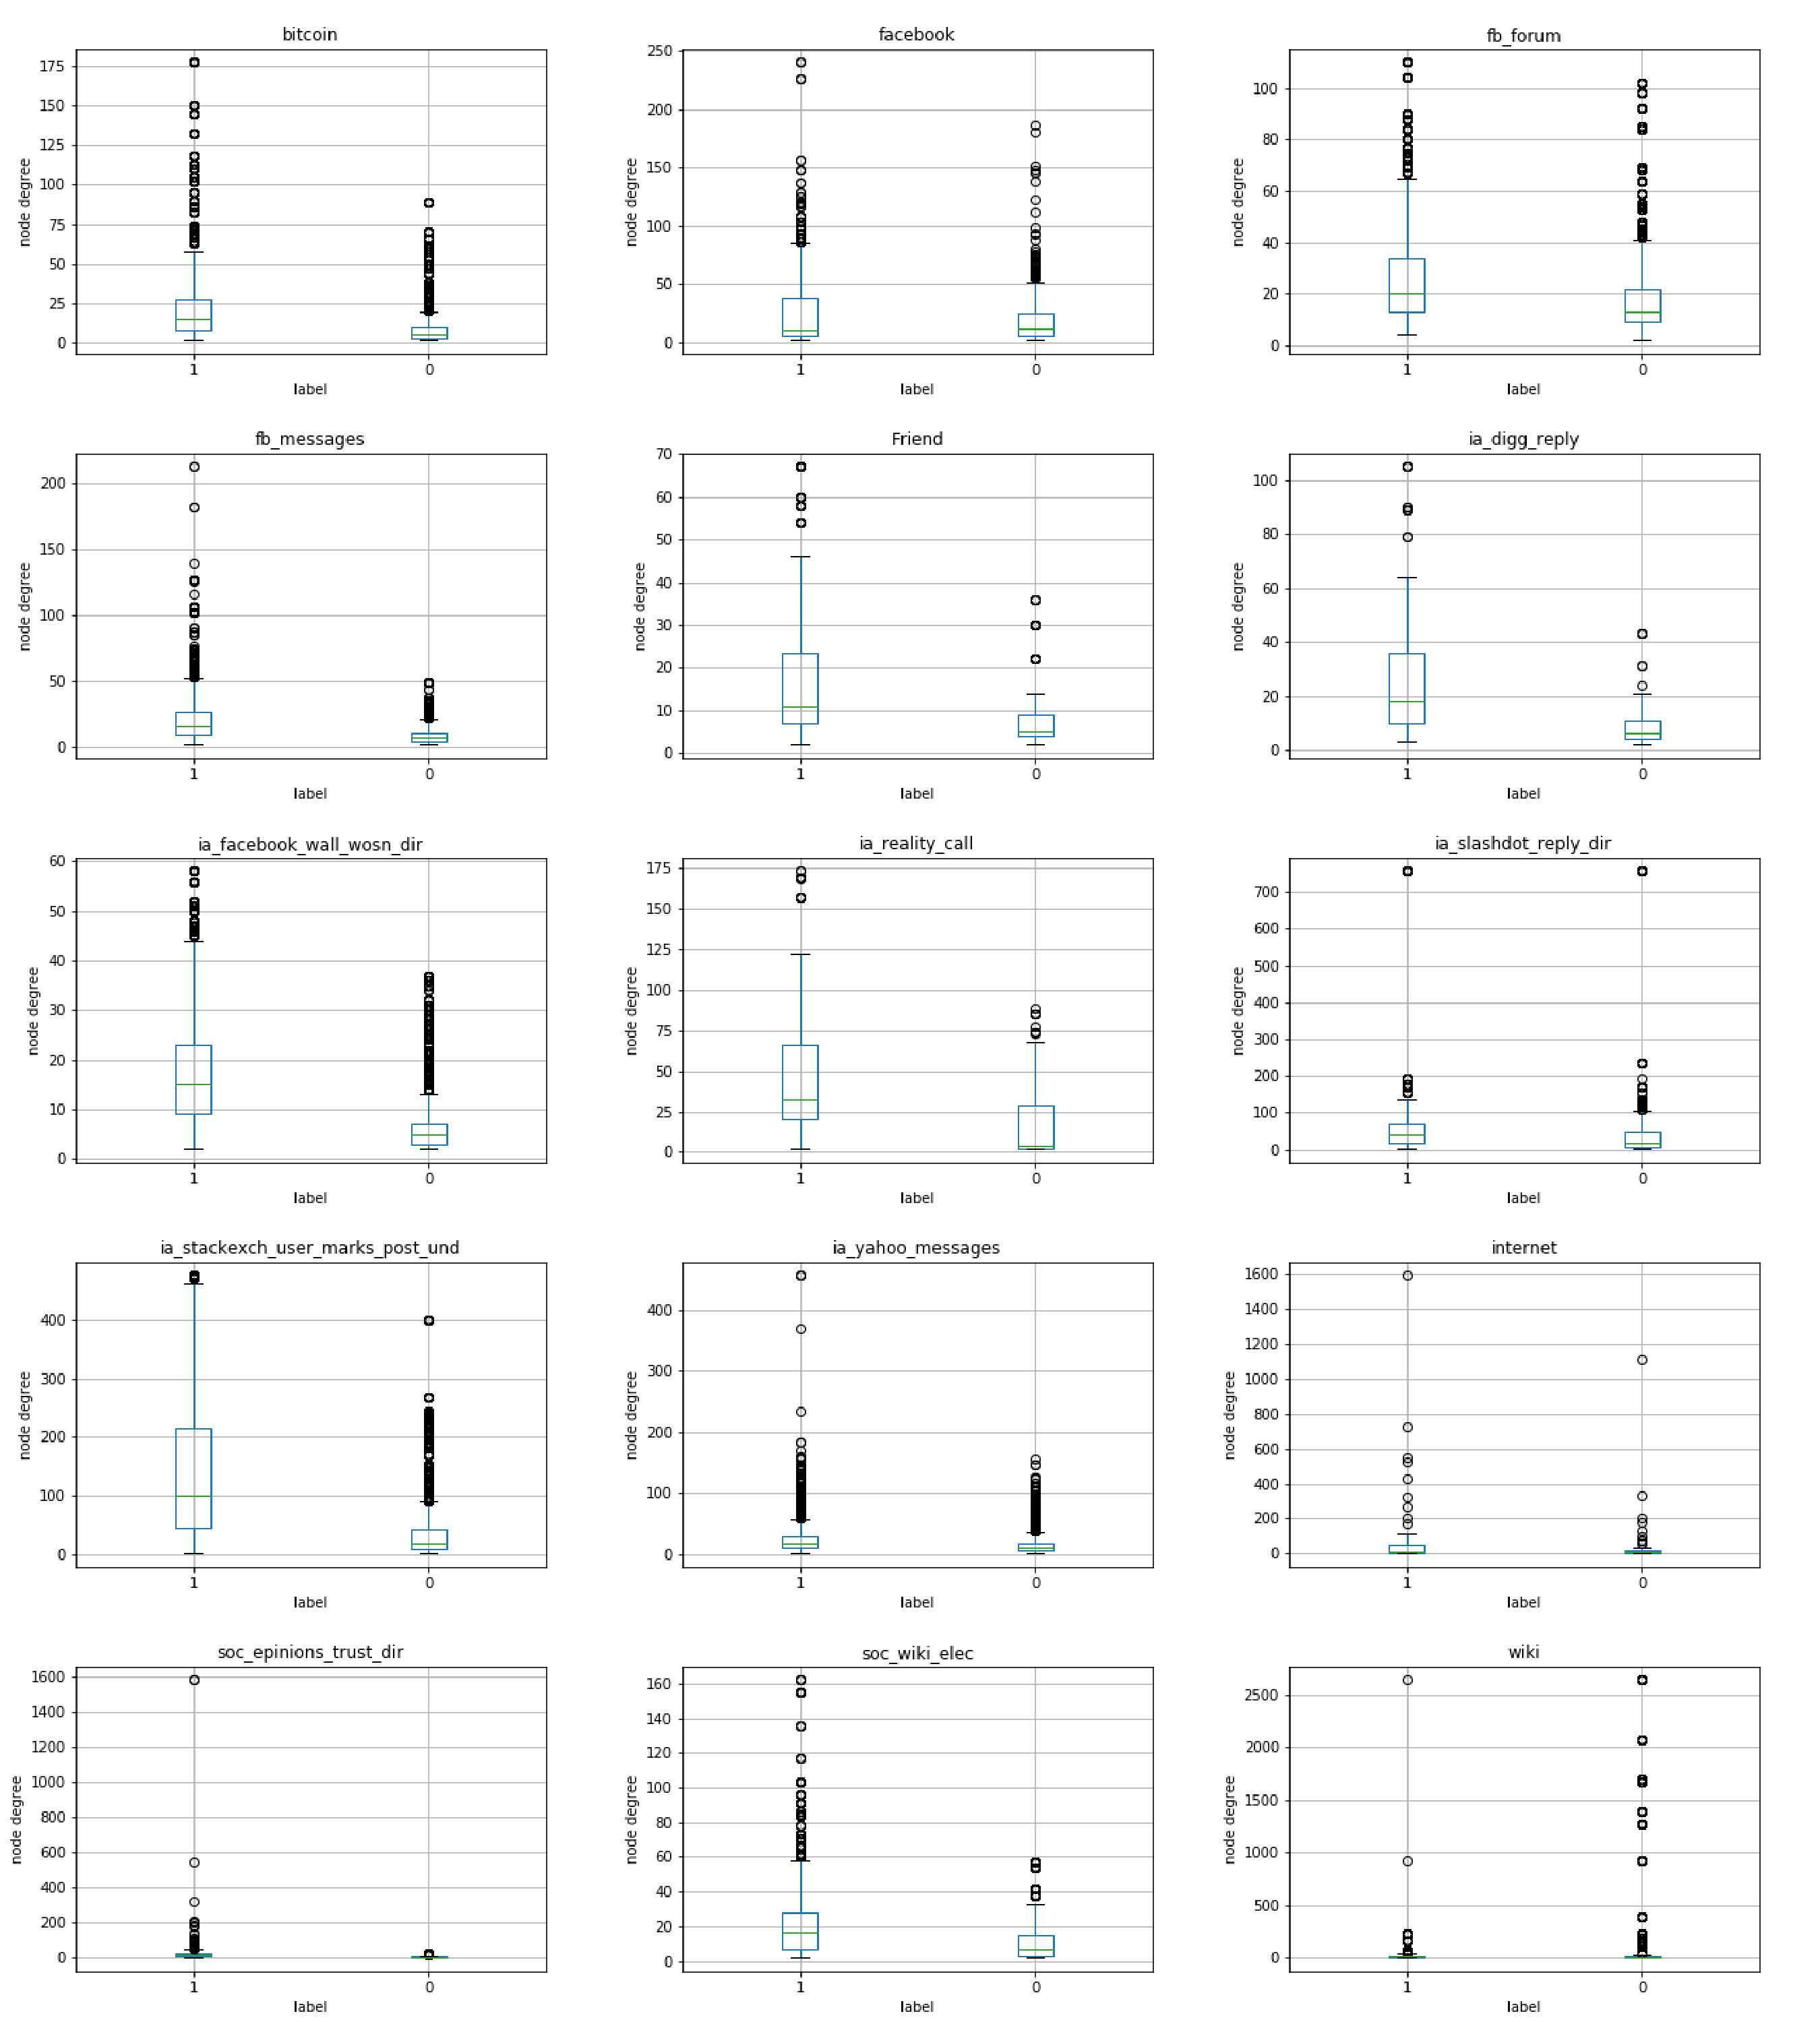
\includegraphics[width=.6\textwidth]{figures/chap03/figure/alldata-DG.pdf}
 	\caption{15个数据集的节点度的分位图}
 	\label{fig.3.4}
 \end{figure}

 \begin{figure}[!htbp]
 	\centering
 	\setlength{\abovecaptionskip}{0pt} 
 	\setlength{\belowcaptionskip}{10pt} 
 	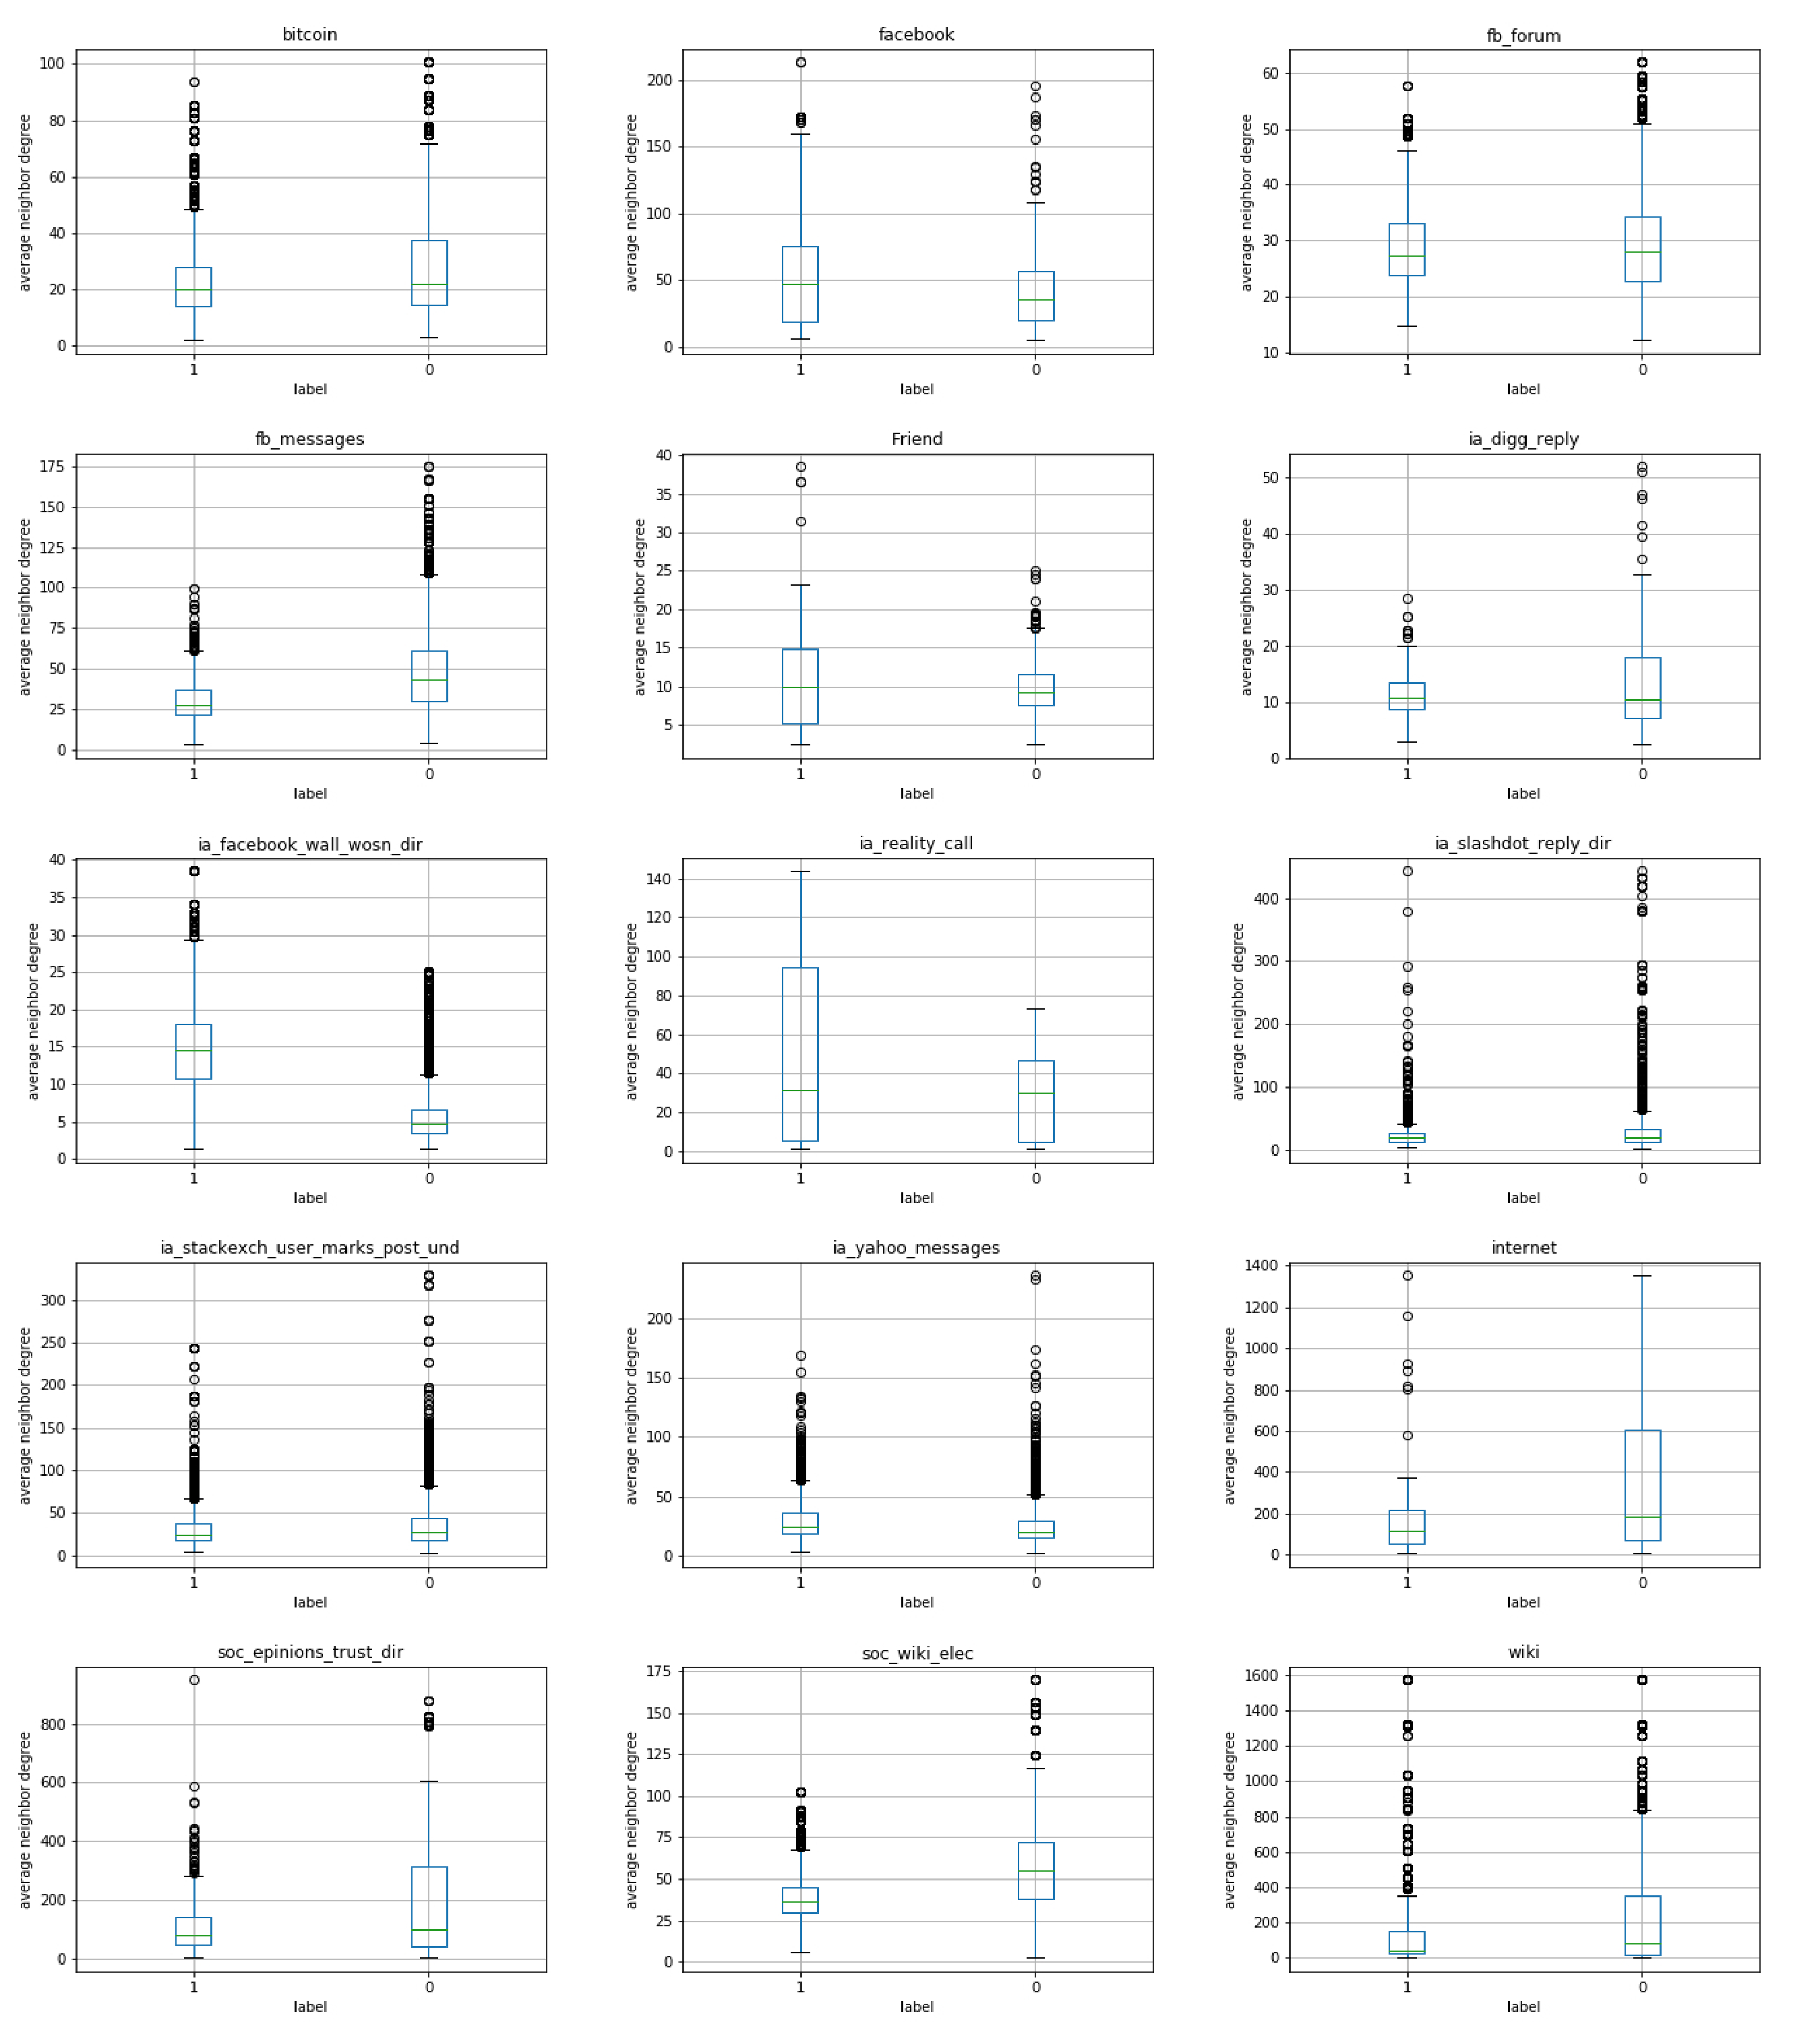
\includegraphics[width=.6\textwidth]{figures/chap03/figure/alldata-aND.pdf}
 	\caption{15个数据集的节点的平均邻居度的分位图}
 	\label{fig.3.5}
 \end{figure}



\section{融合节点社团转移异质性的动态随机块模型}
上述研究从实际数据集的角度证明了节点在动态网络中社团转移异质性的存在,受此启发,本文提出了基于动态随机块模型DSBM的层次贝叶斯动态随机块模型HB-DSBM。

\subsection{HB-DSBM的准备工作}


% 在介绍模型前,本节首先介绍模型的符号表示。如表\ref{tab.4.1}所示,用$W=\{W^1,W^2,...,W^T\}$表示动态网络邻接矩阵,即$W^t$表示第$t$个网络快照的邻接矩阵,其中$t \in 1,...,T$。这里$W^t \in \{0,1\}^{N\times N}$,$W_{ij}^t = 0$则代表$i$节点与$j$节点在网络快照$t$中没有边,若为$1$则有边。这里为了方便叙述,本章认为网络是无向无权的,这里需要说明,HB-DSBM可以有效的扩展为有向有权网络。$Z = \{Z^1,Z^2,...,Z^T\}$代表每个网络快照中节点的社团划分,例如$z_i^t = k$则表示$i$节点在网络快照$t$中属于$k$社团,其中$k\in K$。

在正式介绍模型之前,本节首先阐释本章的符号体系。如附录A.1~表\ref{symbols:all}所示,动态网络的邻接矩阵集合用$W={W^1, W^2, \dots, W^T}$表示,其中$W^t$对应第$t$个网络快照的邻接矩阵,$t$取值范围为$1$至$T$。本章中,$W^t \in {0,1}^{N \times N}$,$W_{ij}^t = 0$表示在快照$t$中节点$i$与节点$j$之间不存在边,而$W_{ij}^t = 1$反之。为了方便描述,本章假设输入的网络是无向且无权的。对于无向无权网络,可以通过设置邻接矩阵非对称或邻接矩阵的数值为大于等于$0$的整数,并将连边分布设置为泊松分布进行适配。$Z = {Z^1, Z^2, \dots, Z^T}$则表示动态网络每个快照的社团划分,当$z_i^t = k$时,表示节点$i$在$t$时刻属于社团$k$,$k \in K$,$z_i$也可以用one-hot向量进行表示。

\subsection{HB-DSBM的模型设计}

\begin{figure}[!htbp]
	\setlength{\abovecaptionskip}{0pt} 
	\setlength{\belowcaptionskip}{10pt} 
	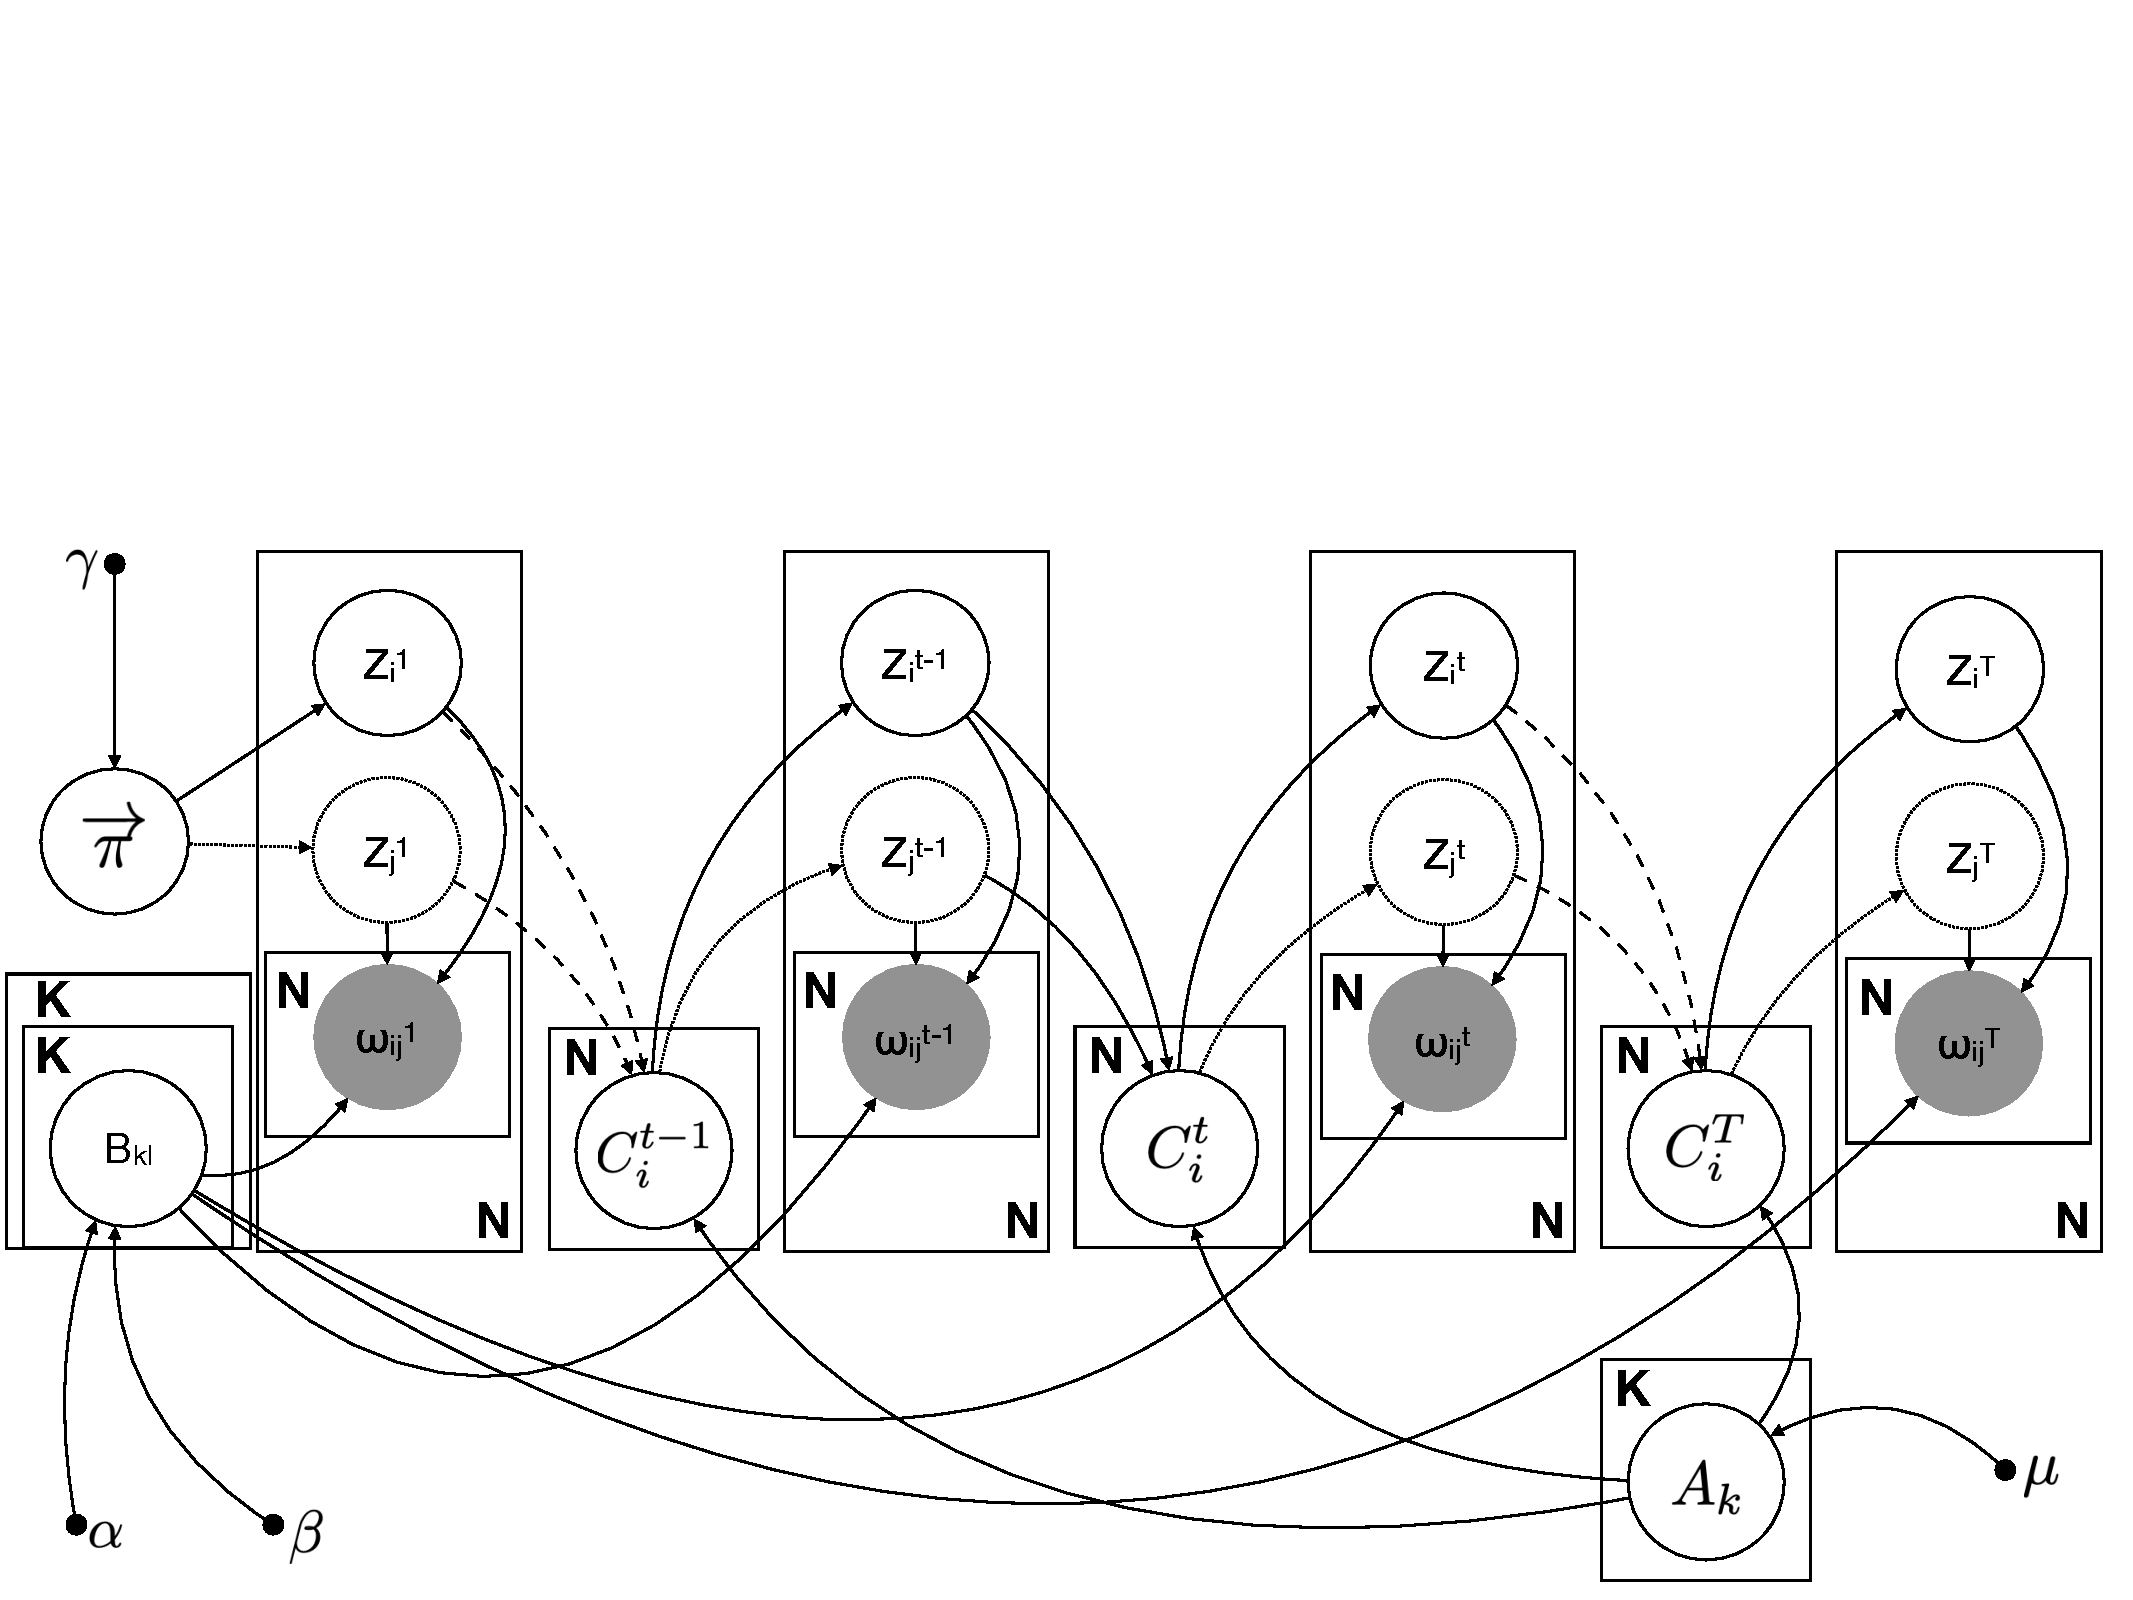
\includegraphics[width=.9\textwidth]{figures/chap04/graph-model_v3_cuted.pdf}
	\caption{HB-DSBM图模型}
	\label{fig.4.1}
\end{figure}

% 本节首先介绍HB-DSBM的核心生成机制来揭示它是如何通过层次贝叶斯结构同时建模社团级别和节点级别的动态演化的,随后给出其产生社团结构和动态网络的生成过程。

% 如图~\ref{fig.4.1}的图模型所示,HB-DSBM首先令$\pi$表示$Z^1$的先验分布,同时$\pi$服从参数为$\gamma$的狄利克雷分布。$B$是不同社团间节点的连边概率,即类随机块模型中的块矩阵,例如$B_{kl}$即代表属于$k$社团和属于$l$社团的节点之间连边的伯努利分布概率。而$B$服从参数为$\alpha$和$\beta$的Beta分布。

% 本章中的$A \in [0, 1]^{K \times K}$表示社团级别转移倾向矩阵,$A$的每一行$A_k$都服从参数为$\mu$的狄利克雷分布,因此 $\sum_l A_{kl} = 1$。同时$C = \{ C^2, \cdots C^T \}$表示节点级别的社团转移倾向,每个$C^t$都是由社团级别转移倾向矩阵$A$生成。对于$t>1$的网络快照,任意节点$i$都有其唯一的转移向量 $C_i^t  \in [0, 1]^K$,该向量服从以参数为$A_{z_i^{t-1}}$的狄利克雷分布,因此$\sum_{k} C_{ik}^t = 1$。这一部分就是本模型的核心:层次狄利克雷生成机制。

% 基于以上机制,模型可以生成社团标签以及动态网络中每个网络快照中的边。具体生成过程如下所示:
% \begin{enumerate}
% 	\item 生成初始社团划分概率 ${\pi} \sim Dir({\gamma})$
% 	\item 生成块矩阵 $B \sim Beta({\alpha},{\beta})$
% 	\item 对于网络快照$t=1$的每个节点$i$:
% 	\begin{enumerate}
% 		\item 生成每个节点的社团归属 $z_i^1 \sim Mult({\pi})$ 
% 		\item 生成每条边 $\omega_{ij}^1 \sim Bernoulli(\cdot | B_{z_i^1,z_j^1})$
% 	\end{enumerate}
% 	\item 生成每个社团级别转移矩阵的社团转移向量 ${A}_k \sim Dir({\mu})$
% 	\item 对网络快照$t>1$中的每个节点$i$:
% 	\begin{enumerate}
% 		\item 生成每个节点级别的社团转移向量${C}_i^t \sim Dir({A}_{z_i^{t-1}})$
% 		\item 生成每个节点的社团归属 $z_i^t \sim Mult({C}_i^t)$
% 		\item 生成每条边 $\omega_{ij}^t \sim Bernoulli(\cdot | B_{z_i^t,z_j^t})$
% 	\end{enumerate}
% \end{enumerate}



首先介绍本方法的生成机制,详细介绍所设计的层次狄利克雷生成结构如何生成节点级别的社团转移倾向矩阵,然后介绍整个网络的生成过程。


如图~\ref{fig.4.1}所示,首先$Z^1$的先验分布为以$\pi$为参数的分类分布,而$\pi$则服从以$\gamma$参数的Dirchlet分布。$B$表示动态随机块中的连边概率,即块矩阵,其服从以$\alpha$和$\beta$为参数的Beta分布。

$A \in [0, 1]^{K \times K}$表示社团级别的转移倾向矩阵,$A_k$服从以$\mu$为参数的Dirchlet分布,并满足$\sum_l A_{kl} = 1$。$C = { C^2, \dots, C^T }$则表示节点的社团转移倾向,$C^t$由$A$进行生成。当$t>1$时,节点$i$的社团转移倾向为$C_i^t \in [0, 1]^K$,服从以$A_{z_i^{t-1}}$为参数的Dirchlet分布,且$\sum_{k} C_{ik}^t = 1$。这一层次生成机制由Dirchlet分布构成,因此本文称之为层次狄利克雷生成结构,也是本模型对节点的演化异质性建模的核心。

综上所述,HB-DSBM的生成过程如下:
\begin{enumerate}
\item  生成$t=1$时的社团划分先验分布${\pi} \sim Dir({\gamma})$;
\item 生成块矩阵$B \sim Beta({\alpha}, {\beta})$;
\item 对$t=1$的节点$i$:
\begin{enumerate}
\item 生成初始社团划分$z_i^1 \sim Mult({\pi})$;
\item 生成边 $\omega_{ij}^1 \sim Bernoulli(\cdot | B_{z_i^1, z_j^1})$;
\end{enumerate}
\item 生成社团级别转移倾向矩阵${A}k \sim Dir({\mu})$;
\item 对$t>1$的每个节点$i$:
\begin{enumerate}
\item 生成节点异质性转移向量${C}i^t \sim Dir({A}{z_i^{t-1}})$;
\item 生成社团划分$z_i^t \sim Mult({C}i^t)$;
\item 生成边$\omega{ij}^t \sim Bernoulli(\cdot | B{z_i^t, z_j^t})$。
\end{enumerate}
\end{enumerate}


% 由生成过程可知,当$t=1$时,模型首先利用参数为$\pi$的多项分布生成$i$的社团归属$z_i^1$,随后以伯努利分布 $Bernoulli(\cdot|B_{z_i^1,z_j^1})$生成每对节点对$i,j$之间的连边。而当$t>1$时,$i$节点的社团归属由以参数为$C_i^t$的多项分布决定,即$z_i^t \sim Mult({C}_i^t)$。而$C_i^t$服从狄利克雷分布$Dir(A_{z_i^{t-1}})$。

% 根据如图~\ref{fig.4.1}的概率图模型和生成过程,可以写出HB-DSBM的联合概率分布如下:

% \begin{equation}
% \begin{split}
% Pr&(W_T,Z_T,C_T,B,A,\pi|\alpha,\beta,\gamma,\mu) \\
% = & \prod_{t=1}^T Pr(W^t | Z^t,B) Pr(Z^1|\pi) \prod_{t=2}^T Pr(Z^t|C^t) \\
% & \prod_{t=2}^T Pr(C^t|A,Z^{t-1}) Pr(A|\mu) Pr(\pi|\gamma) Pr(B|\alpha,\beta) \\
% \end{split}
% \end{equation}

从生成过程可以看出,当$t=1$时,模型首先通过以$\pi$为参数的多项分布生成节点$i$的社团归属$z_i^1$,随后利用伯努利分布$Bernoulli(\cdot|B_{z_i^1,z_j^1})$确定节点对$(i,j)$之间的连接关系。而对于$t>1$的情况,节点$i$的社团归属$z_i^t$由以$C_i^t$为参数的多项分布生成,即$z_i^t \sim Mult({C}_i^t)$,其中$C_i^t$则遵循以$A_{z_i^{t-1}}$为参数的狄利克雷分布$Dir(A_{z_i^{t-1}})$。

由图模型~\ref{fig.4.1}与HB-DSBM的生成过程可写出模型的联合概率分布:

\begin{equation}
\begin{split}
P&(W_T, Z_T, C_T, B, A, \pi | \alpha, \beta, \gamma, \mu) \\
= & \prod_{t=1}^T P(W^t | Z^t, B) \times  P(Z^1 | \pi) \times \prod_{t=2}^T P(Z^t | C^t) \\
& \times \prod_{t=2}^T P(C^t | A, Z^{t-1}) \times P(A | \mu) \times P(\pi | \gamma) \times P(B | \alpha, \beta) ,\\
\end{split}
\end{equation}


% \section{模型求解}

% 本小结介绍针对本模型的高效的变分近似推断算法。
% \subsection{变分推断}
% 由于模型参数较多且复杂,直接推出模型后验$p(Z,C,B,A,\pi|W)$是困难的, 因此基于平均场理论,本节提出了用$q(Z,C,B,A,\pi)$ 来近似$p(Z,C,B,A,\pi|W)$. 为了简介,本节用$\Delta$ 来表示参数 $\{\pi,B,A,C,Z\}$. 更详细来说,即:

% \begin{equation}
% \label{eq2}
% \begin{split}
% & q(\Delta) =  \prod_{t=1}^T \prod_{i=1}^N q(z_i^t) \prod_{t=2}^T \prod_{i=1}^N q(c_i^t)q(B)q(A)q(\pi)  \\
% \end{split}
% \end{equation}

% 其中块矩阵变分参数$q(B|\widetilde{\alpha},\widetilde{\beta}) = \prod_{k,l\geq k} Beta(\widetilde{\alpha}_{kl},\widetilde{\beta}_{kl})$, 社团级别转移矩阵变分参数 $q(A|\widetilde{\mu}) = \prod_{k=1}^K \prod_{l=1}^K Dir(\widetilde{\mu}_{kl})$。 而社团归属变分参数$q(z_i^t|\widetilde{\phi}_i^t)$ 服从以$\widetilde{\phi}_i^t$为参数的多项分布。
% 而$q(c_i^t|\widetilde{\xi}_i^t)$和$q(\pi|\widetilde{\gamma})$都分别服从以$\widetilde{\xi}_i^t$和$\widetilde{\mu}_{kl}$为参数的狄利克雷分布。

\section{HB-DSBM模型求解}
本节介绍基于变分推断的HB-DSBM参数后验求解方法,具体如下所述。

\subsection{HB-DSBM参数的近似后验推断}

模型后验分布$p(Z, C, B, A, \pi | W)$由于各分部并非共轭分部,因此难以直接推断。本研究基于平均场理论,提出基于变分推断理论,以$q(Z, C, B, A, \pi)$近似替代$p(Z, C, B, A, \pi | W)$。为简化表述,本节将参数集合$\{\pi, B, A, C, Z\}$统一记作$\Delta$。具体而言,变分分布的因子分解形式如下:

\begin{equation}
\label{eq2}
\begin{split}
& q(\Delta) = \prod_{t=1}^T \prod_{i=1}^N q(z_i^t) \cdot \prod_{t=2}^T \prod_{i=1}^N q(c_i^t) \cdot q(B) \cdot q(A) \cdot q(\pi) , \\
\end{split}
\end{equation}

其中,块矩阵的变分参数分布定义为$q(B | \widetilde{\alpha}, \widetilde{\beta}) = \prod_{k,l \geq k} Beta(\widetilde{\alpha}_{kl}, \widetilde{\beta}_{kl})$,社团层面转移矩阵的变分参数分布为$q(A | \widetilde{\mu}) = \prod_{k=1}^K \prod_{l=1}^K Dir(\widetilde{\mu}_{kl})$。节点社团归属的变分参数$q(z_i^t | \widetilde{\phi}_i^t)$遵循以$\widetilde{\phi}_i^t$为参数的多项分布。此外,节点级转移倾向的变分参数$q(c_i^t | \widetilde{\xi}_i^t)$和先验分布$q(\pi | \widetilde{\gamma})$分别服从以$\widetilde{\xi}_i^t$为分属以及以$\widetilde{\gamma}$为参数的Dirchlet分布。


% 因此有变分下界:

% \begin{equation}
% \label{eq:3}
% \begin{split}
% &\widetilde{L}(q) = \sum_z \int_{\pi,B,A,C}q(\Delta) \log \frac{p(\Delta,W)}{q(\Delta)} 
% = E_{\widetilde{\phi},\widetilde{\alpha},\widetilde{\beta}} \sum_{t=1}^T [\log P(W^t|Z^t,B)] \\
% &+ E_{\widetilde{\gamma},\widetilde{\phi}}[\log P(Z^1|\pi)]+E_{\widetilde{\phi},\widetilde{\xi}} \sum_{t=2}^T [\log P(Z^t|C^t)] 
% + E_{\widetilde{\xi},\widetilde{\phi},\widetilde{\mu}} \sum_{t=2}^T [\log P(C^t|A,Z^{t-1})]\\
% &+ E_{\widetilde{\mu}}[\log P(A)]+E_{\widetilde{\gamma}}[\log P(\pi)] + E_{\widetilde{\alpha},\widetilde{\beta}}[\log P(B)]
% - E_{\widetilde{\gamma}}[\log q(\pi)] - E_{\widetilde{\alpha},\widetilde{\beta}}[\log q(B)]  - E_{\widetilde{\mu}}[\log q(A)]\\
% &- \sum_{t=2}^T \sum_{i=1}^N E_{\widetilde{\xi}}[\log q(C_i^t)] - \sum_{t=1}^T \sum_{i=1}^N E_{\widetilde{\phi}}[\log q(z_i^t)] \\
% \end{split}
% \end{equation}

% 这里 $\widetilde{\phi},\widetilde{\xi},\widetilde{\alpha},\widetilde{\beta},\widetilde{\mu},\widetilde{\gamma}$ 即为变分参数。为了方便起见,本章省略掉了分布的条件部分。 例如,本章将 $q(\Delta|\widetilde{\phi},\widetilde{\xi},\widetilde{\alpha},\widetilde{\beta},\widetilde{\mu},\widetilde{\gamma})$ 和 $q(z_i^t|\widetilde{\phi}_i^t)$ 略写为$q(\Delta)$和$q(z_i^t)$。
% 因此该模型的变分下界(ELBO)$\widetilde{L}(q)$被写成了如上式\ref{eq:3}。

% 随后通过最大化ELBO来获得最优的隐变量$Z,\pi,B,A,C$和模型参数$\gamma,\alpha,\beta,\mu$。 通过对不同的参数$\widetilde{\phi},\widetilde{\gamma},\widetilde{\alpha},\widetilde{\beta},\widetilde{\mu},\widetilde{\xi}$对$\widetilde{L}(q)$求偏导,并令导数为0求得每个参数的更新公式,即:
% \begin{equation}
% \begin{split}
% \nabla \widetilde{L}(q) = \{ \frac{\partial \widetilde{L}}{\partial \widetilde{\gamma}},\frac{\partial \widetilde{L}}{\partial \widetilde{\alpha}},\frac{\partial \widetilde{L}}{\partial \widetilde{\beta}},\frac{\partial \widetilde{L}}{\partial \widetilde{\mu}},\frac{\partial \widetilde{L}}{\partial \widetilde{\xi}},\frac{\partial \widetilde{L}}{\partial \widetilde{\phi}} \} = 0
% \end{split}
% \end{equation}


由此可得变分下界ELBO表达式:

\begin{equation}
\label{eq:3}
\begin{split}
&\widetilde{L}(q) = \sum_z \int_{\pi,B,A,C} q(\Delta) \log \frac{p(\Delta,W)}{q(\Delta)} 
= E_{\widetilde{\phi},\widetilde{\alpha},\widetilde{\beta}} \sum_{t=1}^T [\log P(W^t|Z^t,B)] \\
&+ E_{\widetilde{\gamma},\widetilde{\phi}}[\log P(Z^1|\pi)] + E_{\widetilde{\phi},\widetilde{\xi}} \sum_{t=2}^T [\log P(Z^t|C^t)] 
+ E_{\widetilde{\xi},\widetilde{\phi},\widetilde{\mu}} \sum_{t=2}^T [\log P(C^t|A,Z^{t-1})] \\
&+ E_{\widetilde{\mu}}[\log P(A)] + E_{\widetilde{\gamma}}[\log P(\pi)] + E_{\widetilde{\alpha},\widetilde{\beta}}[\log P(B)] 
- E_{\widetilde{\gamma}}[\log q(\pi)] - E_{\widetilde{\alpha},\widetilde{\beta}}[\log q(B)] \\
&- E_{\widetilde{\mu}}[\log q(A)] - \sum_{t=2}^T \sum_{i=1}^N E_{\widetilde{\xi}}[\log q(C_i^t)] - \sum_{t=1}^T \sum_{i=1}^N E_{\widetilde{\phi}}[\log q(z_i^t)] ,\\
\end{split}
\end{equation}

其中,$\widetilde{\phi}, \widetilde{\xi}, \widetilde{\alpha}, \widetilde{\beta}, \widetilde{\mu}, \widetilde{\gamma}$为变分参数。为表述简洁,本章省略了分布的条件依赖部分。例如,$q(\Delta|\widetilde{\phi},\widetilde{\xi},\widetilde{\alpha},\widetilde{\beta},\widetilde{\mu},\widetilde{\gamma})$和$q(z_i^t|\widetilde{\phi}_i^t)$分别简化为$q(\Delta)$和$q(z_i^t)$。因此,模型的变分下界(ELBO)$\widetilde{L}(q)$可表达为上述公式\ref{eq:3}。

随后,通过最大化ELBO来推导出隐变量$Z, \pi, B, A, C$以及模型参数$\gamma, \alpha, \beta, \mu$的最优解。具体方法是对变分参数$\widetilde{\phi}, \widetilde{\gamma}, \widetilde{\alpha}, \widetilde{\beta}, \widetilde{\mu}, \widetilde{\xi}$分别求$\widetilde{L}(q)$的偏导数,并令其等于零,从而得到各参数的更新公式,即:

\begin{equation}
\begin{split}
\nabla \widetilde{L}(q) = \{ \frac{\partial \widetilde{L}}{\partial \widetilde{\gamma}}, \frac{\partial \widetilde{L}}{\partial \widetilde{\alpha}}, \frac{\partial \widetilde{L}}{\partial \widetilde{\beta}}, \frac{\partial \widetilde{L}}{\partial \widetilde{\mu}}, \frac{\partial \widetilde{L}}{\partial \widetilde{\xi}}, \frac{\partial \widetilde{L}}{\partial \widetilde{\phi}} \} = 0 ,
\end{split}
\end{equation}

每个参数的结果如下所示:

对\textbf{ $\widetilde{\gamma}$}:

\begin{equation}
\label{eq4}
\begin{split}
\widetilde{\gamma}_k = \gamma_k + \sum_{i=1}^N \widetilde{\phi}_{ik}^1, \quad
% \widetilde{\mu}_{kl} \propto \mu_l + \frac{\sum_{t=2}^T \sum_i \widetilde{\phi}_{ik}^{t-1}}{T-1}
\end{split}
\end{equation}

对\textbf{$\widetilde{\xi}$}:

\begin{equation}
\label{eq5}
\begin{split}
\widetilde{\xi}_{ik}^t \propto \widetilde{\phi}_{ik}^t + \sum_l \widetilde{\phi}_{il}^{t-1}(\frac{\widetilde{\mu}_{kl}}{\sum_l \widetilde{\mu}_{kl}} - 1) + 1 ,
\end{split}
\end{equation}

对于参数\textbf{$\widetilde{\alpha}$、$\widetilde{\beta}$}:

\begin{equation}
\label{eq6}
\begin{split}
& \widetilde{\alpha}_{kk} = \alpha_{kk} + \frac{\sum_t \sum_{i<j} \widetilde{\phi}_{ik}^t \widetilde{\phi}_{jk}^t w_{ij}^t}{T}  \\
& \widetilde{\beta}_{kk} = \beta_{kk} + \frac{\sum_t \sum_{i<j} \widetilde{\phi}_{ik}^t \widetilde{\phi}_{jk}^t (1-w_{ij}^t)}{T} \\
& \widetilde{\alpha}_{kl} = \alpha_{kl} + \frac{\sum_t \sum_{i \neq j} \widetilde{\phi}_{ik}^t \widetilde{\phi}_{jl}^t w_{ij}^t}{T} \\
& \widetilde{\beta}_{kl} = \beta_{kl} + \frac{\sum_t \sum_{i \neq j} \widetilde{\phi}_{ik}^t \widetilde{\phi}_{jl}^t (1-w_{ij}^t)}{T}  ,\\
\end{split}
\end{equation}

对于\textbf{ $\widetilde{\mu}$}:

\begin{equation}
\label{eq7}
\begin{split}
\widetilde{\mu}_{kl} \propto \mu_l + \frac{\sum_{t=2}^T \sum_i \widetilde{\phi}_{ik}^{t-1}}{T-1} ,
\end{split}
\end{equation}

对于 \textbf{$\widetilde{\phi}$}:

\textbf{当$t=1$时}:

%Here $\phi$ is the variational parameter of $Z$ with $T$ snapshot, we get the update rules of $\phi$ at different snapshots $t$ as follows.
%When $t=1$:
\begin{equation}
\label{eq8}
\begin{split}
&\widetilde{\phi}_{ik}^1 \propto \exp\{\sum_j \sum_l \widetilde{\phi}_{jl}^1 [w_{ij}^1[\psi(\widetilde{\alpha}_{kl})-\psi(\widetilde{\alpha}_{kl}+\widetilde{\beta}_{kl})]\\
 &+ (1-w_{ij}^1)[\psi(\widetilde{\beta}_{kl}) - \psi(\widetilde{\alpha}_{kl}+\widetilde{\beta}_{kl})] ]   \\
& +[\psi(\widetilde{\gamma}_k)-\psi(\sum_l \widetilde{\gamma}_l) ] +[\sum_l \psi(\widetilde{\mu}_{kl}) - \psi(\sum_l \widetilde{\mu}_{kl}) \\
&+ \sum_l (\frac{\widetilde{\mu}_{kl}}{\sum_l \widetilde{\mu}_{kl}}-1)(\psi (\widetilde{\xi}_{ik}^2) - \psi(\sum_l \widetilde{\xi}_{il}^2))]  \} ,\\
\end{split}
\end{equation}

当\textbf{$1<t<T$}:

\begin{equation}
\label{eq9}
\begin{split}
&\widetilde{\phi}_{ik}^t \propto \exp \{ \sum_j \sum_l \widetilde{\phi}_{jl}^t [w_{ij}^t[\psi(\widetilde{\alpha}_{kl}) - \psi(\widetilde{\alpha}_{kl}+\widetilde{\beta}_{kl})]\\
&+ (1-w_{ij}^t)[\psi(\widetilde{\beta}_{kl})-\psi(\widetilde{\alpha}_{kl}+\widetilde{\beta}_{kl})]]    \\
& + [\psi(\widetilde{\xi}_{ik}^t) - \psi(\sum_l \widetilde{\xi}_{il}^t)]+ [\sum_l \psi(\widetilde{\mu}_{kl}) - \psi(\sum_l \widetilde{\mu}_{kl}) \\
&+\sum_l (\frac{\widetilde{\mu}_{kl}}{\sum_l \widetilde{\mu}_{kl}} -1)(\psi(\widetilde{\xi}_{ik}^{t+1}) - \psi(\sum_l \widetilde{\xi}_{il}^{t+1}))]  \} ,\\
\end{split}
\end{equation} 

当\textbf{$t=T$}:

\begin{equation}
\label{eq10}
\begin{split}
&\widetilde{\phi}_{ik}^T \propto \exp \{ \sum_j \sum_l \widetilde{\phi}_{jl}^T [w_{ij}^T[\psi(\widetilde{\alpha}_{kl}) - \psi(\widetilde{\alpha}_{kl}+\widetilde{\beta}_{kl})]  \\
&+(1-w_{ij}^T)[\psi(\widetilde{\beta}_{kl})-\psi(\widetilde{\alpha}_{kl}+\widetilde{\beta}_{kl})]]  + [\psi(\widetilde{\xi}_{ik}^T) - \psi(\sum_l \widetilde{\xi}_{il}^T)]\} , \\
\end{split}
\end{equation} 
其中$\psi(x) = \frac{\Gamma'(x)}{\Gamma(x)} = \frac{\,d \log \Gamma(x)}{\, dx}$.

公式的推断步骤详细描述见~\ref{HB-DSBM:inference} 。

% 由更新公式可知,模型超参数$\mu$和$\alpha$ 都为常量且其不影响模型结果。下面介绍得到更新公式后的迭代算法

% \subsection{迭代算法}

% 现在已经有了所有参数的更新公式,下面给出变分EM的更新算法如算法~\ref{alg4.1}所示。

% \begin{algorithm}
% 	\caption{HB-DSBM迭代算法}\label{alg4.1}
% 	\algorithmicrequire ~~ 动态网络邻接矩阵 $W$, 对大迭代次数 $n_{max}$ 和阈值变量$\varepsilon$ \\
% 	\algorithmicensure ~~ $\widetilde{\alpha},\widetilde{\beta},\widetilde{\gamma},\widetilde{\mu},\widetilde{\xi},\widetilde{\phi}$
% 	\begin{algorithmic}[1]
% 		\REPEAT
% 		\STATE 给定$\widetilde{\phi}$, 根据迭代公式~\ref{eq4}
% 		~\ref{eq5}~\ref{eq6}~\ref{eq7}更新 $\widetilde{\xi},\widetilde{\gamma},\widetilde{\alpha},\widetilde{\beta},\widetilde{\mu}$
% 		\STATE 给定 $\widetilde{\xi},\widetilde{\gamma},\widetilde{\alpha},\widetilde{\beta},\widetilde{\mu}$, 根据迭代公式\ref{eq8}~\ref{eq9}~\ref{eq10}更新 $\widetilde{\phi}$ 
% 		\UNTIL {$|\mathcal{L}^{new}-\mathcal{L}^{old}|<\varepsilon$ 或迭代次数 $> n_{max}$}
% 		\RETURN $\widetilde{\xi},\widetilde{\gamma},\widetilde{\alpha},\widetilde{\beta},\widetilde{\mu},\widetilde{\phi}$
% 	\end{algorithmic}
% \end{algorithm}

算法的复杂度依赖于三个部分。 更新$\phi$的复杂度是$O(TN^2K^2)$, 其中 $T$ 是网络快照的个数,  $N$ 网络中节点的数量,而$K$ 是社团的个数。 而更新 $\xi$的复杂度是$O(TNK^2)$。 最后ELBO的计算复杂度是$O(TN^2K^2)$.因此理论上该算法的复杂度是 $O(N^2)$. 而真实世界网络的数据往往是稀疏的,因此可以通过负采样或并行计算有效提升算法的运行效率,使其适应于大规模数据集。



\subsection{HB-DSBM算法迭代}

在获得所有参数的更新公式后,本节提出变分EM算法的迭代过程,如算法~\ref{alg4.1}所示。

\begin{algorithm}
	\caption{HB-DSBM迭代算法}\label{alg4.1}
	\algorithmicrequire ~~ 动态网络邻接矩阵 $W$,最大迭代次数 $n_{max}$,收敛阈值 $\varepsilon$ \\
	\algorithmicensure ~~ $\widetilde{\alpha}, \widetilde{\beta}, \widetilde{\gamma}, \widetilde{\mu}, \widetilde{\xi}, \widetilde{\phi}$ \\
	\begin{algorithmic}[1]
		\REPEAT
		\STATE 根据给定$\widetilde{\phi}$,利用迭代公式~\ref{eq4}、\ref{eq5}、\ref{eq6}、\ref{eq7}更新$\widetilde{\xi}, \widetilde{\gamma}, \widetilde{\alpha}, \widetilde{\beta}, \widetilde{\mu}$;
		\STATE 根据给定$\widetilde{\xi}, \widetilde{\gamma}, \widetilde{\alpha}, \widetilde{\beta}, \widetilde{\mu}$,利用迭代公式~\ref{eq8}、\ref{eq9}、\ref{eq10}更新$\widetilde{\phi}$;
		\UNTIL {$|\mathcal{L}^{new} - \mathcal{L}^{old}| < \varepsilon$ 或迭代次数超过 $n_{max}$}
		\RETURN $\widetilde{\xi}, \widetilde{\gamma}, \widetilde{\alpha}, \widetilde{\beta}, \widetilde{\mu}, \widetilde{\phi}$
	\end{algorithmic}
\end{algorithm}
值得注意的是,模型参数$\mu$和$\alpha$由于在生成模型中并未直接影响数据生成,因此其对模型结果无显著影响。

算法的计算复杂度主要由三部分构成。更新$\widetilde{\phi}$的复杂度为$O(TN^2K^2)$,其中$T$表示网络快照数量,$N$为节点总数,$K$为社团数量。$\widetilde{\xi}$的计算复杂度为$O(TNK^2)$。模型变分下界的计算复杂度为$O(TN^2K^2)$。考虑到网络规模增大时,节点数、快照数和社团数的变化均为线性,因此其具备一定规模数据的处理能力,但仍然难以应用到实际的大规模数据计算中,这也是后续需要解决的问题之一。

\section{HB-DSBM的实验及验证}


本节首先将HB-DSBM与领域内具有代表性的动态社团检测算法进行对比,以验证节点演化异质性建模对动态社团检测的效果,值得注意的是,HB-DSBM去除层次狄利克雷结构后将退化成DSBM算法,因此本节不单独设置消融实验进行对比。随后,通过在DBLP数据集的演化分析挖掘,证明了本文建模的节点演化异质性在社团演化分析中的效果。


\subsection{数据集}

本章实验选用四个数据集对HB-DSBM及其对比方法进行评估,其中包括两个生成数据集和两个真实数据集,均具备真实的社团标签。

\textbf{生成数据1} 是Girvan-Newman算法的改进~\cite{lin2008facetnet}。其能够生成特定社团数量、节点数量和快照数的动态网络,通过控制生成参数,可以控制动态网络的噪声,有效测试动态社团检测算法的鲁棒性。该数据集的参数$\sigma$表示社团内外节点连边的期望;$nC$表示节点社团转移数量的期望;$aD$表示节点度的期望。其节点数为$128$,快照数设置为$10$,社团数则设置为$4$

\textbf{生成数据2} ~\cite{greene2010tracking}则包含不同社团演化事件,其度分布服从重尾分布,与现实世界的动态网络演化更加符合。本节选取了社团扩展事件与社团交换事件两组数据,快照数为$10$,每个快照包含$1000$个节点,社团个数为$20$。

\textbf{KIT-email}~\cite{gorkedynamic}数据集来源于卡尔斯鲁厄理工学院公布的开源电子邮件收发网络。本章首先对其进行初步处理,以时间间隔$2个月$和$3个月$进行分割。

\textbf{DBLP}~\cite{konect:2017:dblp-cite}为开源计算机领域学术论文数据集,本文抽取了数据挖掘(DM)、数据库(DB)和人工智能(AI)三个子领域的作者合作网络,本文以$1$年为间隔进行快照划分,每个快照包含$1163$个节点、$3$个社团。

\textbf{Patent}数据主要包括由万方\footnote{ http://www.wanfangdata.com.cn/index.html}平台的$3427$个专利数据构成,这些专利数据涉及计算机领域G06(计算;推算;计数)分区在2010-2020的专利信息,以作者合作为边,作者为节点构成。

\subsection{社团检测实验}
% 本小结社团检测实验选取了四种动态网络社团检测方法,分别为DSBM~\cite{yang2011detecting}、DYNMOGA~\cite{folino2014evolutionary}、Genlouvain~\cite{jutla2011generalized}和PisCES~\cite{liu2018global},这四种动态社团检测方法均为不同实现方式得到的高质量的动态网络社团检测算法。以上四个算法的参数设置均遵从其原论文的最优设置。而HB-DSBM的超参数如前文所述,均对模型效果影响不大,因此实验部分设置参数为当$k \neq l$时 $\alpha_{kl} = 1$,而当$k \neq l$时 $\alpha_{kk} = 10$;$\beta$的设置与$\alpha$相同; $\mu$的设置和$\gamma$相同, 即 $\mu_k = \gamma_k = \frac{1}{K}$,其中$1<k<K$。
% \subsubsection{评价指标}
% 本章实验部分使用标准化互信息指标(NMI)~\cite{gong2007machine}作为社团检测效果的评价指标,这也是目前大部分动态社团检测方法所使用的评价指标。NMI被设计为静态网络社团划分的评价指标,因此本章会在每个时间快照计算社团划分的NMI值。NMI被用作网络社团划分衡量指标需要知道网络社团划分的真相。令$C=\{C_1,...,C_K\}$表示网络社团划分的真相,令 $C'=\{C'_1,...,C'_K\}$代表待评估的社团划分,其中$C_k$和$C'_k$分别代表真相以及待评估的第$k$个社团的所有节点。评价指标的具体定义见~\ref{chap2:metrics}动态社团检测评价指标。
% \subsubsection{实验结果}

% 将HB-DSBM与DYNOMGA、DSBM、GenLou以及PisCES在不同数据集中进行NMI对比。在$FacetNet$不同参数设置中的对比结果如图~\ref{fig.4.2}所示,HB-DSBM在图~\ref{fig.4.2}(a)中比效果最好的DSBM有大约明显的NMI提升,同时在图~\ref{fig.4.2}(d)中有$0.1$的NMI提升。虽然HB-DSBM在图~\ref{fig.4.2}(b)与图~\ref{fig.4.2}(c)中与其余方法的NMI提升差距不大,但是依然是效果最好的。HB-DSBM在五种方法中具有最好的NMI效果,证明该方法正确的把握住了节点演化的模式。HB-DSBM的曲线更加平滑,因为该模型结合了社团级别的演化以及节点级别的演化模式,成功的把握住了节点演化的异质性。DSBM的NMI曲线也比其他方法更加平滑,因为其融合了社团级别的演化模式,但是其忽略了同社团节点内演化模式的异质性。反观DYNOMGA和GenLou将社团检测与社团演化看做了两个独立的部分,因此其NMI曲线不够平滑,特别是在图~\ref{fig.4.2}(c)和图~\ref{fig.4.2}(d)中。而PisCES在不同时间快照中显示了很大的NMI反差,说明其对网络的噪声非常敏感。

动态随机块模型对动态网络的建模效果因其将社团结构纳入模型中,因此可以通过社团检测效果进行衡量。本节将HB-DSBM与多个动态社团检测算法进行对比,各方法的简介如下:
\begin{itemize}
	\item ECD~\cite{liu2019evolutionary}将进化聚类方法进行改进,区分了节点在社团内和社团间的连接倾向,在社团聚类效果和时序平滑间取得了较好的平衡。
	\item DECS~\cite{liu2020detecting}通过启发式的融合人口模型与标签传播算法,改进了多目标优化方法以获得更好的聚类效果。
	\item ESPRA~\cite{wang2017dynamic}将资源分配指数(RA)与拓扑扰动模型进行融合,形成了基于密度估计的社团检测算法。
	\item GenLouvain~\cite{jutla2011generalized}改进的模块度优化算法,通过启发式的优化提升了模型对时序耦合的建模效果。
%	\item AFFECT~\cite{xu2014adaptive}将经典的进化聚类算法进行改进,去除了平衡参数,提升了模型的鲁棒性与聚类效果。
	\item AdaDyGNN~\cite{Li2024DyGNN}基于强化学习的动态表示学习方法,通过设计决策机制对网络中的边的变化进行影响进行过滤以提升模型鲁棒性。
	\item DYNMOGA~\cite{folino2014evolutionary}基于多目标优化的进化聚类算法,可以自动确定社团个数并同时考虑了历史信息的影响。
	\item DSBM~\cite{yang2011detecting}经典动态随机块模型,作为本文方法的消融,通过设计社团转移矩阵显式地刻画网络及社团的演化。
	\item PisCES~\cite{liu2018global}基于全局优化的谱聚类算法,同时考虑了网络演化、谱平滑以及度修正因素。
\end{itemize}

本文超参数包括$\alpha$、$\beta$、$\mu$和$\gamma$。其中,$\alpha_{kl} = 1$,$\alpha_{kk} = 10$用以控制社团内部连边概率更大,而$\beta$的设置与$\alpha$一致。对于$\mu$和$\gamma$,$\mu_k = \gamma_k = \frac{1}{K}$,因二者均属于Dirchlet分布的超参数。

\subsubsection{评价指标}

实验采用精度(AC)、调整兰德指数(ARI)与标准化互信息(NMI)~\cite{gong2007machine}作为社团检测性能的评估标准,这是当前动态社团检测领域广泛使用的指标。各指标的具体定义可参见~\ref{chap2:metrics}中的动态社团检测评价指标描述。

\subsubsection{实验结果}

生成数据集中的社团检测结果如图~\ref{fig.4.2}所示,其中前四列为生成数据集1中不同数据参数的社团检测结果,分别为:(a) $\sigma =5, nC=9, aD=20$; (b) $\sigma =5, nC=3, aD=20$; (c) $\sigma =4, nC=9, aD=16$; (d) $\sigma =4, nC=3, aD=16$;后两列为生成数据集2中的社团检测结果,分别为社团交换事件与社团分裂合并事件的生成数据。从图中可以看出,HB-DSBM在生成数据集中表现出了优异的效果,其层次贝叶斯结构能够在提升演化建模精度的同时保证相对的鲁棒性,注意到社团演化事件使各算法均呈现出不同程度的效果下降,但HB-DSBM的结果相对稳定,社团划分曲线平滑。而对比方法如ESPRA、GenLouvain等呈现出社团检测效果的剧烈变化,这表明其对时序演化模式的刻画能力较差。


\begin{figure}[htbp]
	\centering
	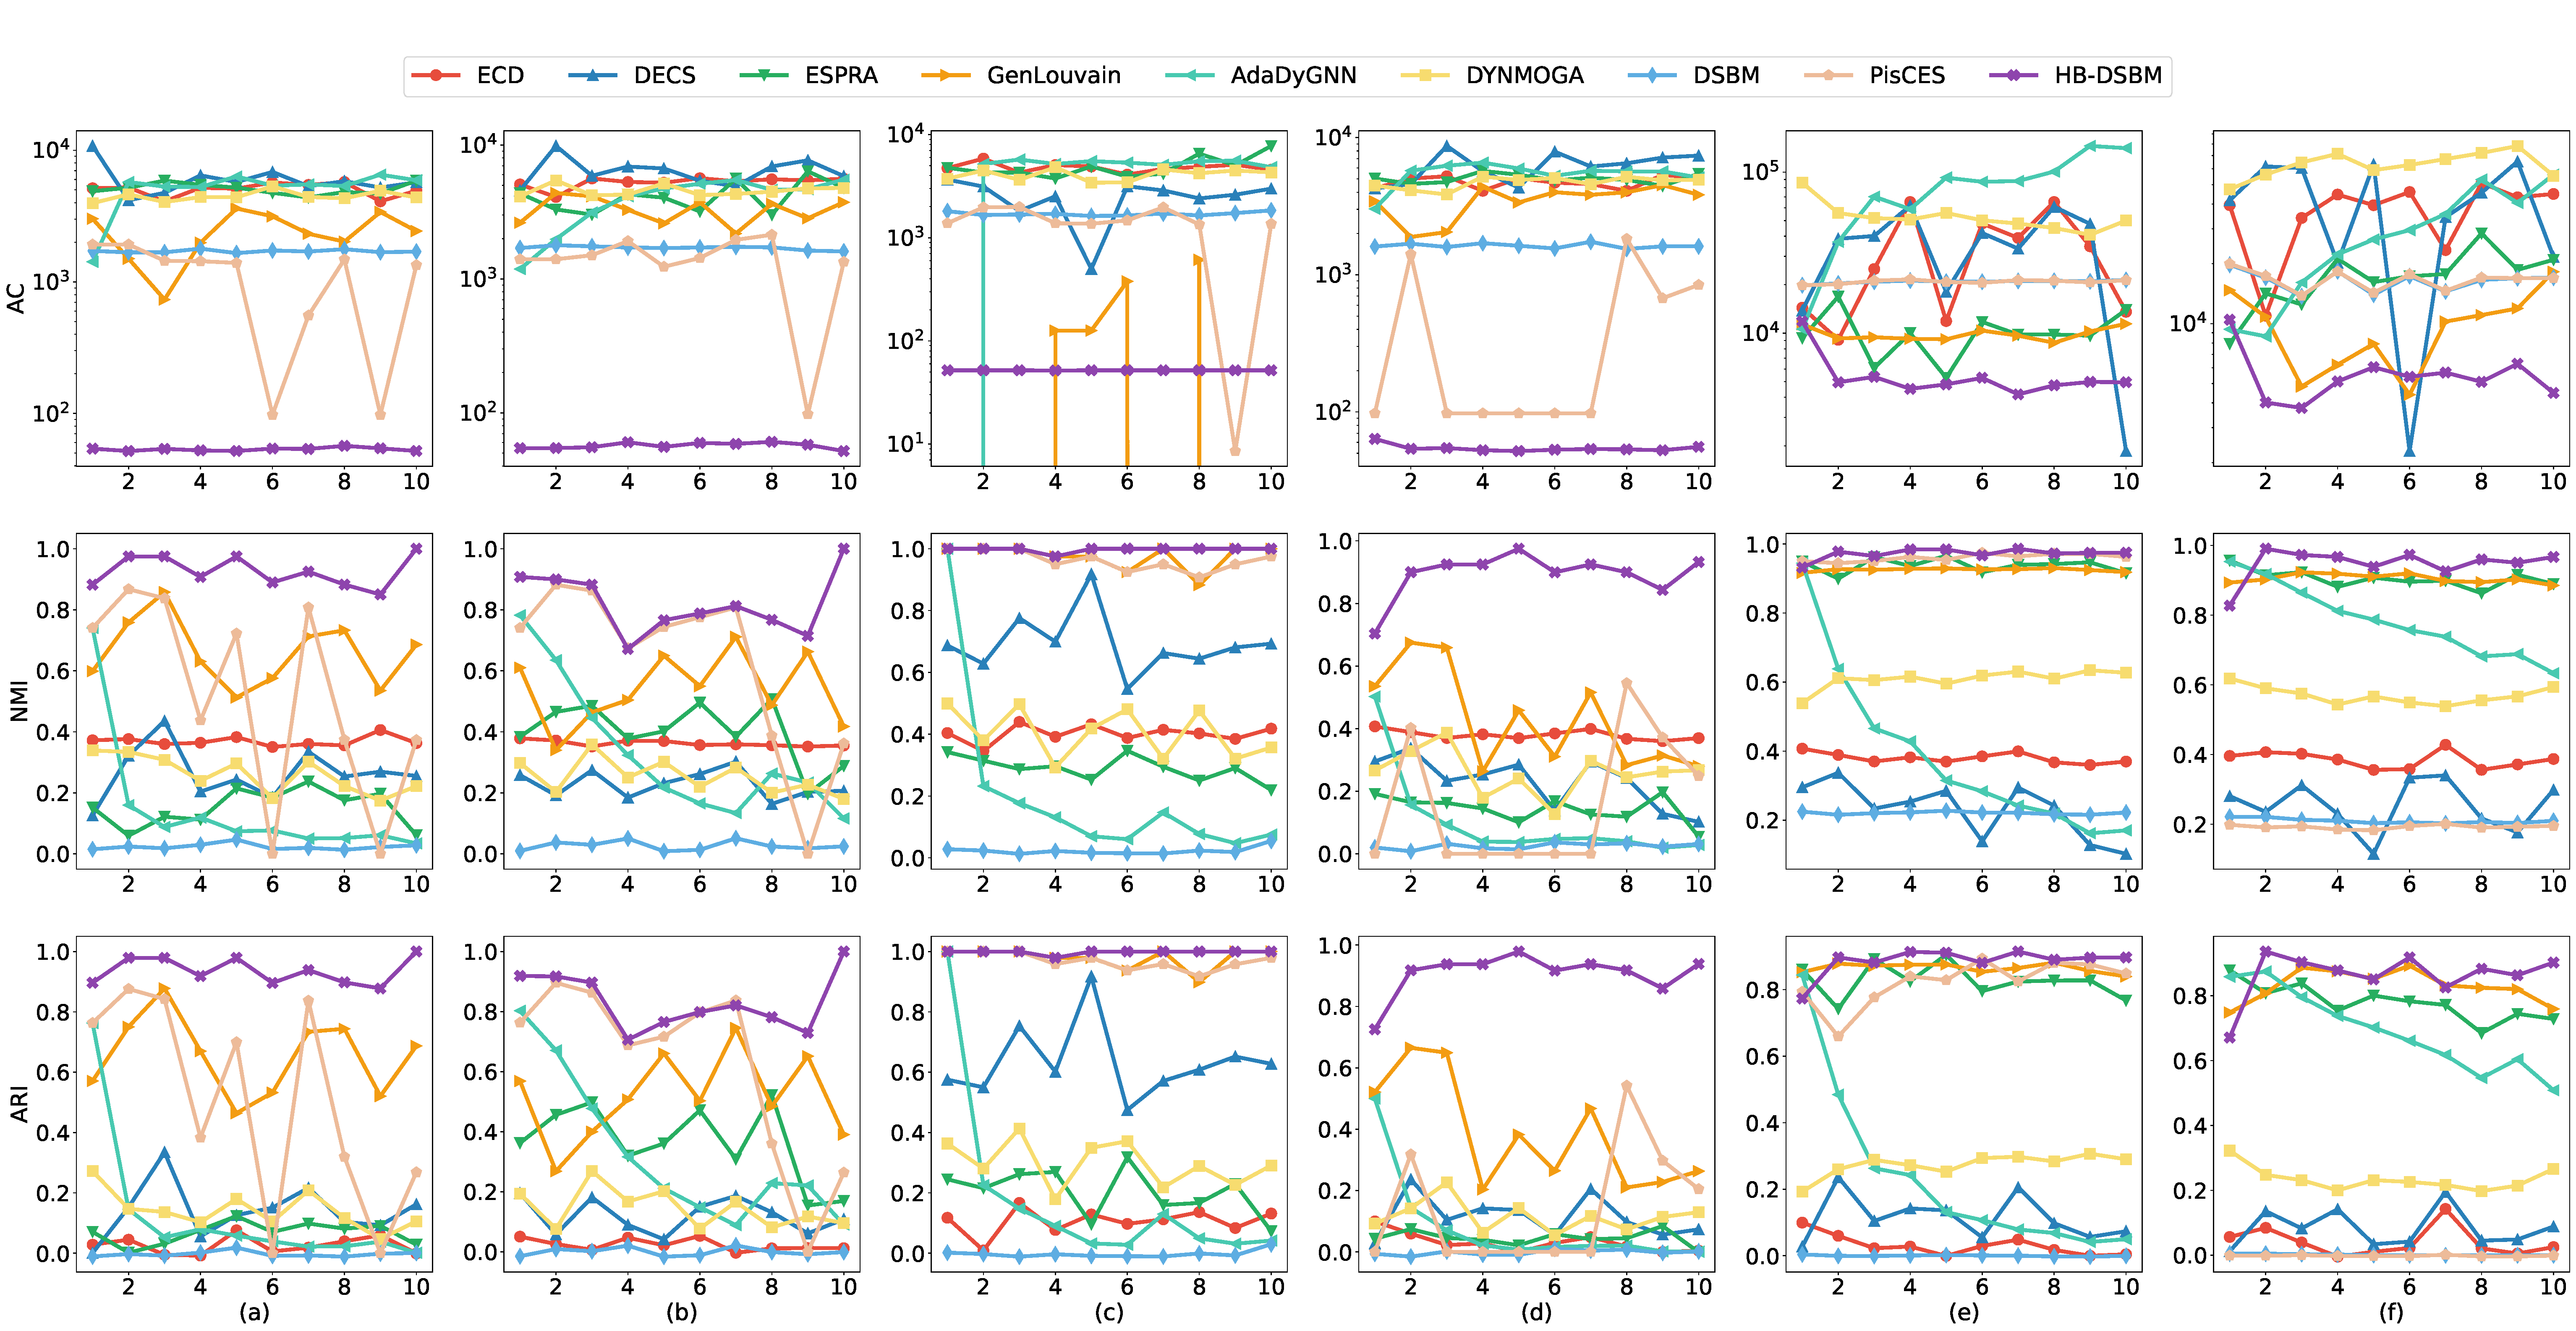
\includegraphics[width=\textwidth]{figures/chap03/dsbm/chap3generateData1223.pdf}
	\caption{生成数据集中的社团检测结果}
	\label{fig.4.2}
\end{figure}



真实世界数据集的实验结果如图~\ref{fig.4.4}。图~\ref{fig.4.4}中前三列为Kit-email数据按照不同时间间隔划分的结果,最后一列为DBLP数据集的社团检测结果。其展示了HB-DSBM对于真实世界数据的社团检测的优异能力,证明了本方法所刻画的节点演化异质性更加符合真实世界网络演化。值得注意的是,在第一个快照中,HB-DSBM的设计与静态随机块模型一致,因此本方法的优势在第一个快照并不明显,而随着时间推移,HB-DSBM对动态网络的建模优势逐渐显现。



\begin{figure}[htbp]
	\centering
	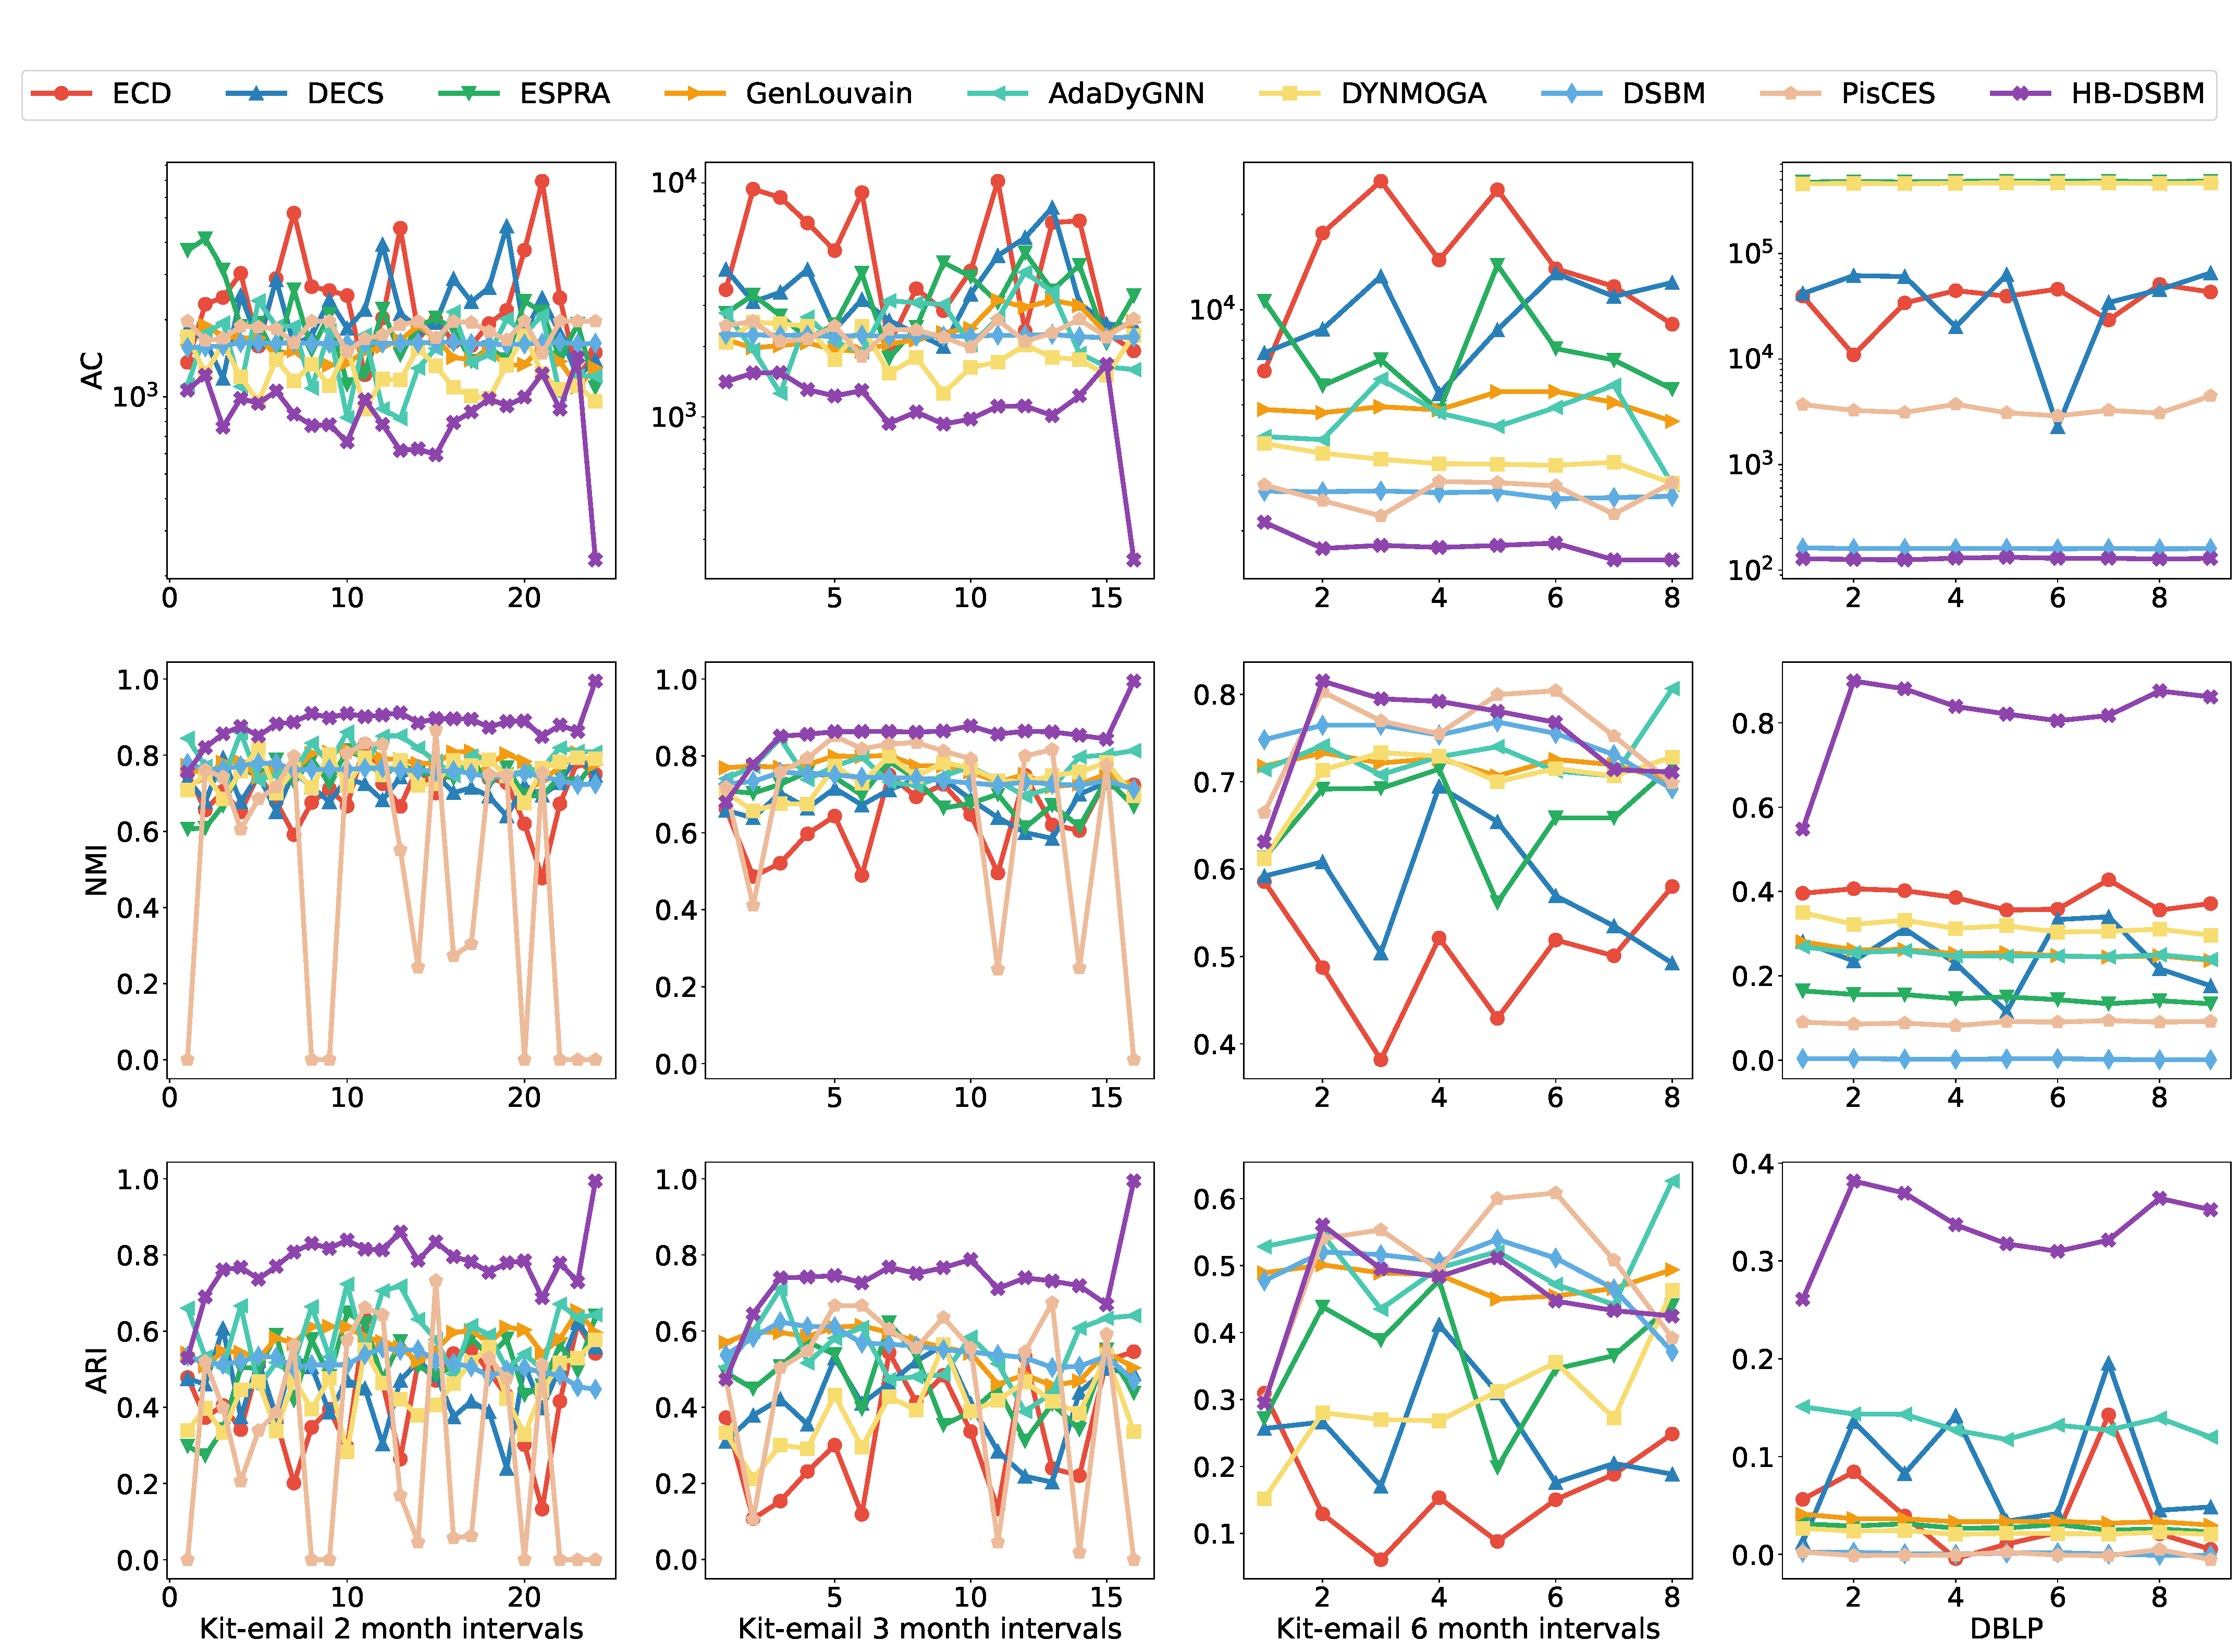
\includegraphics[width=0.9\textwidth]{figures/chap03/dsbm/chap3realData1223.pdf}
	\caption{真实世界数据的社团检测结果}
	\label{fig.4.4}
\end{figure}




\subsection{社团演化分析}


社团演化方面,本节分别针对生成数据1、生成数据2以及DBLP数据进行了社团演化的可视化展示,如图~\ref{fig:SankeyFacetnet}~\ref{fig:SankeyAsonamMS}和图~\ref{fig:SankeyDBLP}所示,其中第一个GroundTruth代表社团真相。需要注意的是,由于ESPRA和AdaDyGNN在生成数据2与DBLP数据中的社团演化效果较差,因此图中进行了省略。由图中可以看出,HB-DSBM能够准确的刻画动态网络的社团演化,且对于复杂的社团演化行为均具有较好的刻画能力。而DSBM由于缺少节点演化异质性假设,因此其难以建模复杂的社团演化行为,而其余方法如PisCES、DYNMOGA等由于模型设计的问题,呈现出了混乱的社团演化行为,难以正确刻画社团的演化,因此无法支撑对动态网络社团演化的分析。



\begin{figure}
	
	\centering
	\subfigure[GroundTruth]{
		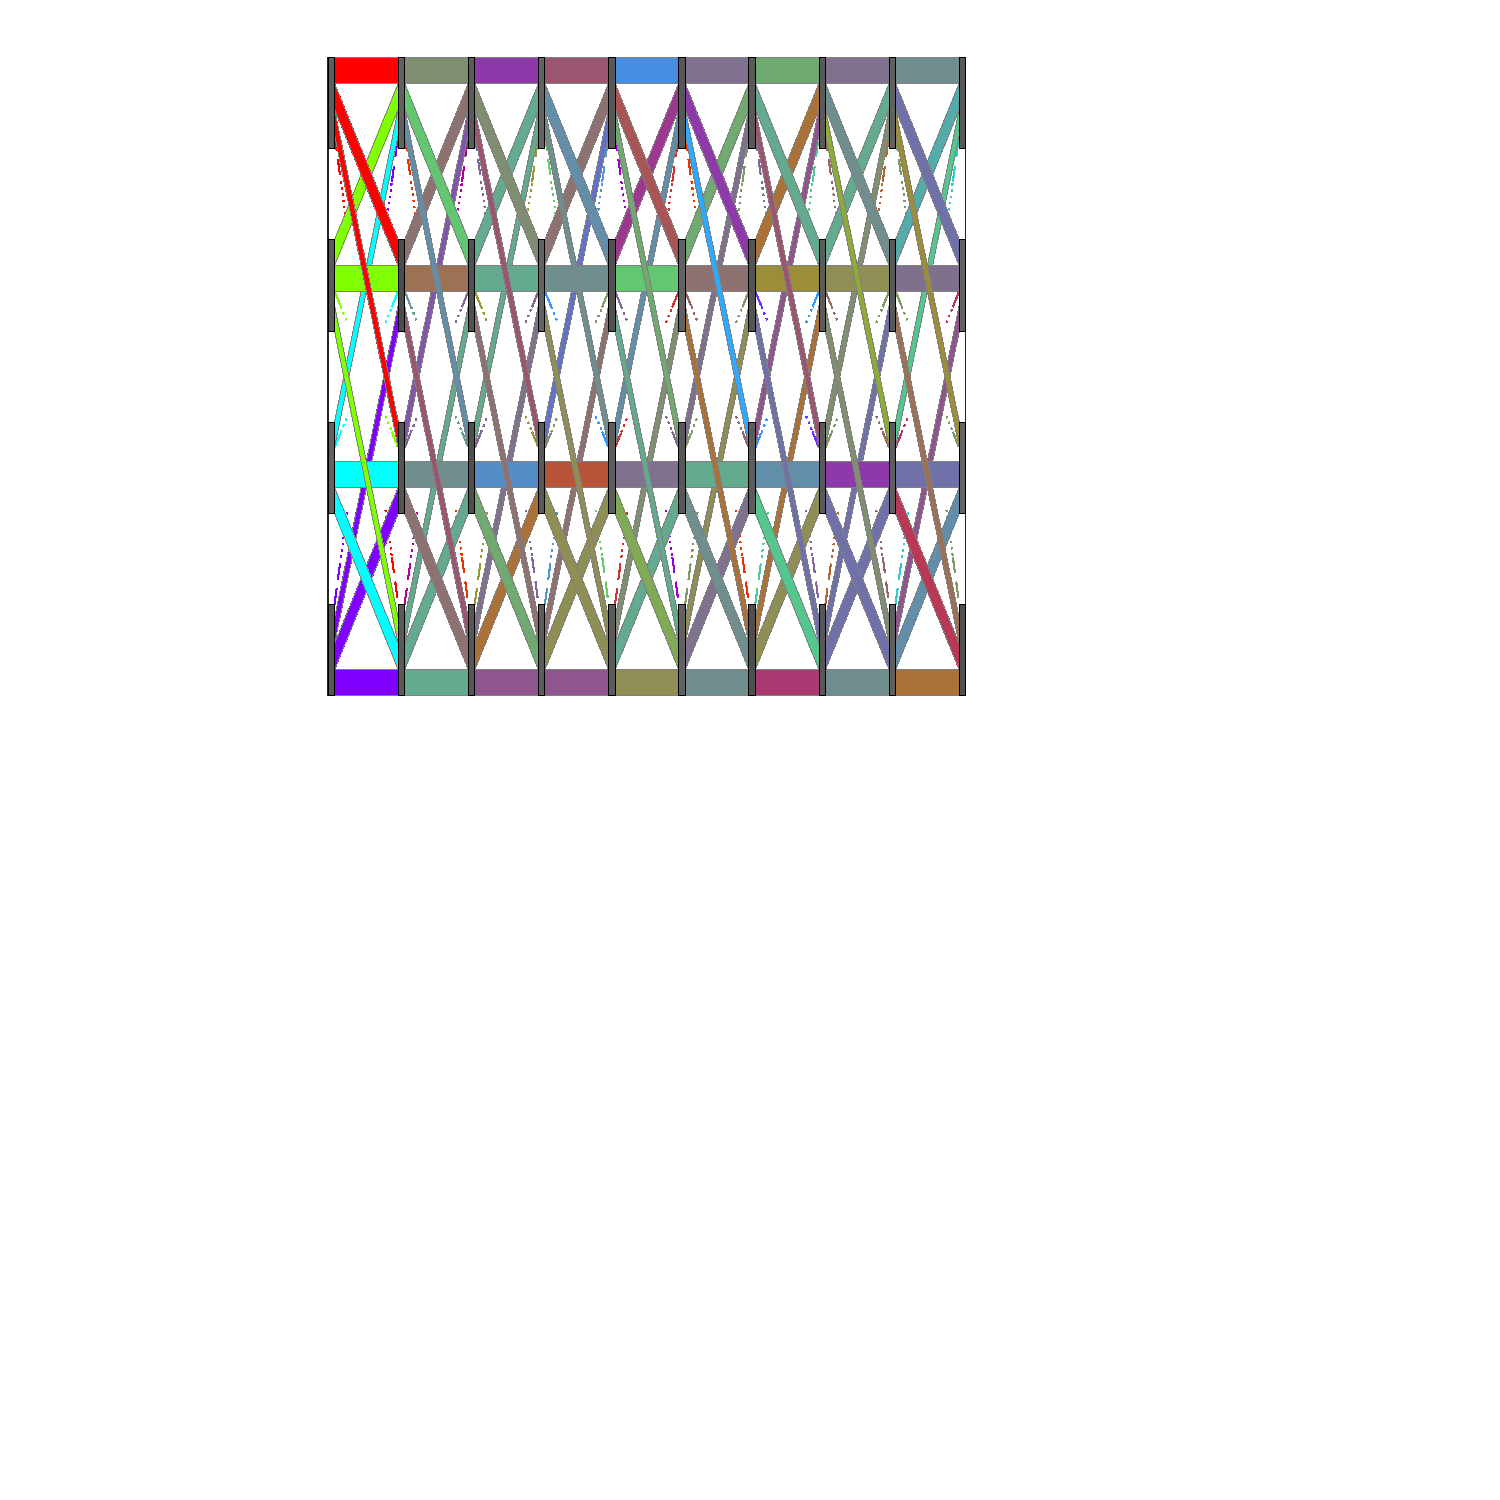
\includegraphics[width=.24\textwidth,height=.125\textwidth]{figures/chap03/dsbm/facetNetEvolution/groundTruth.pdf}
	}
	\subfigure[DSBM]{
		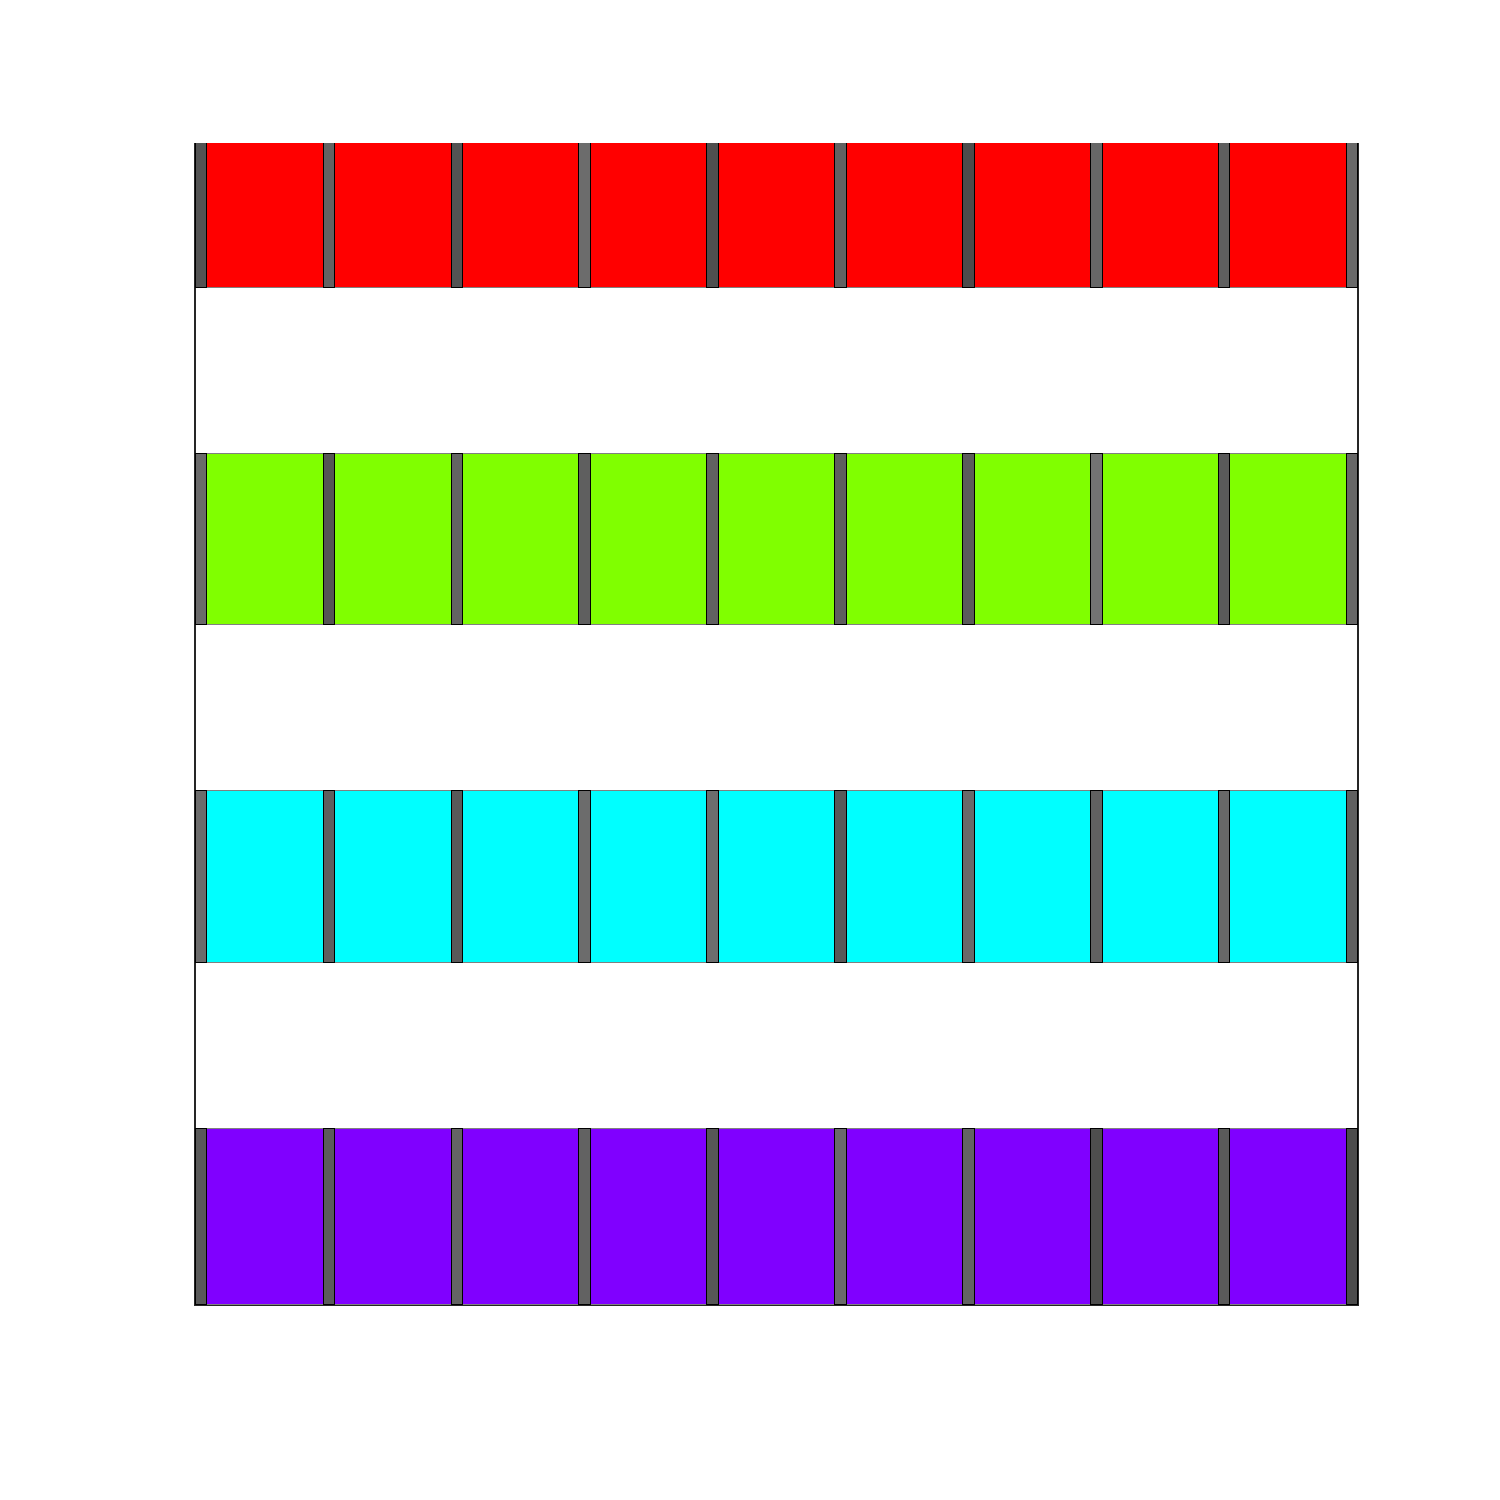
\includegraphics[width=.24\textwidth,height=.125\textwidth]{figures/chap03/dsbm/facetNetEvolution/DSBM.pdf}
	}
	\subfigure[HB-DSBM]{
		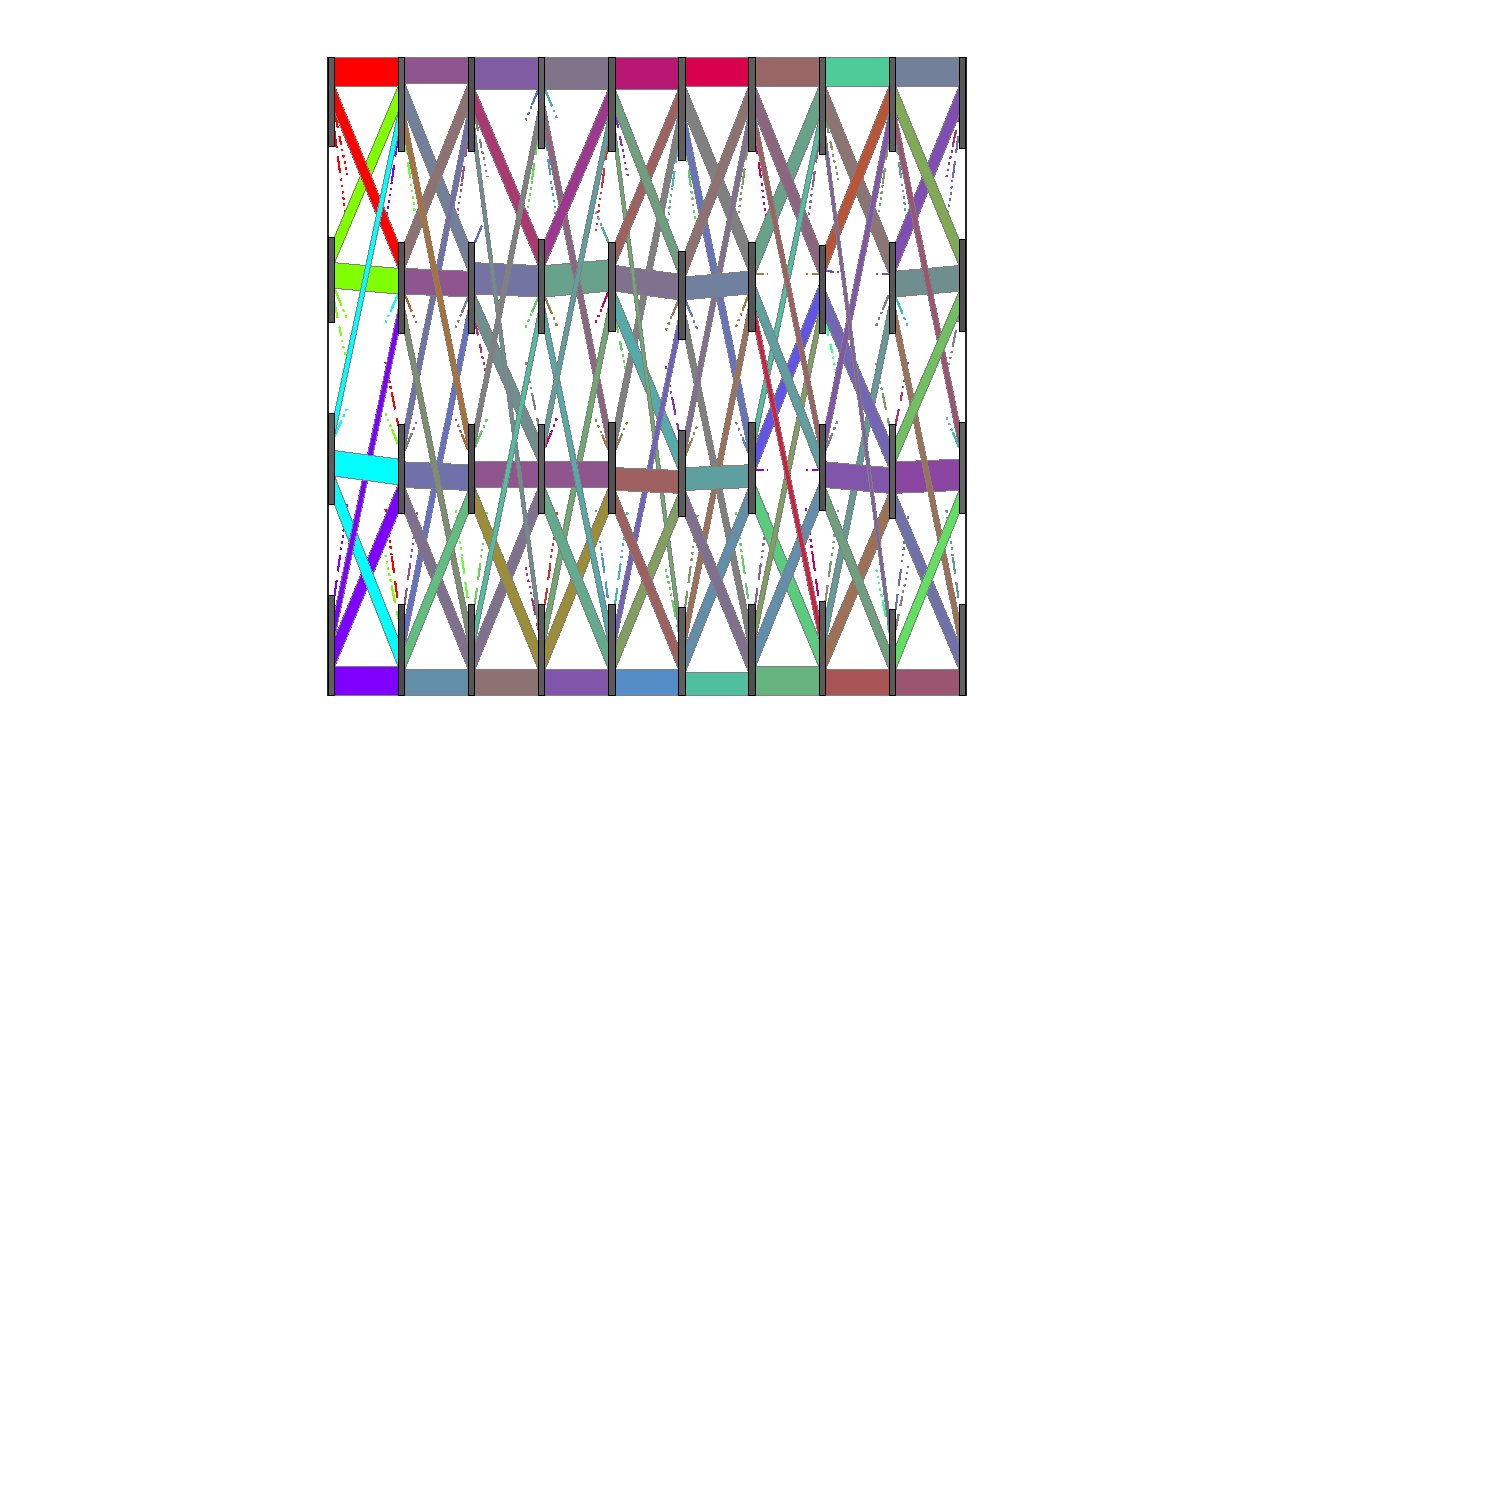
\includegraphics[width=.24\textwidth,height=.125\textwidth]{figures/chap03/dsbm/facetNetEvolution/HBDSBM.pdf}
	}
	\subfigure[GenLouvain]{
		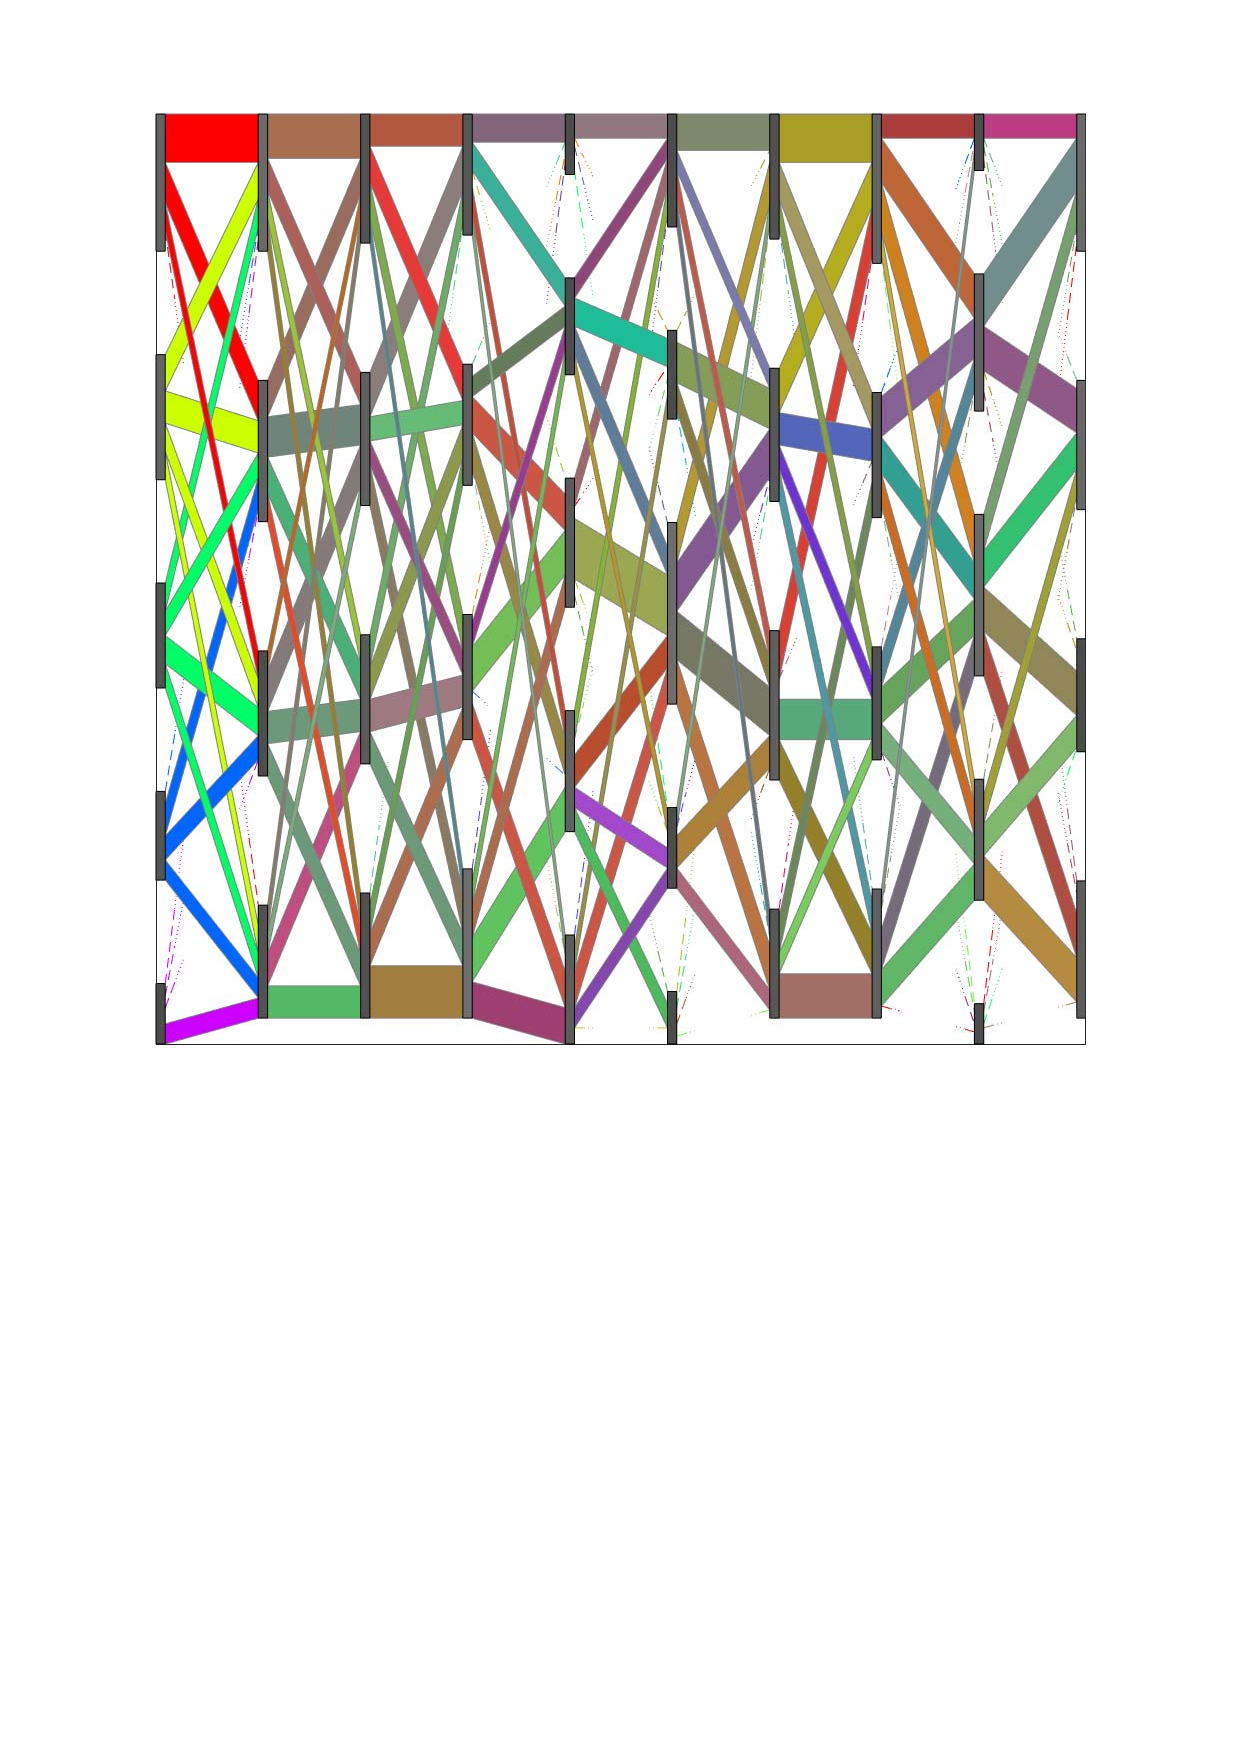
\includegraphics[width=.24\textwidth,height=.125\textwidth]{figures/chap03/dsbm/facetNetEvolution/gen.pdf}
	}
	\subfigure[PisCES]{
		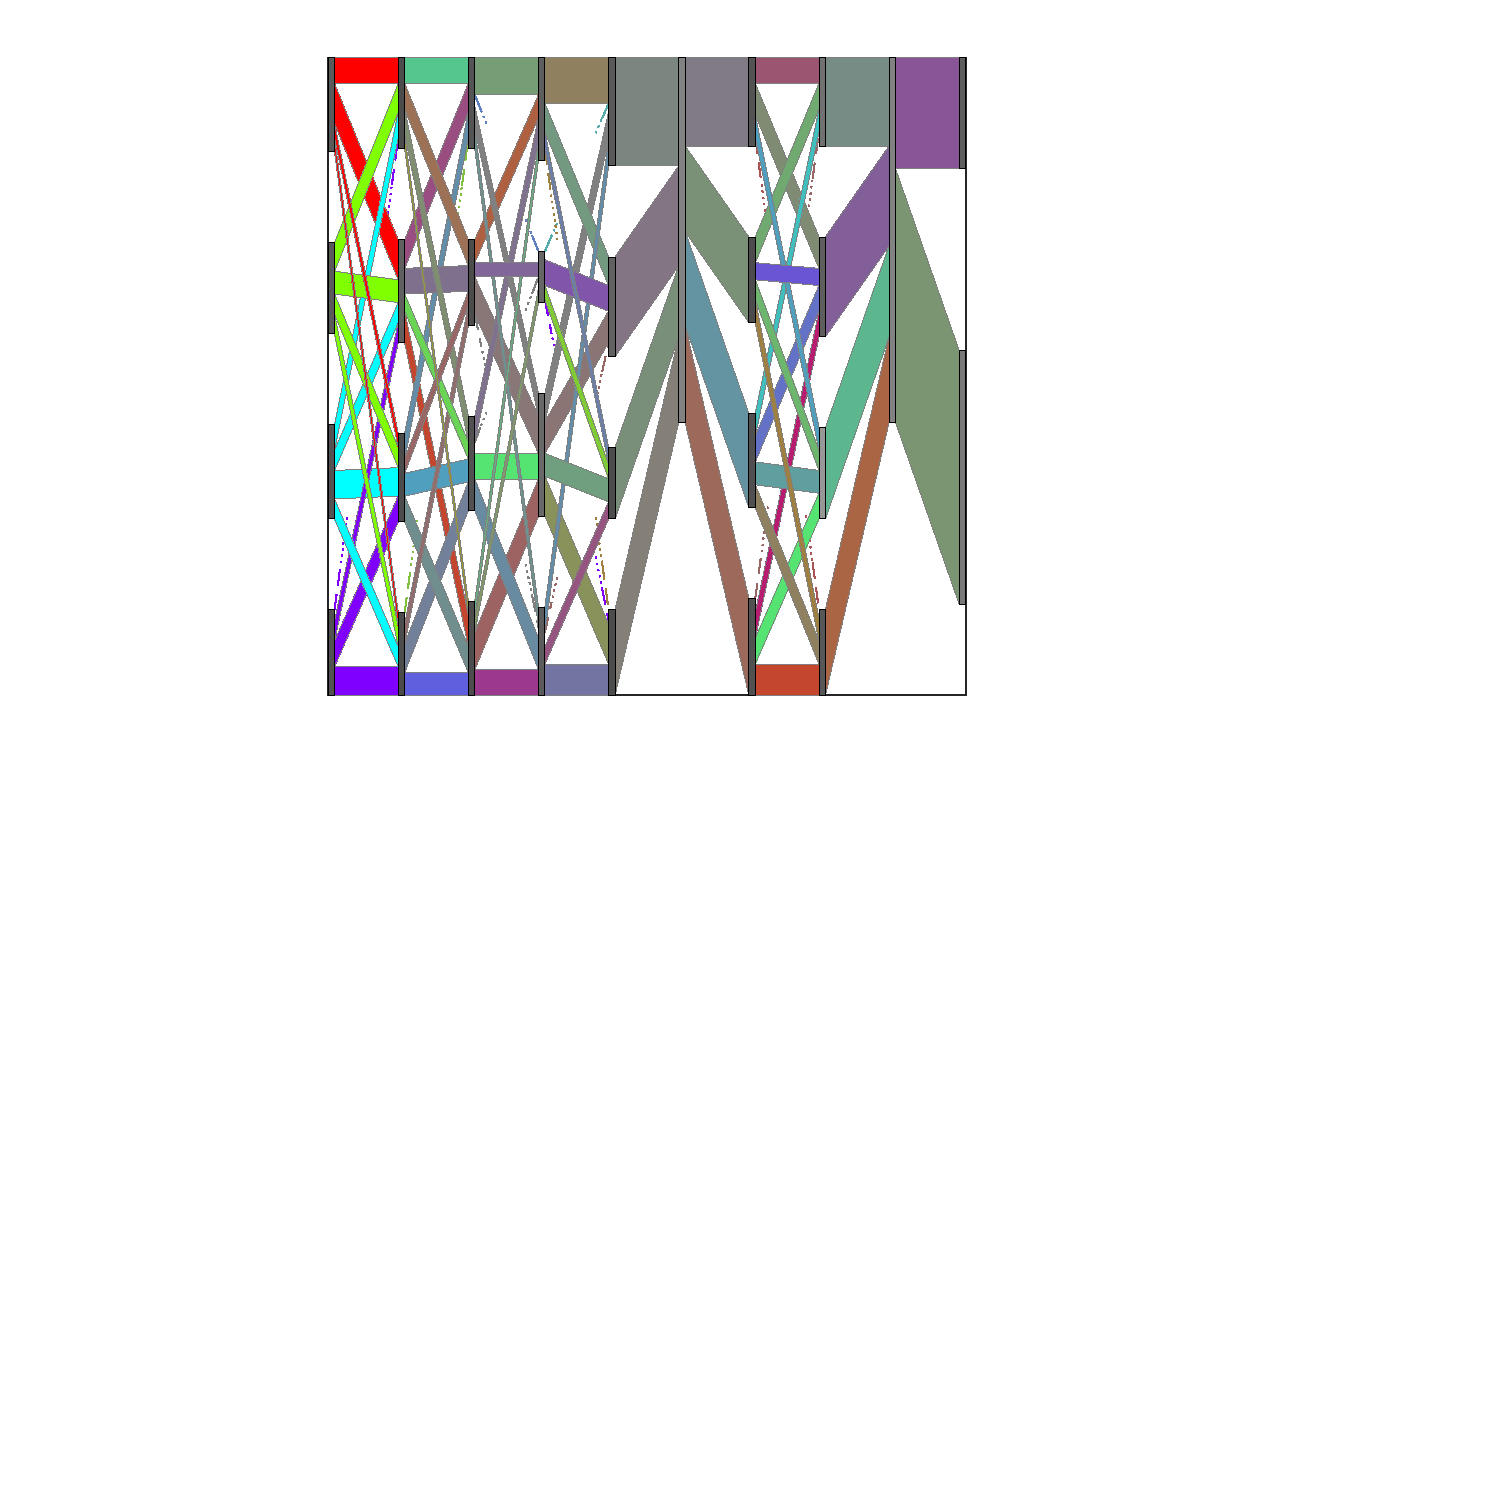
\includegraphics[width=.24\textwidth,height=.125\textwidth]{figures/chap03/dsbm/facetNetEvolution/PisCES.pdf}
	}
	\subfigure[DYNMOGA]{
		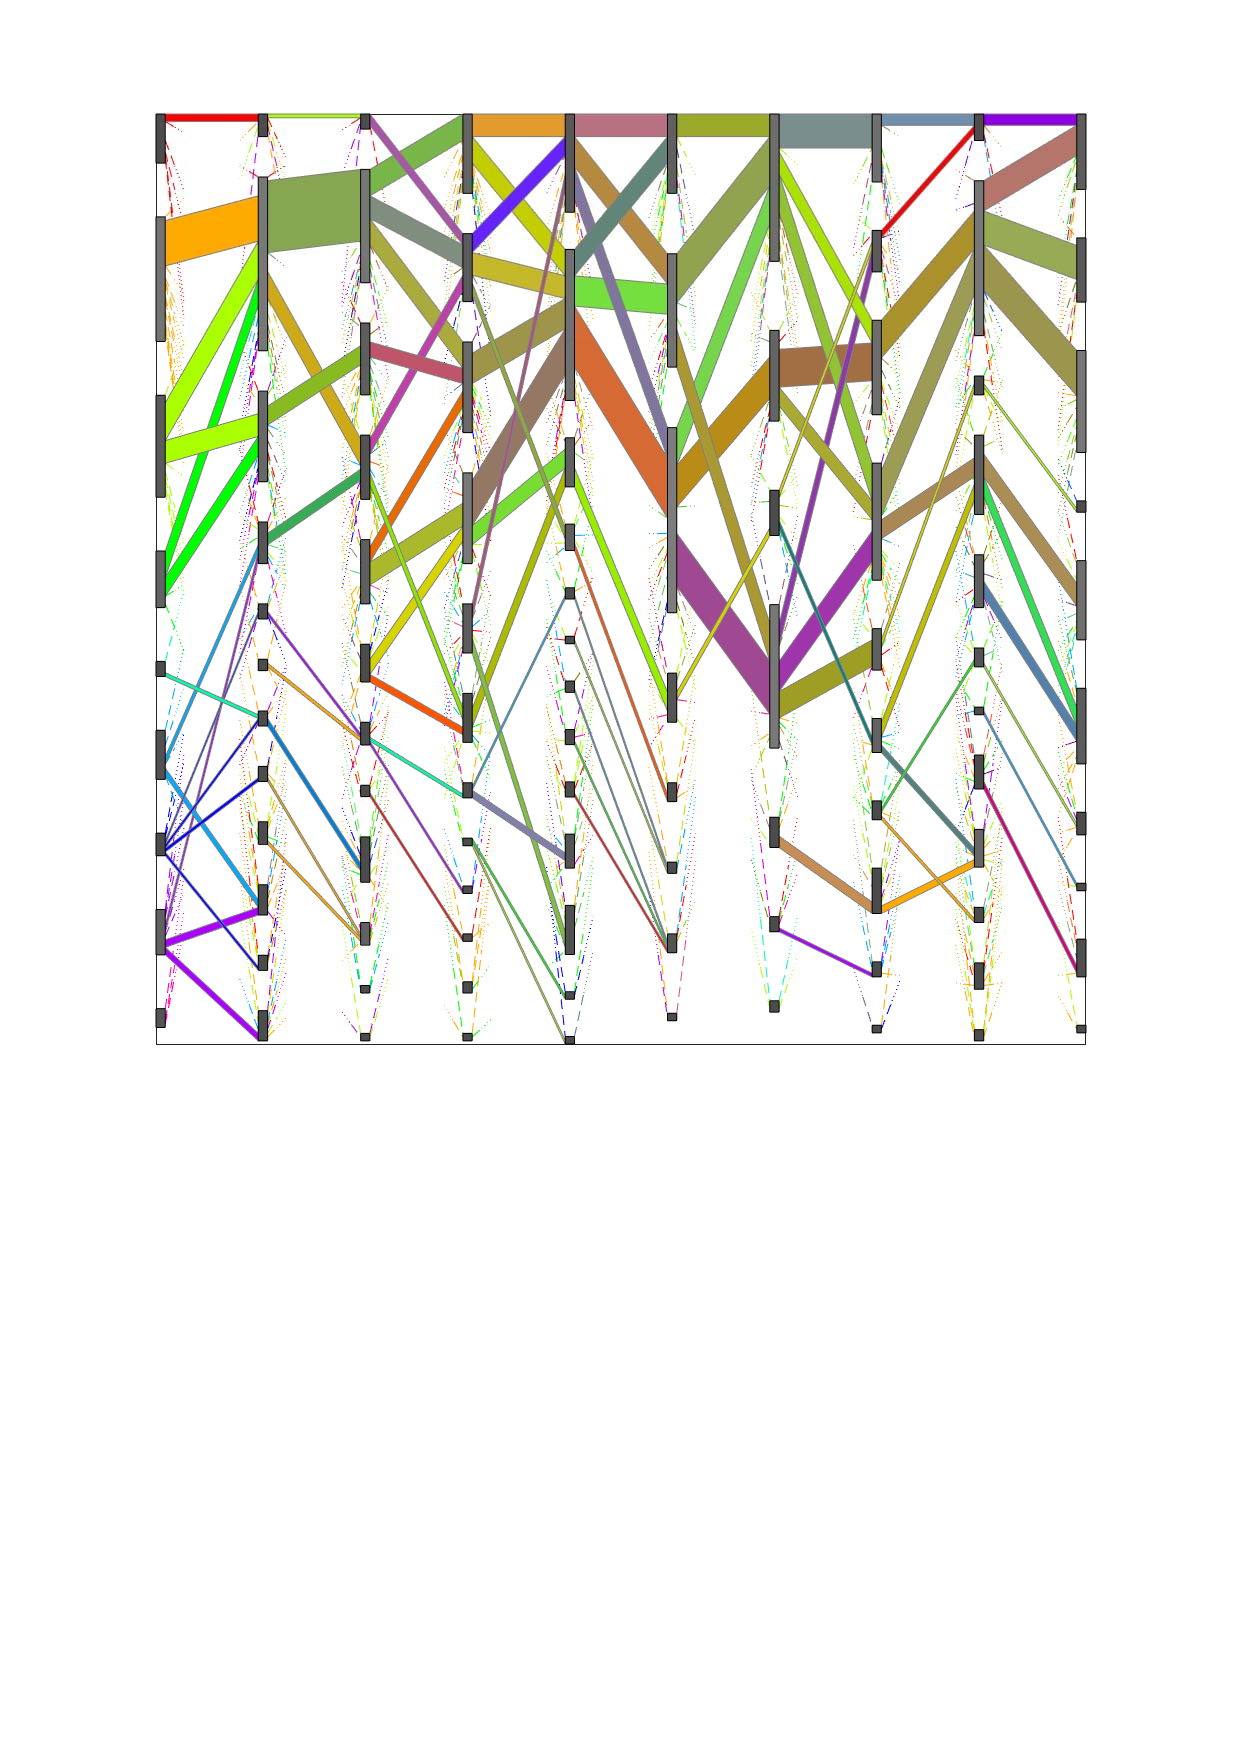
\includegraphics[width=.24\textwidth,height=.125\textwidth]{figures/chap03/dsbm/facetNetEvolution/dynmoga.pdf}
	}
	\subfigure[DECS]{
		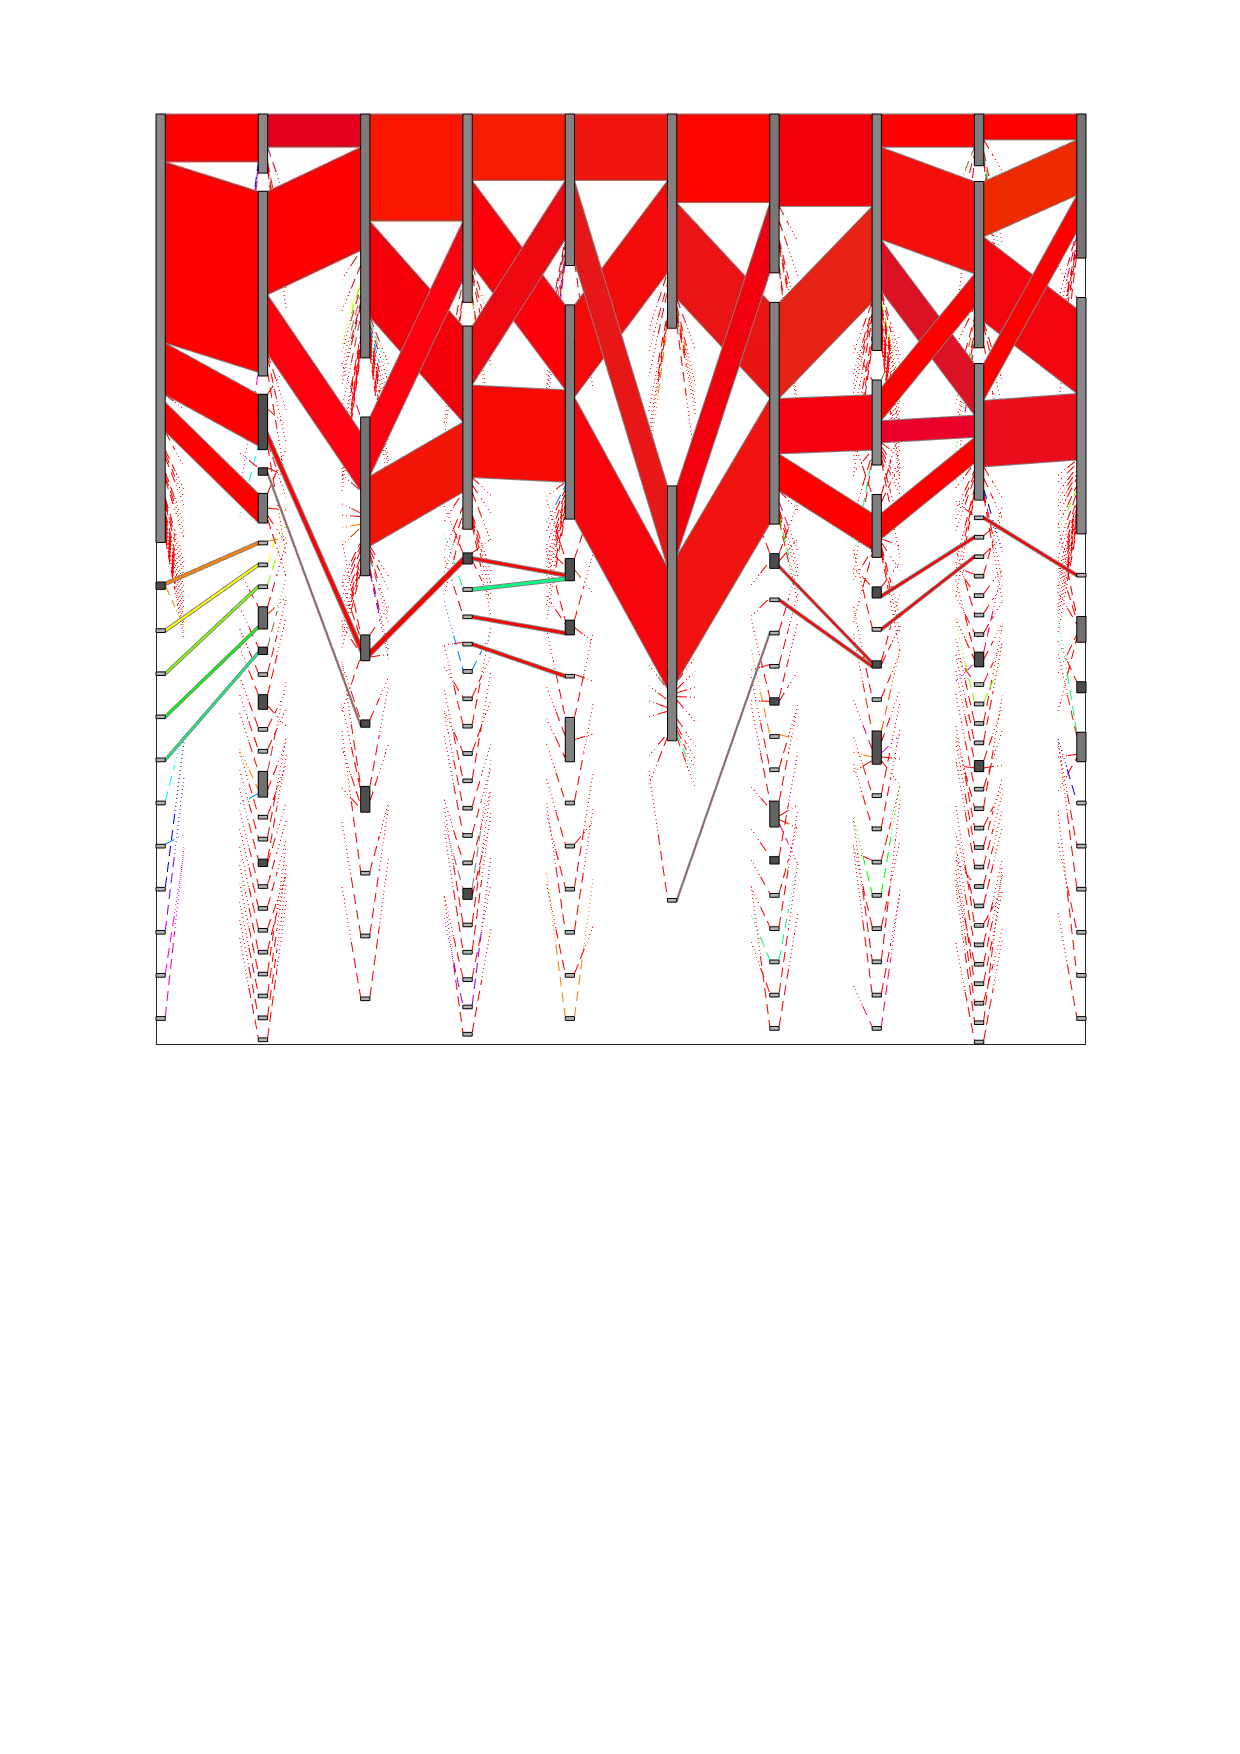
\includegraphics[width=.24\textwidth,height=.125\textwidth]{figures/chap03/dsbm/facetNetEvolution/DECS.pdf}
	}
	\subfigure[ESPRA]{
		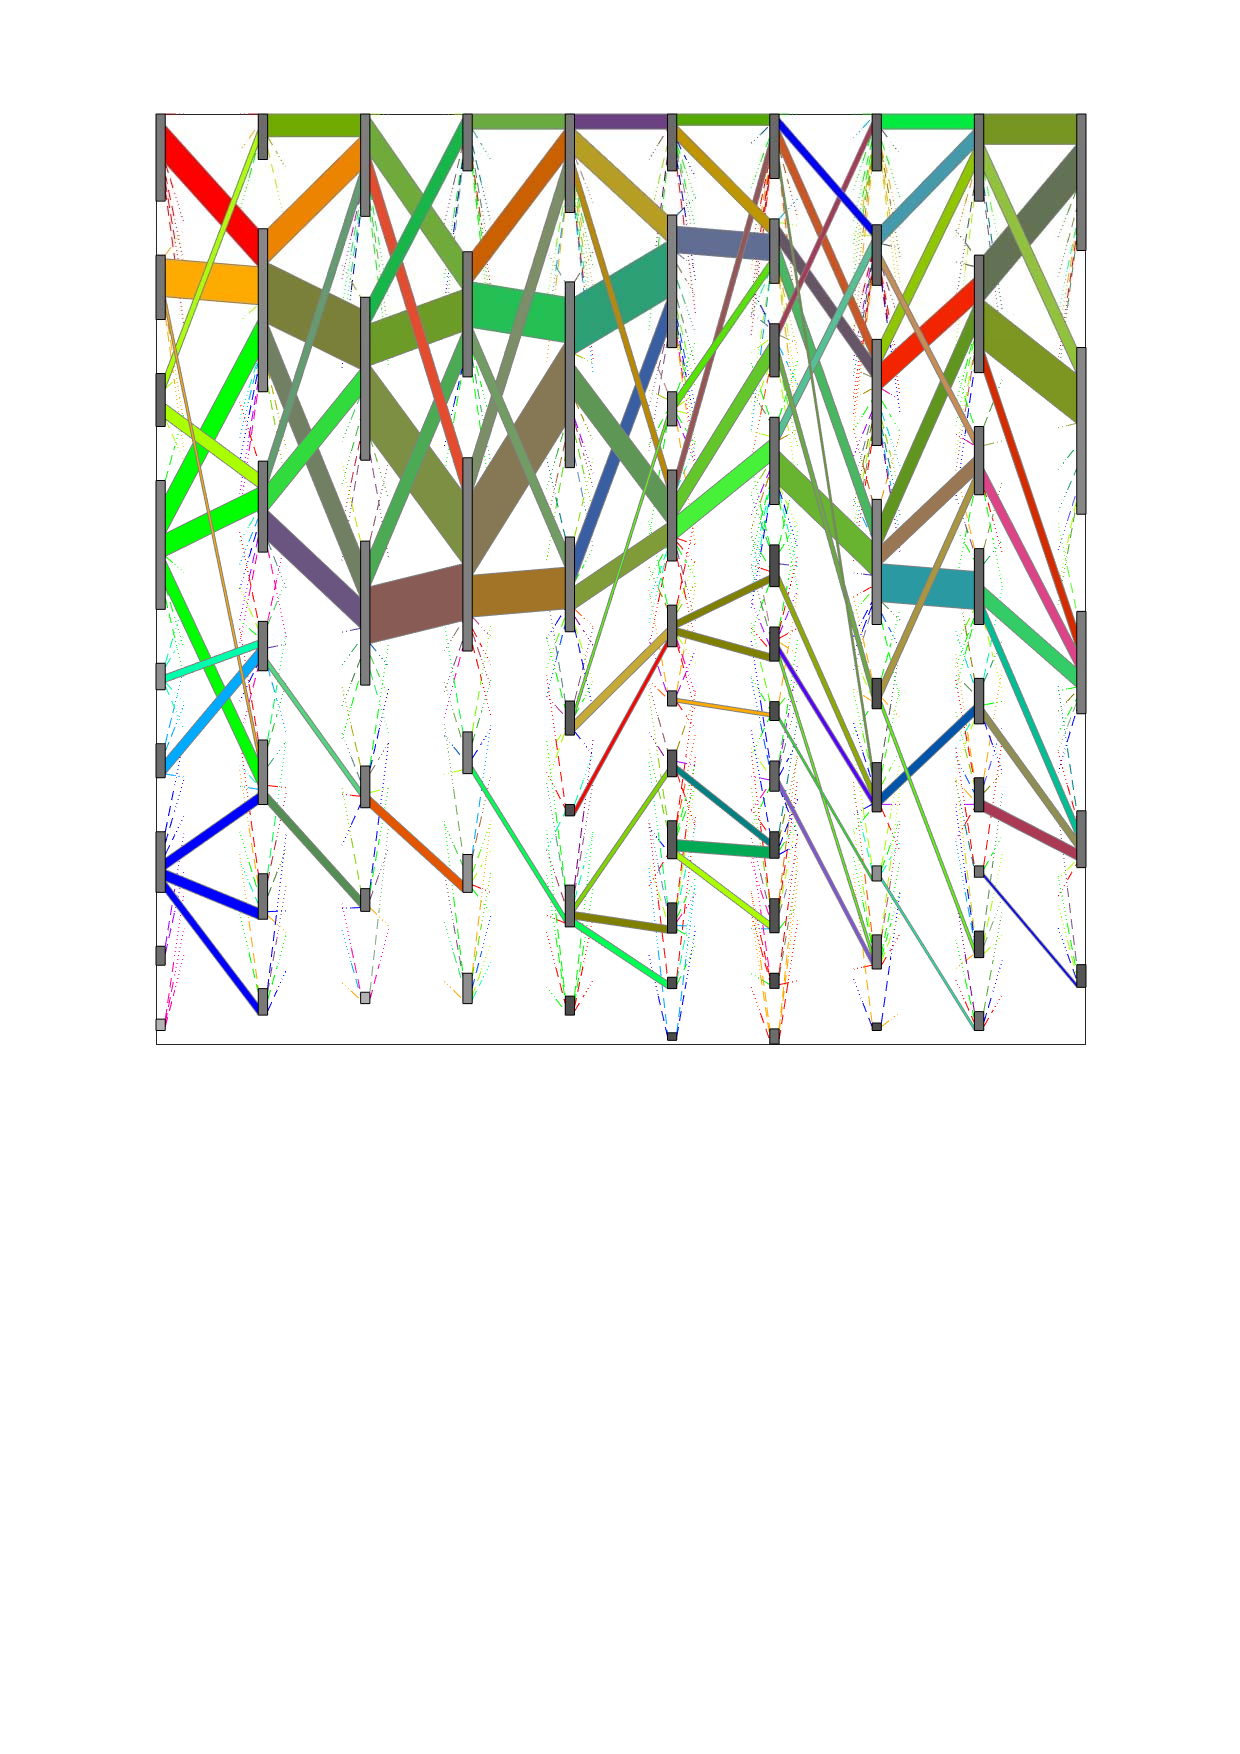
\includegraphics[width=.24\textwidth,height=.125\textwidth]{figures/chap03/dsbm/facetNetEvolution/espra.pdf}
	}
	\subfigure[AdaDyGNN]{
		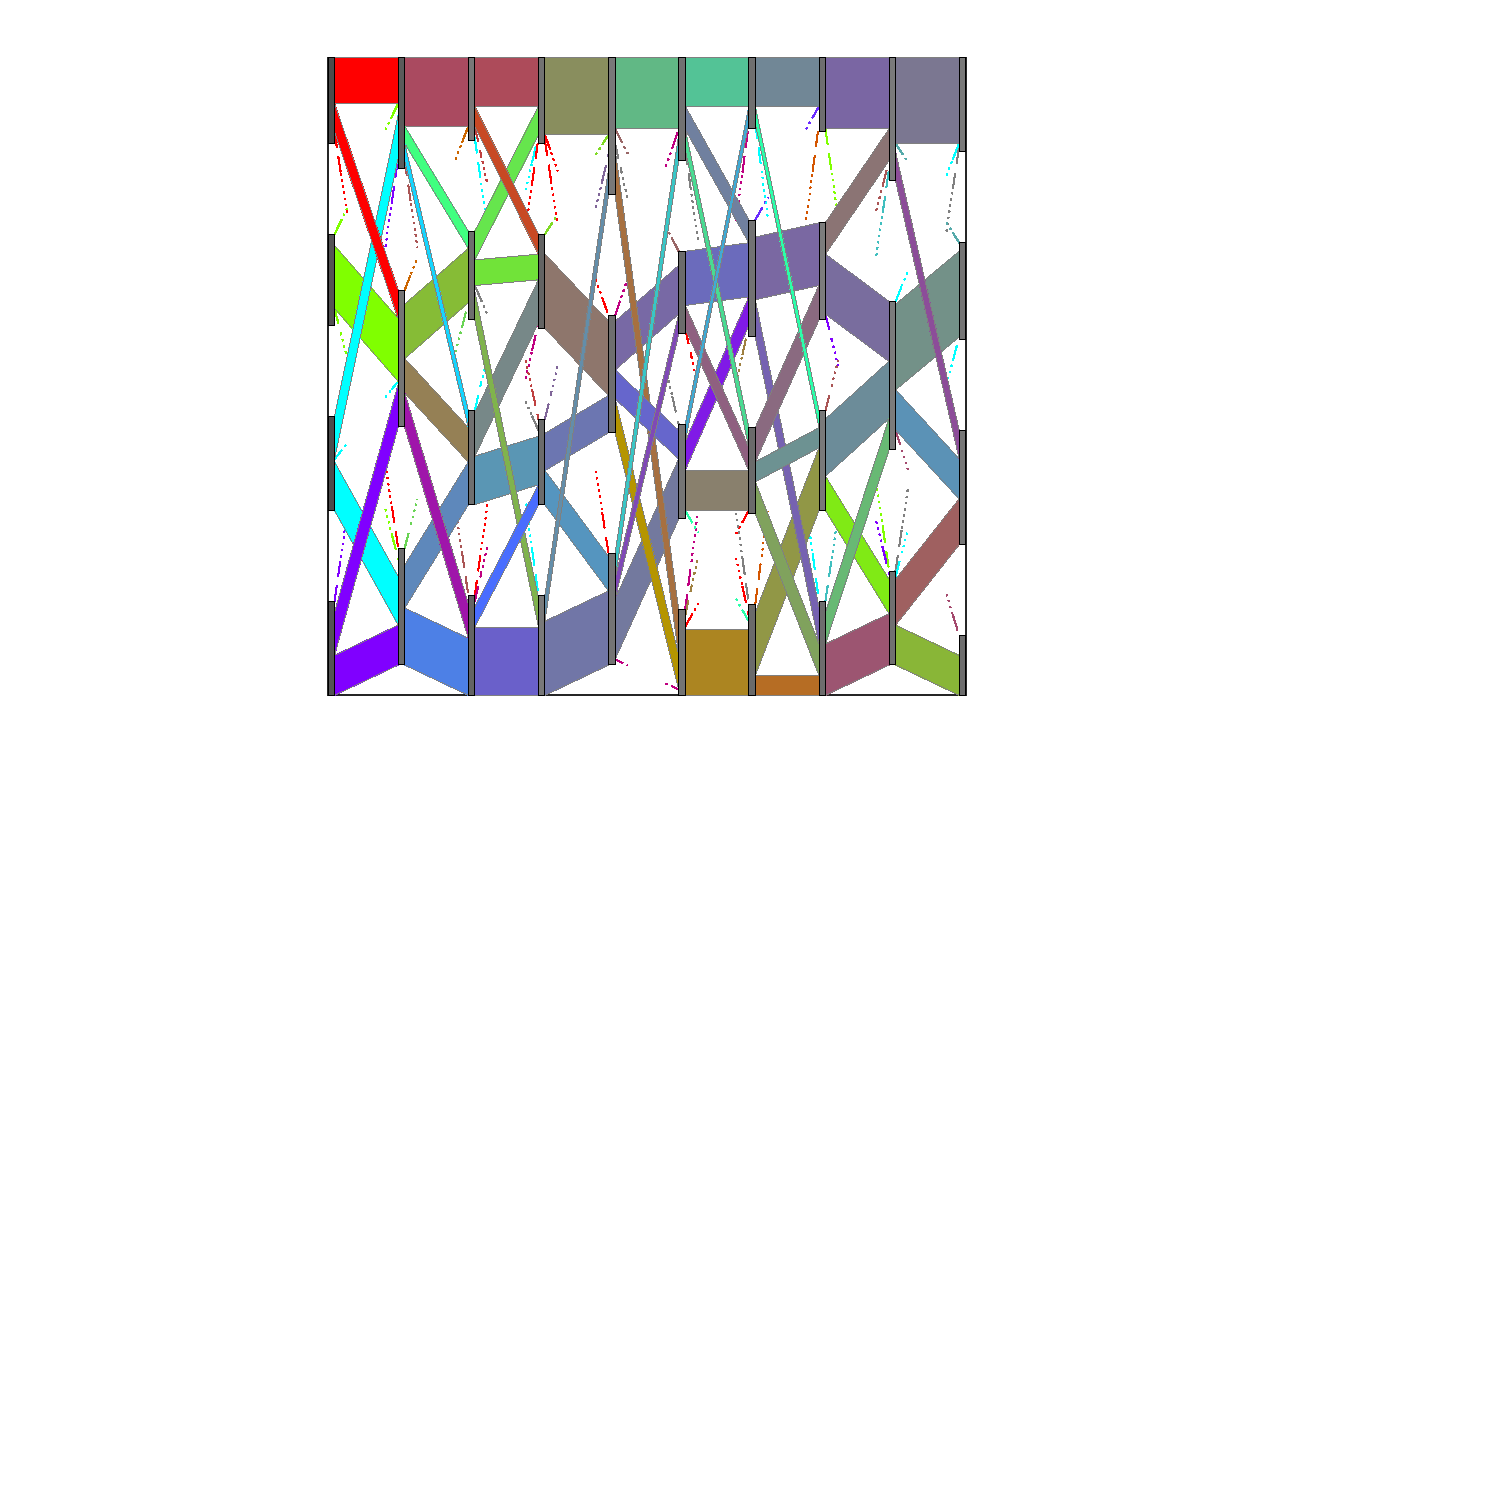
\includegraphics[width=.24\textwidth,height=.125\textwidth]{figures/chap03/dsbm/facetNetEvolution/affect.pdf}
	}
	\caption{生成数据1中参数为$\sigma = 5$, $nC = 9$ and $aD = 20$的社团演化桑基图}
	\label{fig:SankeyFacetnet}
	  \vspace{-1.5cm}
\end{figure}



 \begin{figure}
	\centering
	\subfigure[GroundTruth]{
		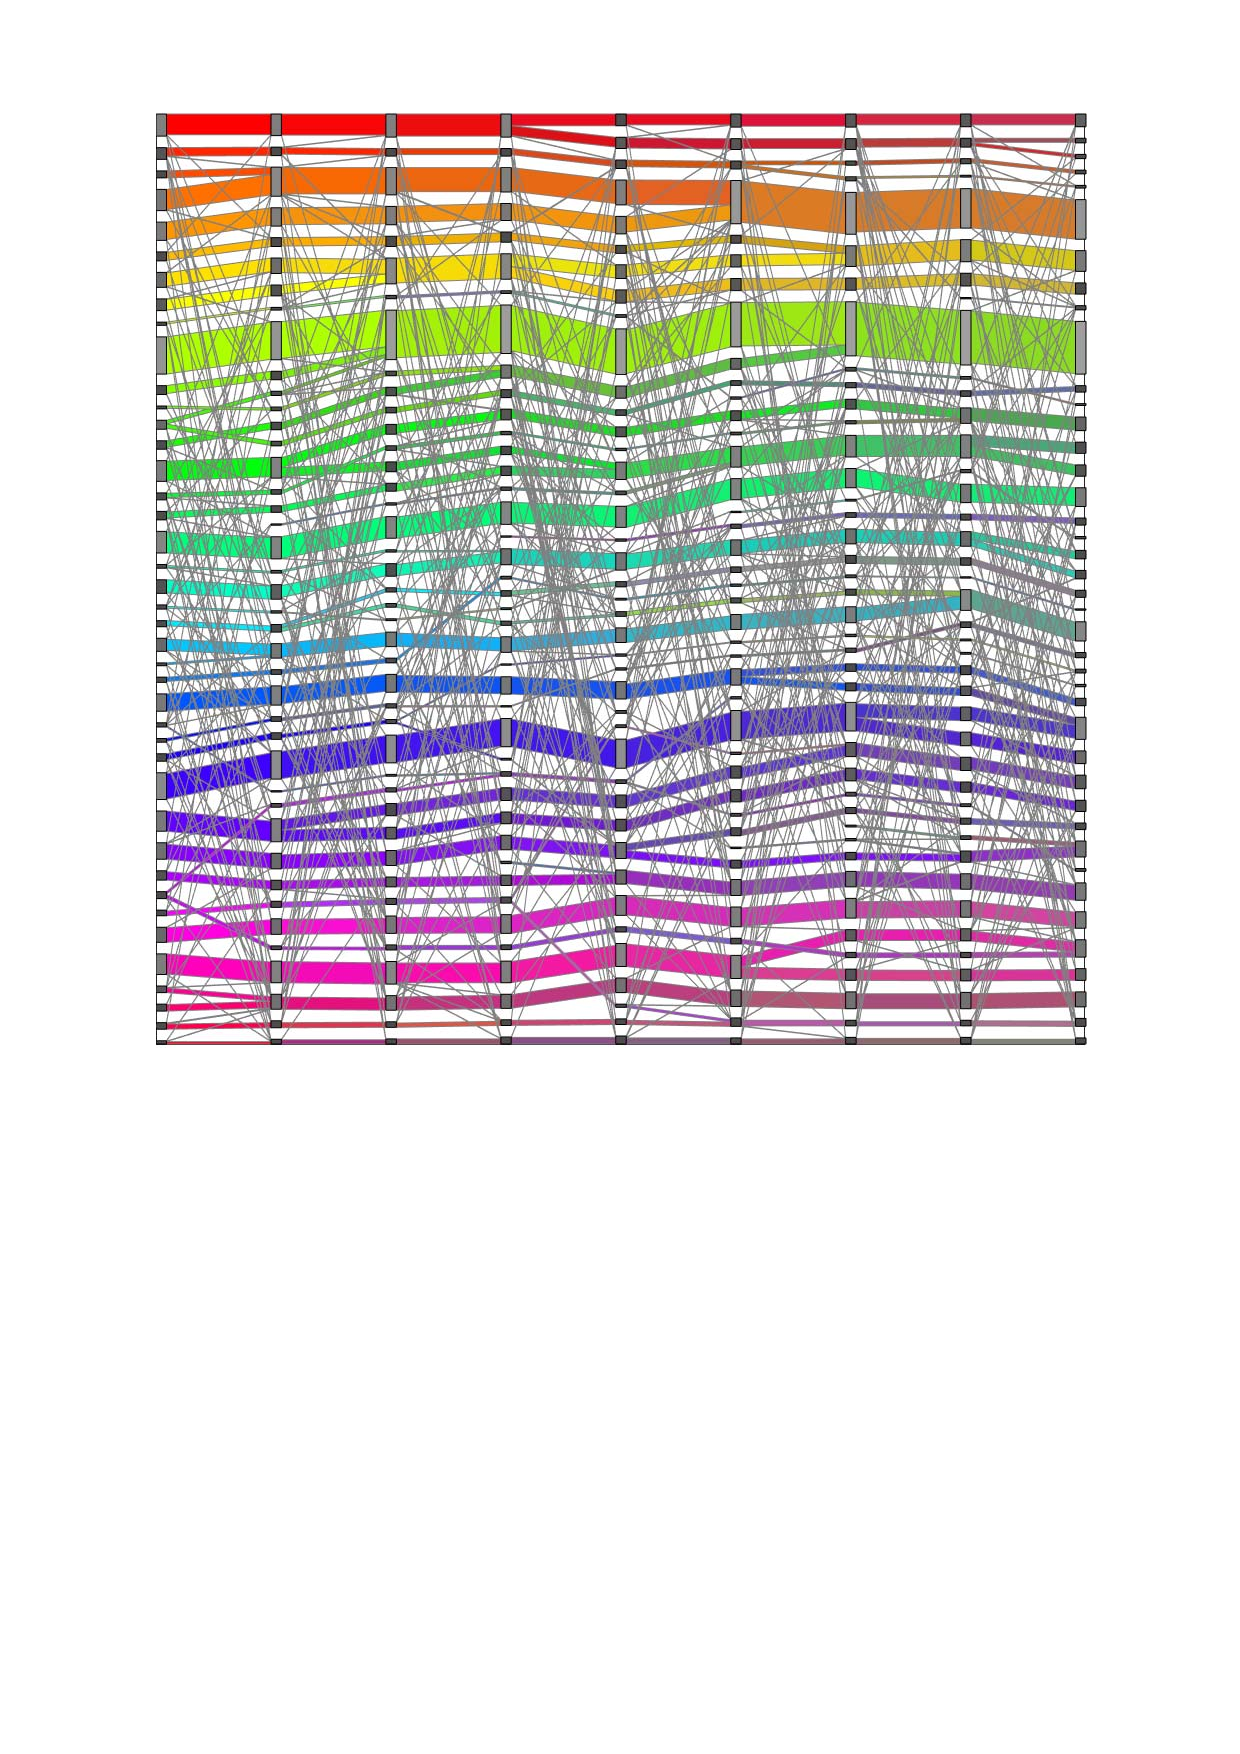
\includegraphics[width=.24\textwidth,height=.15\textwidth]{figures/chap03/dsbm/ASONEMmsEvolution/1GroundTruth.pdf}
	}
	\subfigure[DSBM]{
		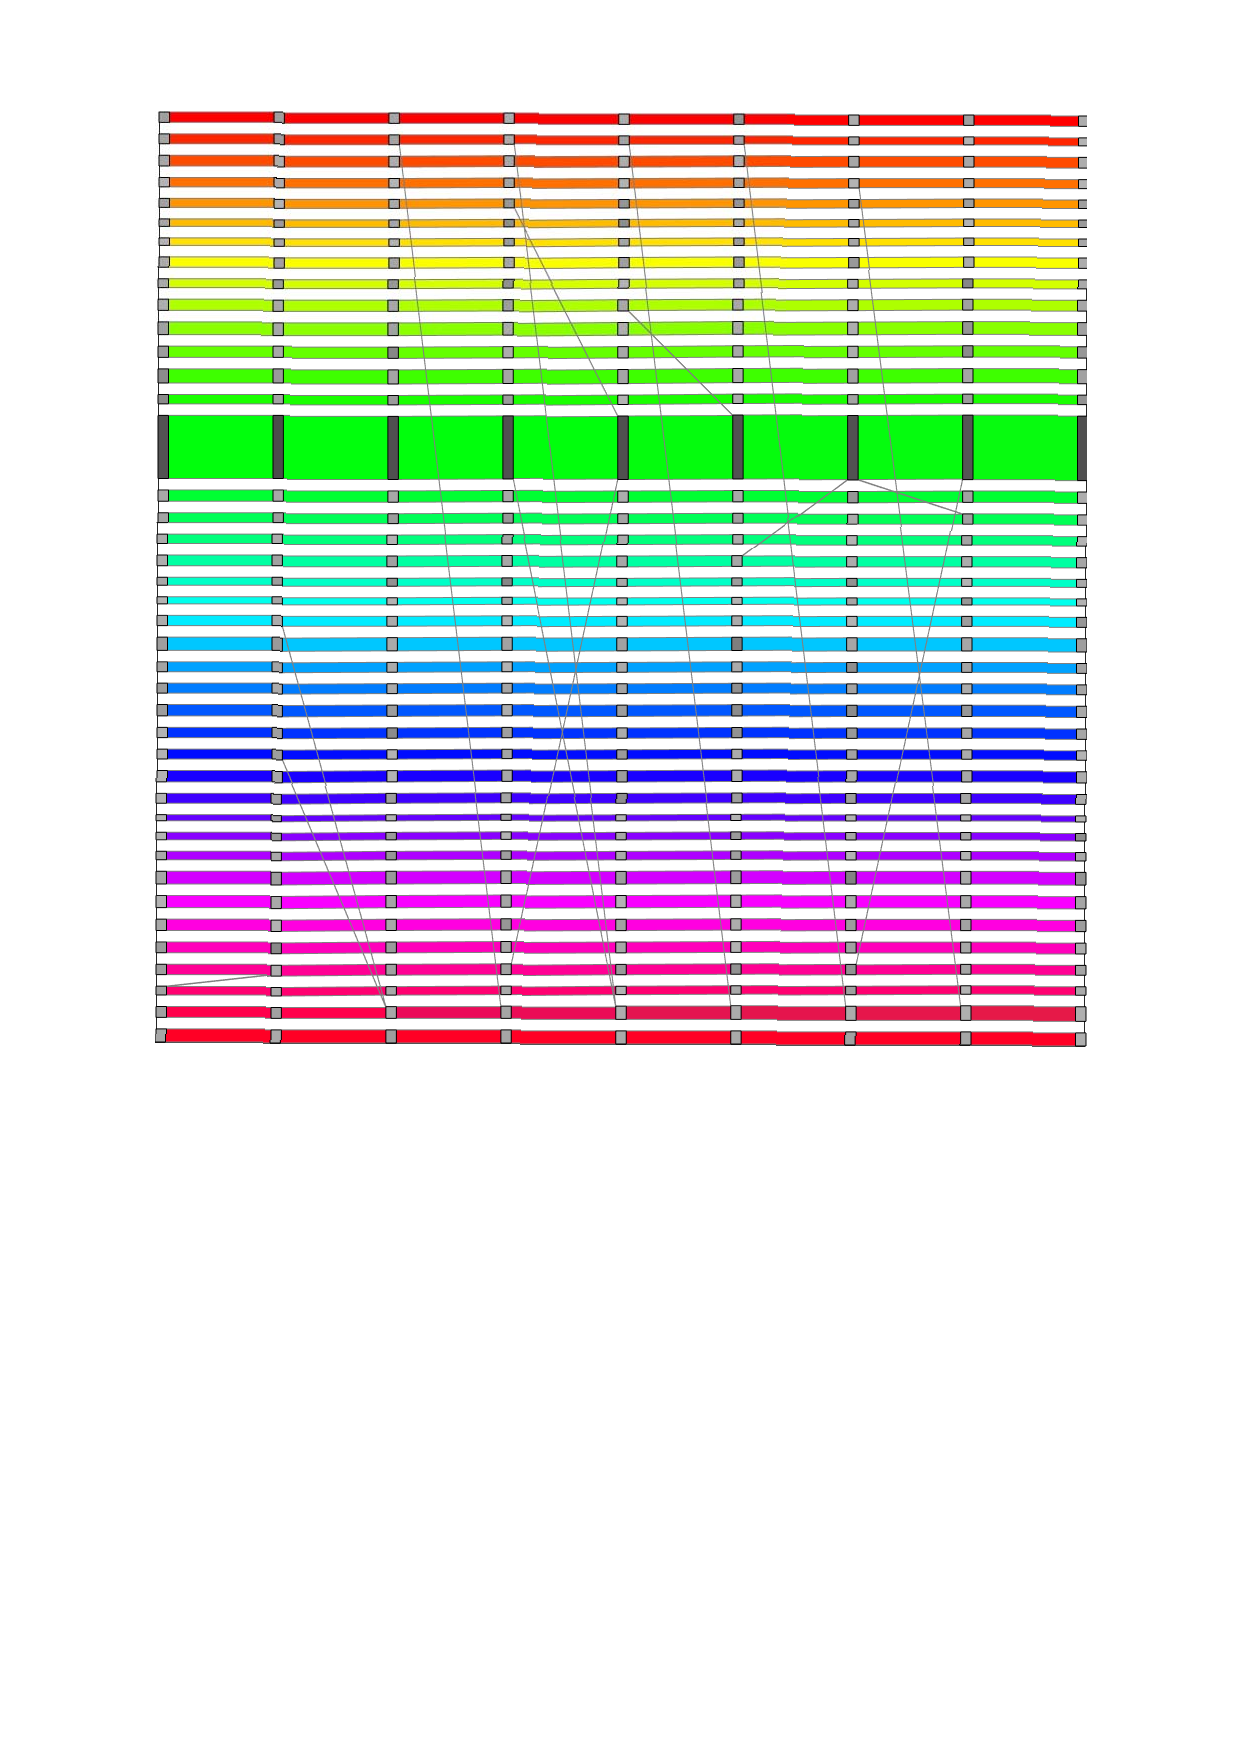
\includegraphics[width=.24\textwidth,height=.15\textwidth]{figures/chap03/dsbm/ASONEMmsEvolution/1DSBM.pdf}
	}
	\subfigure[HB-DSBM]{
		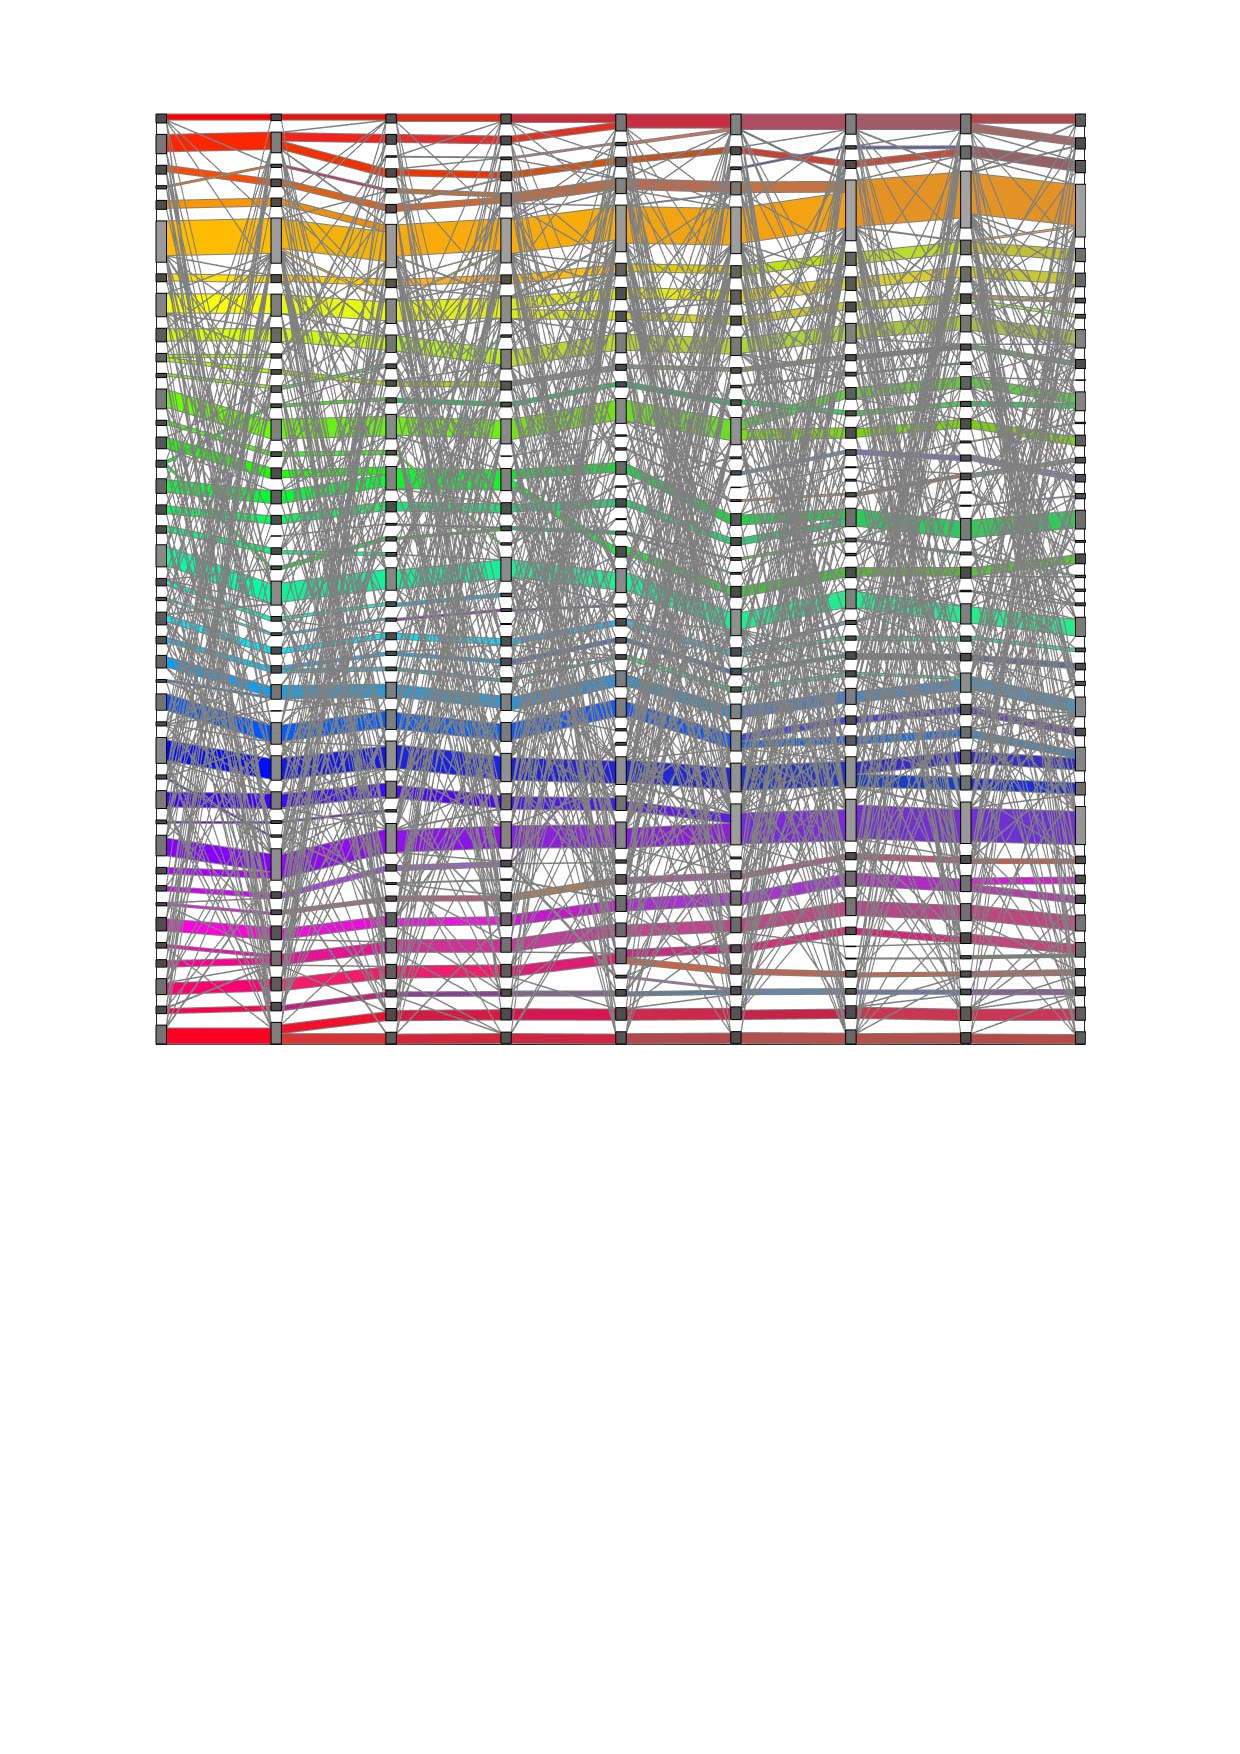
\includegraphics[width=.24\textwidth,height=.15\textwidth]{figures/chap03/dsbm/ASONEMmsEvolution/1HBDSBM.pdf}
	}
	\subfigure[GenLouvain]{
		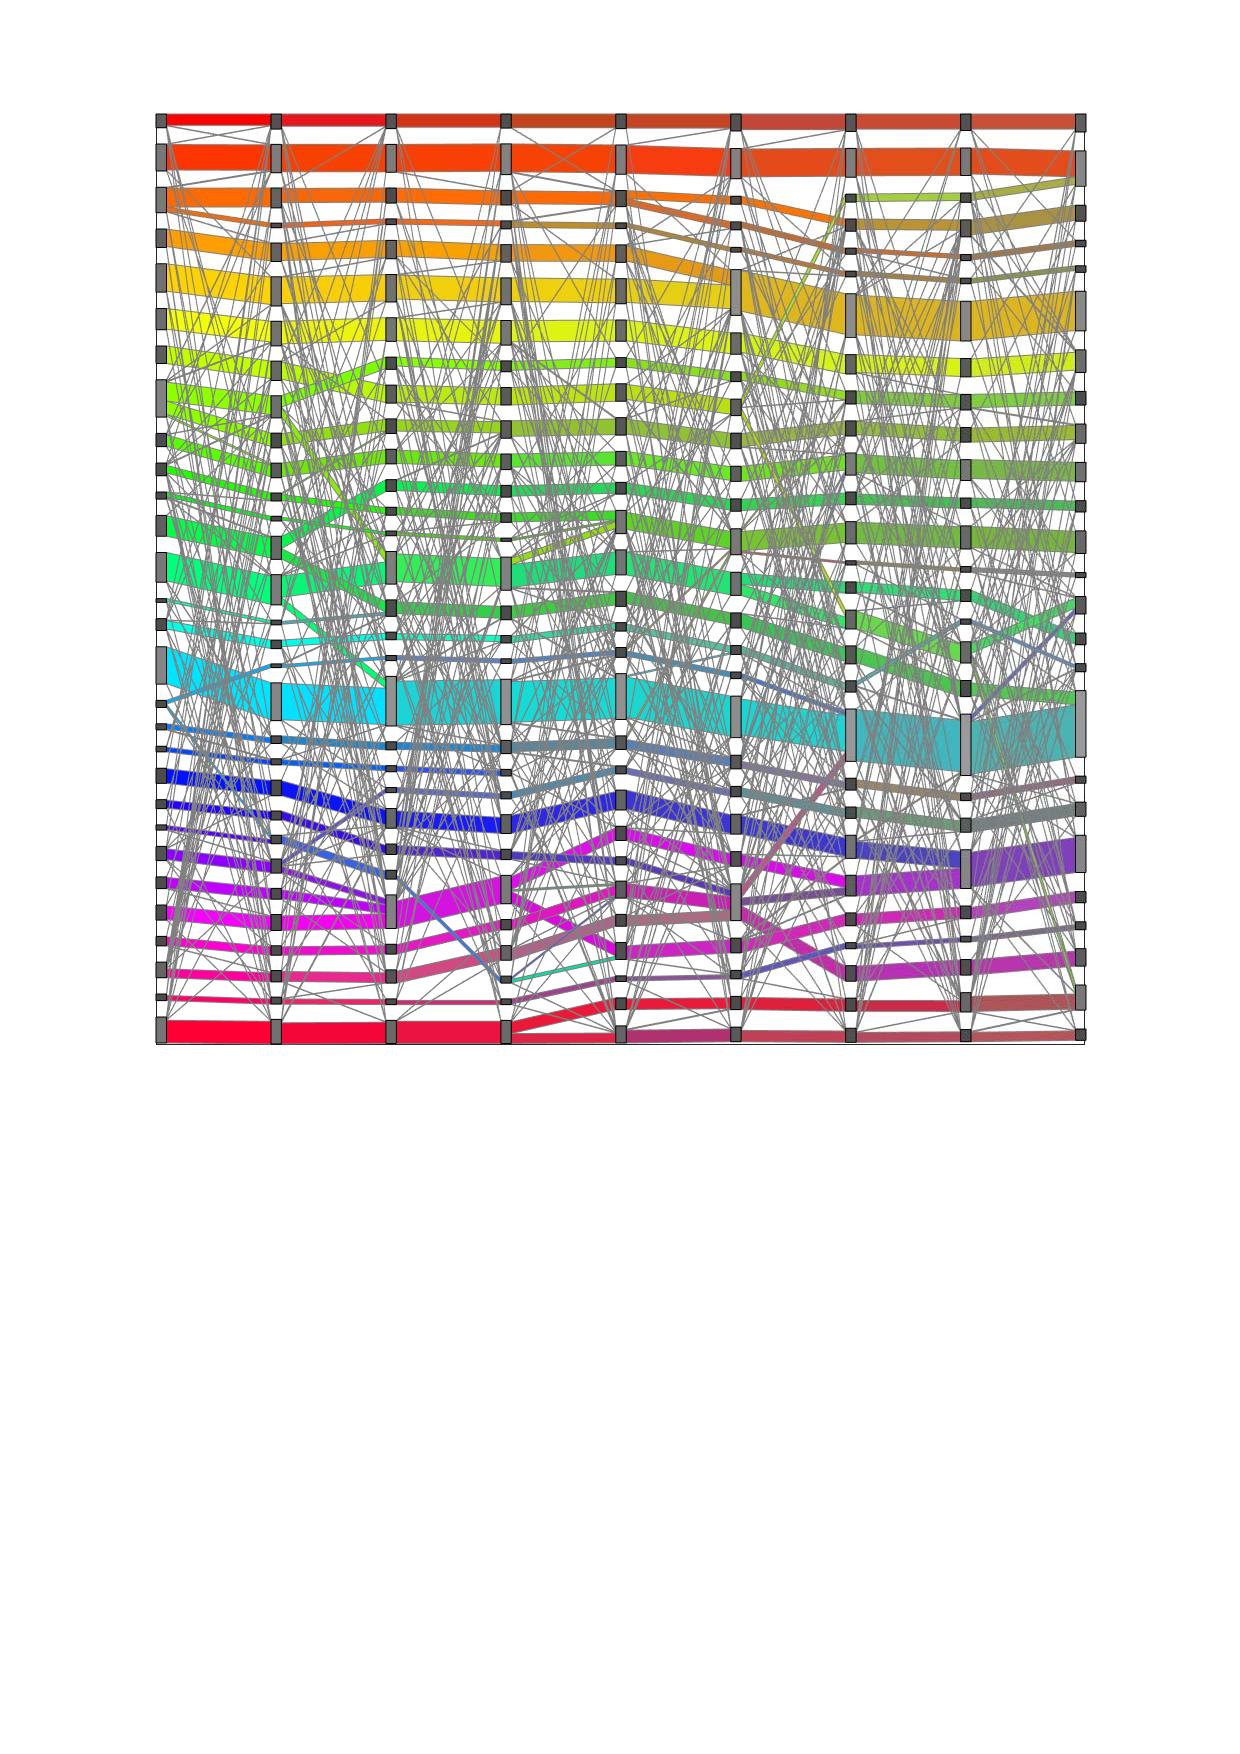
\includegraphics[width=.24\textwidth,height=.15\textwidth]{figures/chap03/dsbm/ASONEMmsEvolution/1gen.pdf}
	}
	\subfigure[PisCES]{
		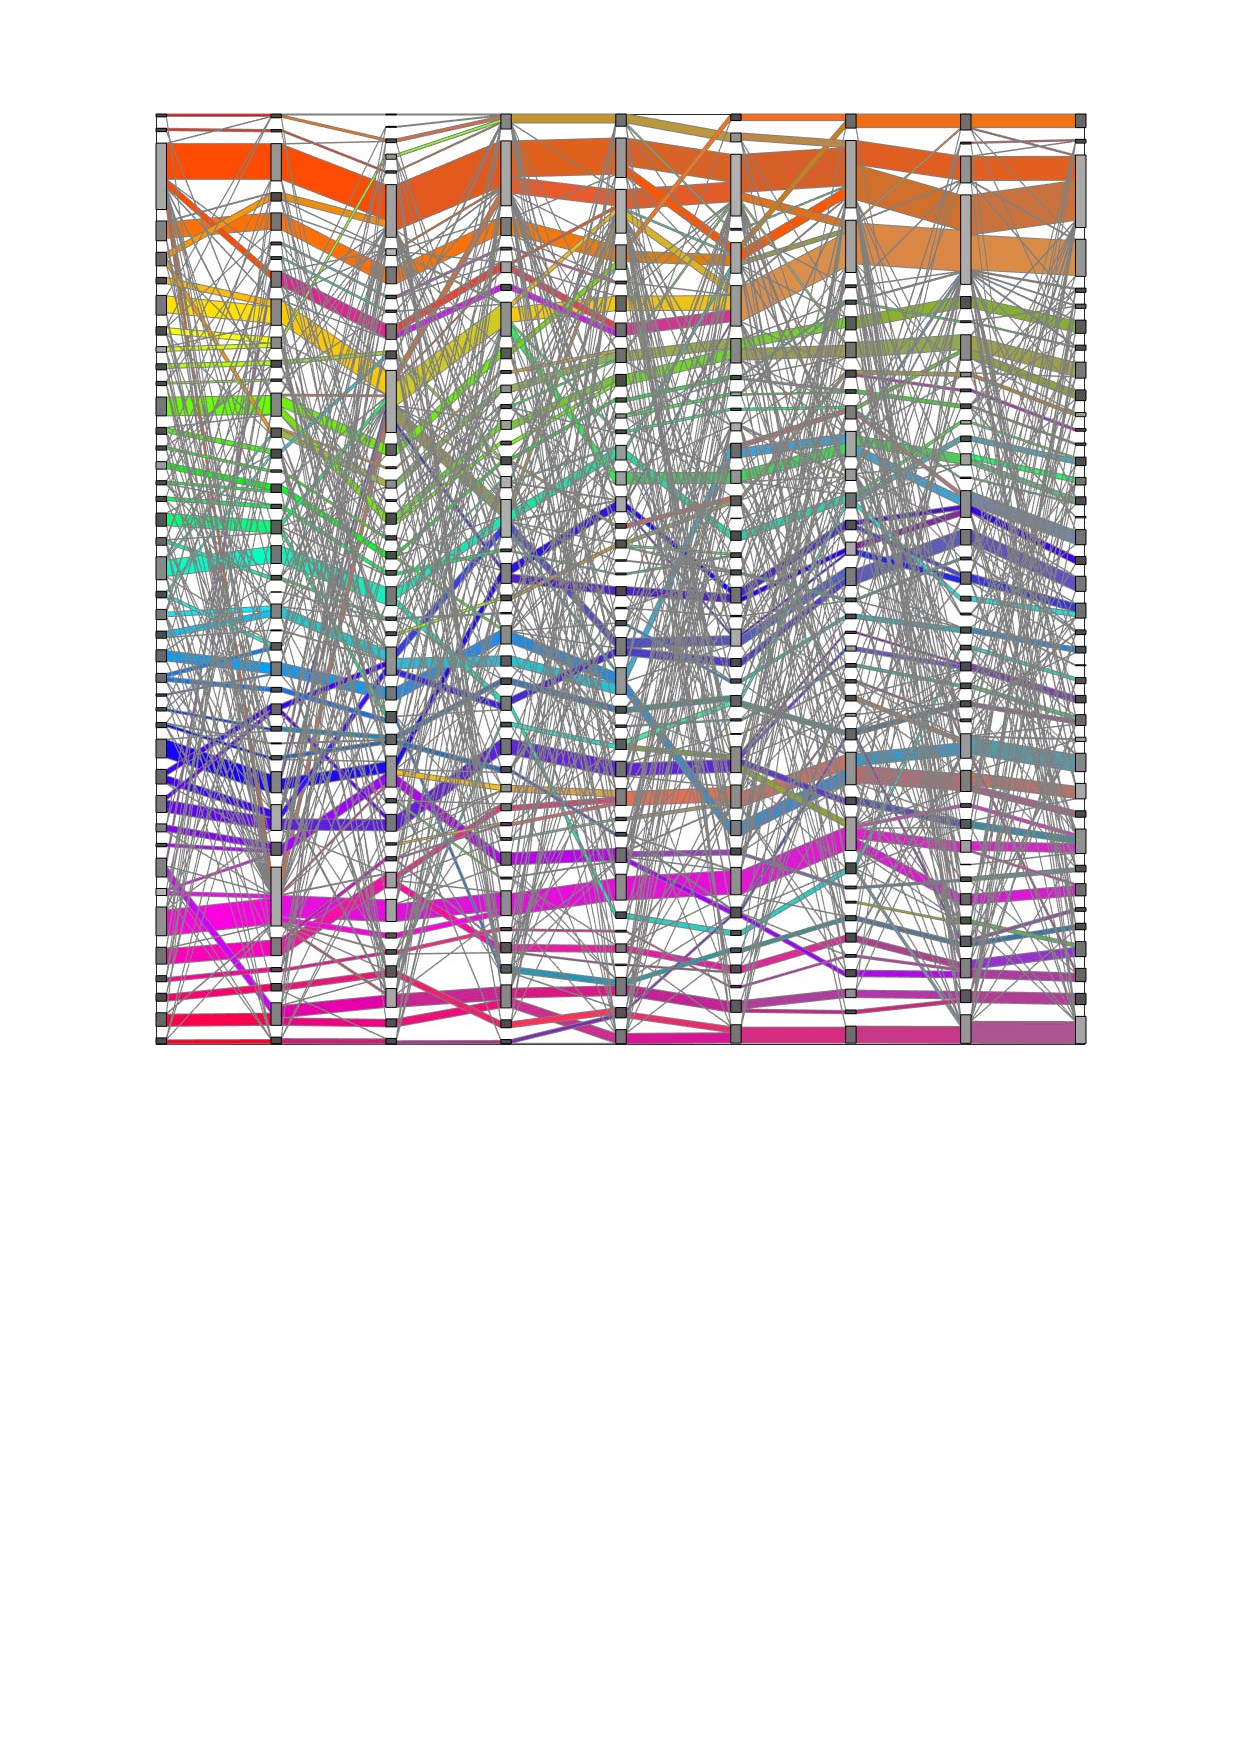
\includegraphics[width=.24\textwidth,height=.15\textwidth]{figures/chap03/dsbm/ASONEMmsEvolution/1PisCES.pdf}
	}
	\subfigure[DYNMOGA]{
		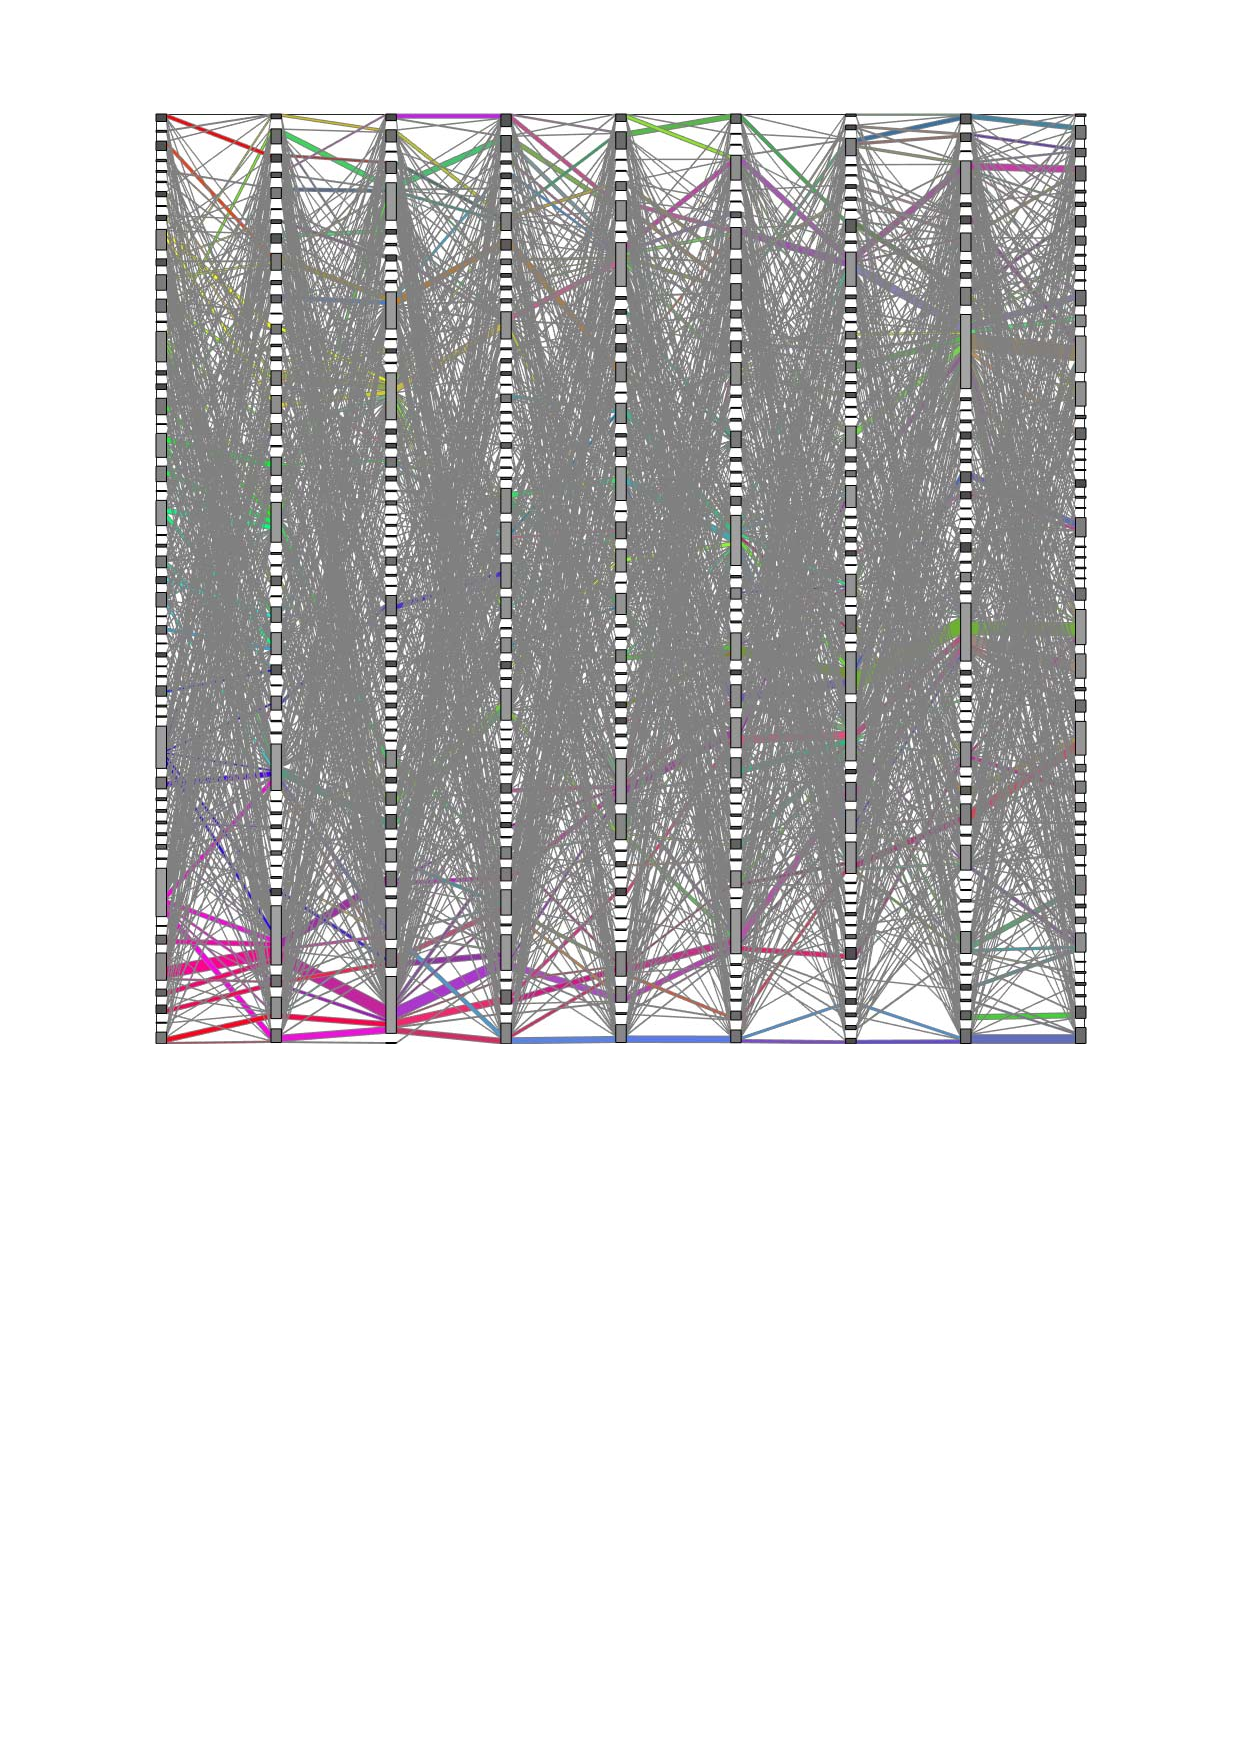
\includegraphics[width=.24\textwidth,height=.15\textwidth]{figures/chap03/dsbm/ASONEMmsEvolution/1dynmoga.pdf}
	}
	\caption{生成数据2中社团分裂合并事件数据的社团演化桑基图}
	\label{fig:SankeyAsonamMS}
	  \vspace{-0.5cm}
\end{figure}



另外,本节还分析了HB-DSBM的社团转移矩阵$A$的实际意义,如图~\ref{fig:block}所示,热图中颜色越浅表示转移倾向越高。可以看到HB-DSBM的社团转移矩阵符合社团的定义,同时所建模的节点转移异质性也起到了有效作用,节点更倾向于在时序过程中保留在本社团内,但保留了转移到其他社团的倾向,而DSBM则更加极端。PisCES对社团转移的倾向刻画则更加混乱。

\begin{figure}
	\centering
	\subfigure[GroundTruth]{
		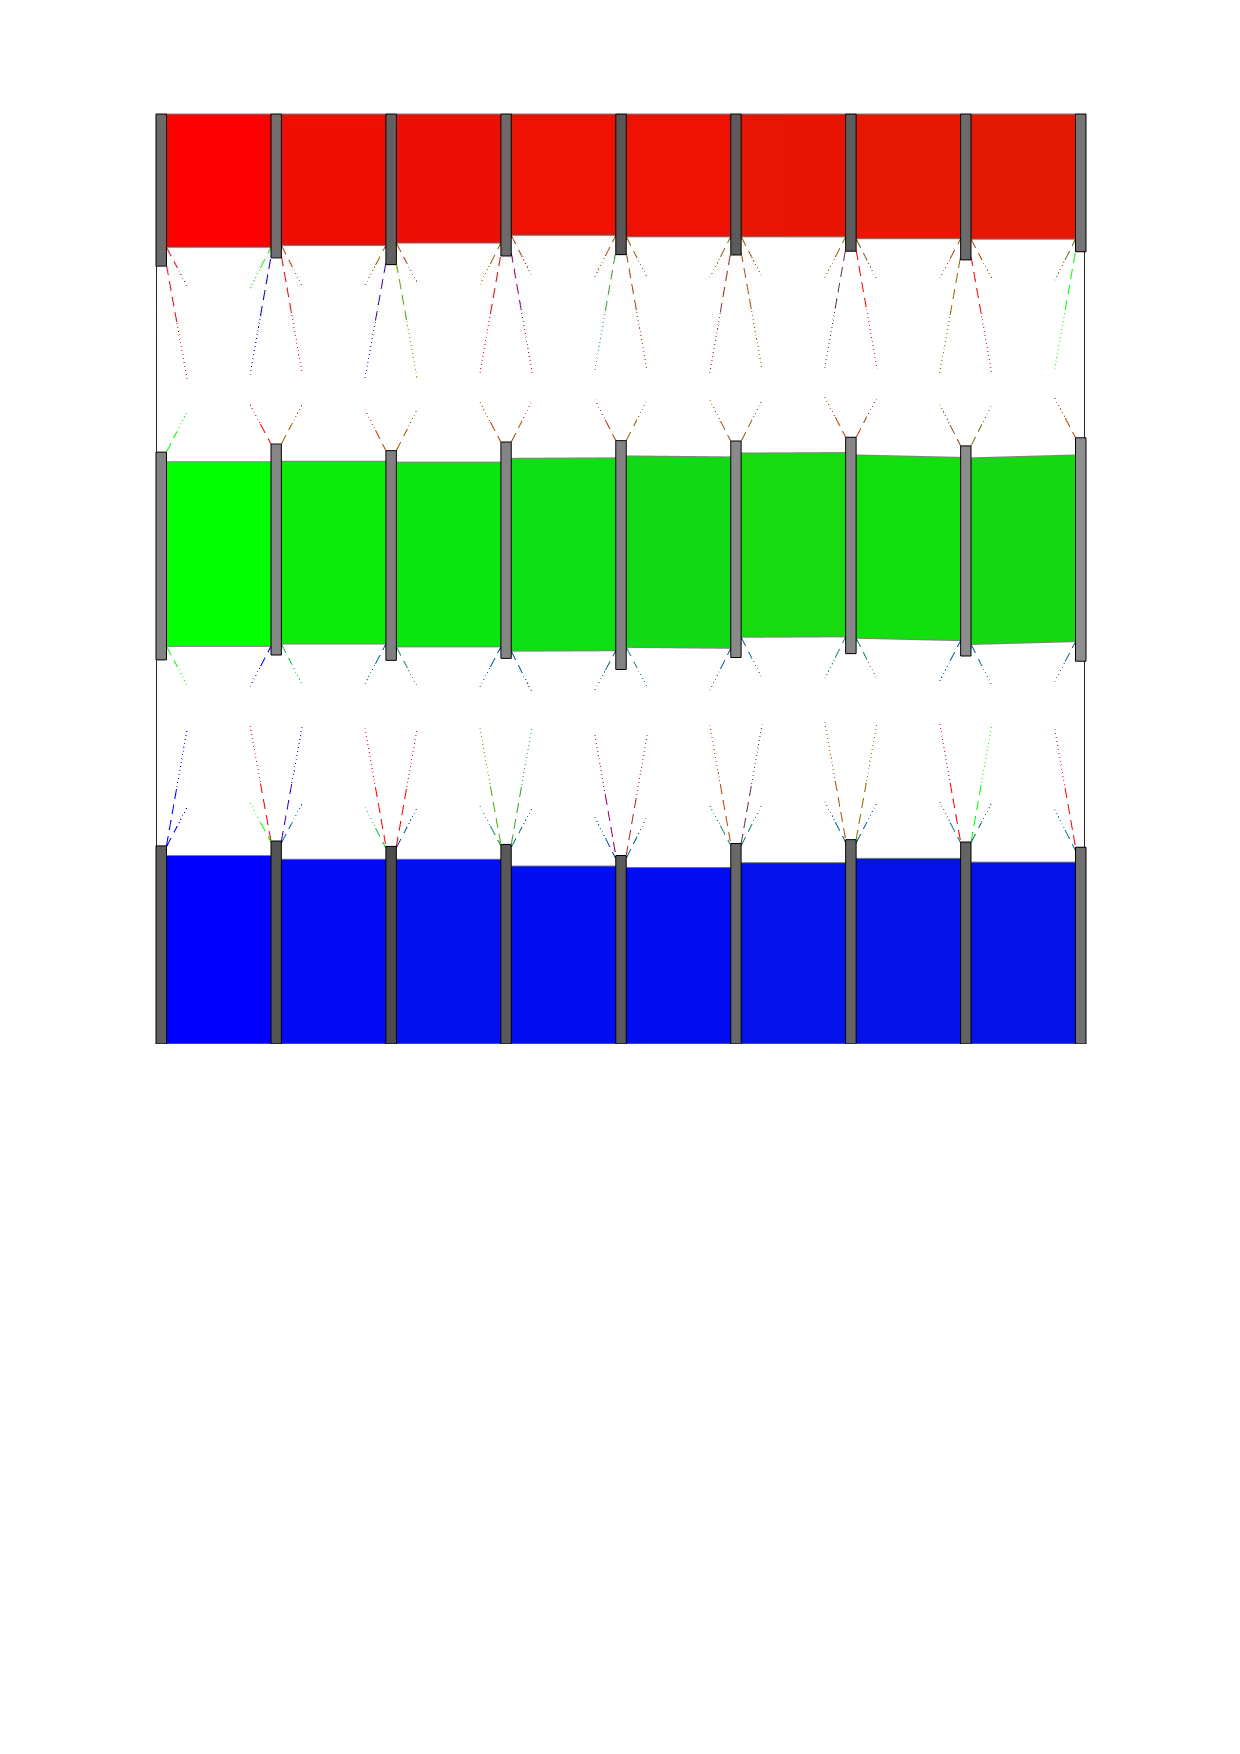
\includegraphics[width=.24\textwidth,height=.1\textwidth]{figures/chap03/dsbm/dblpEvolution/GroundTruth.pdf}
	}
	\subfigure[DSBM]{
		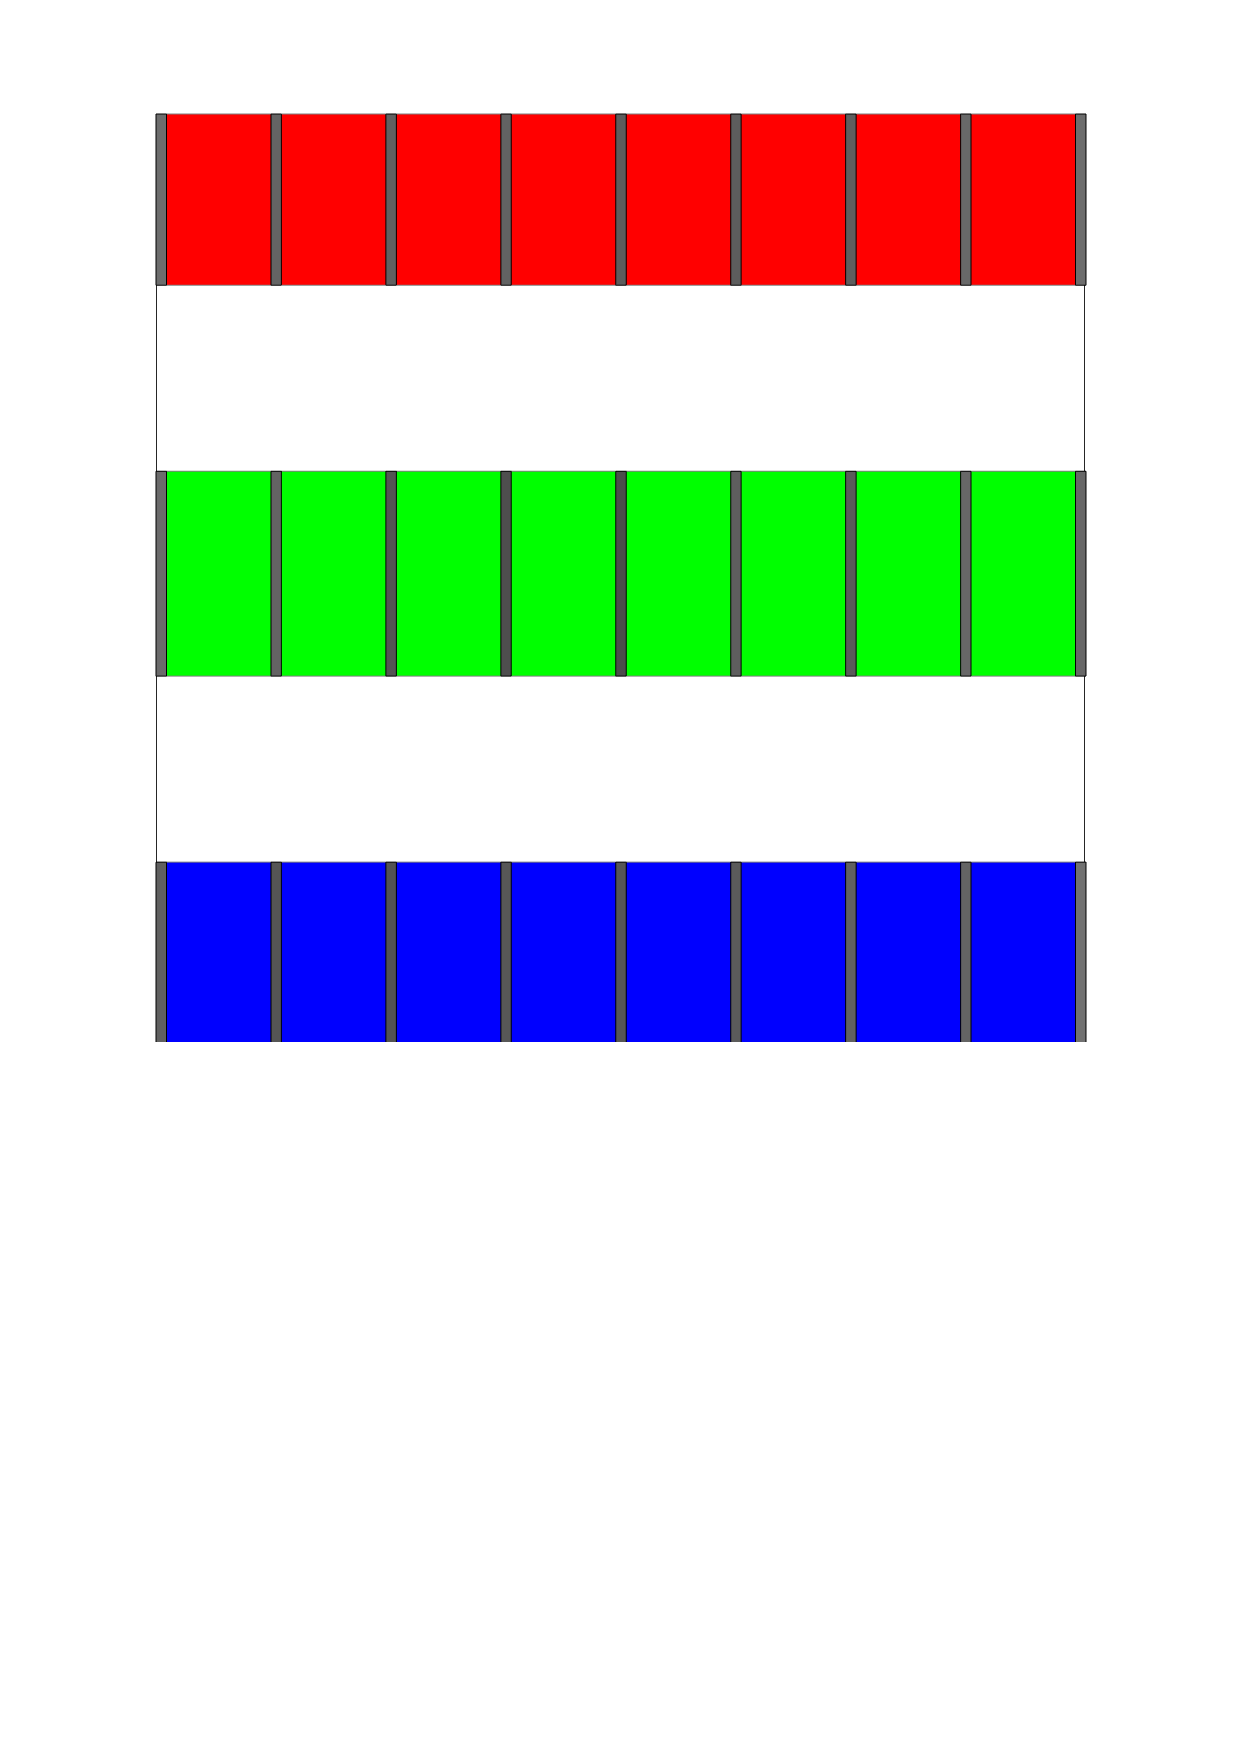
\includegraphics[width=.24\textwidth,height=.1\textwidth]{figures/chap03/dsbm/dblpEvolution/DSBM.pdf}
	}
	\subfigure[HB-DSBM]{
		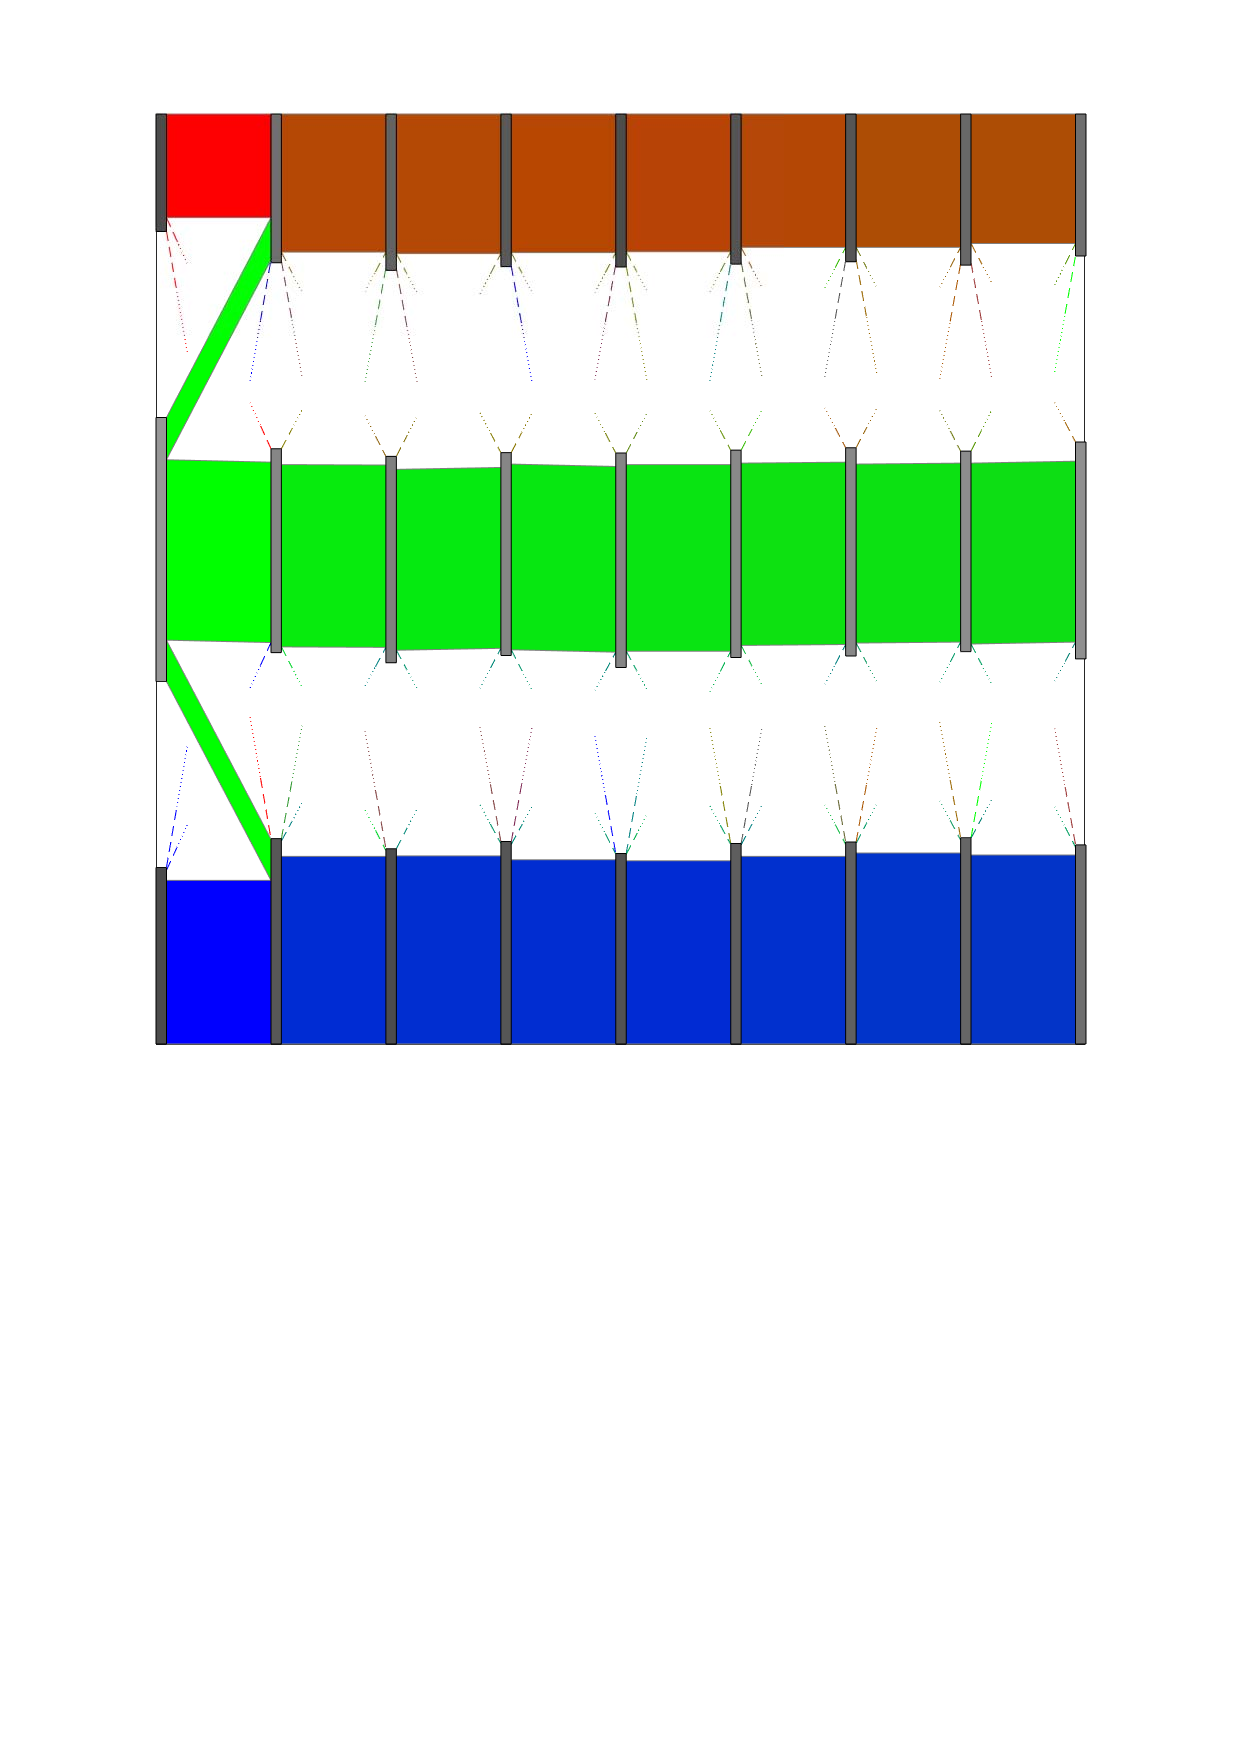
\includegraphics[width=.24\textwidth,height=.1\textwidth]{figures/chap03/dsbm/dblpEvolution/HB-DSBM.pdf}
	}
	\subfigure[GenLouvain]{
		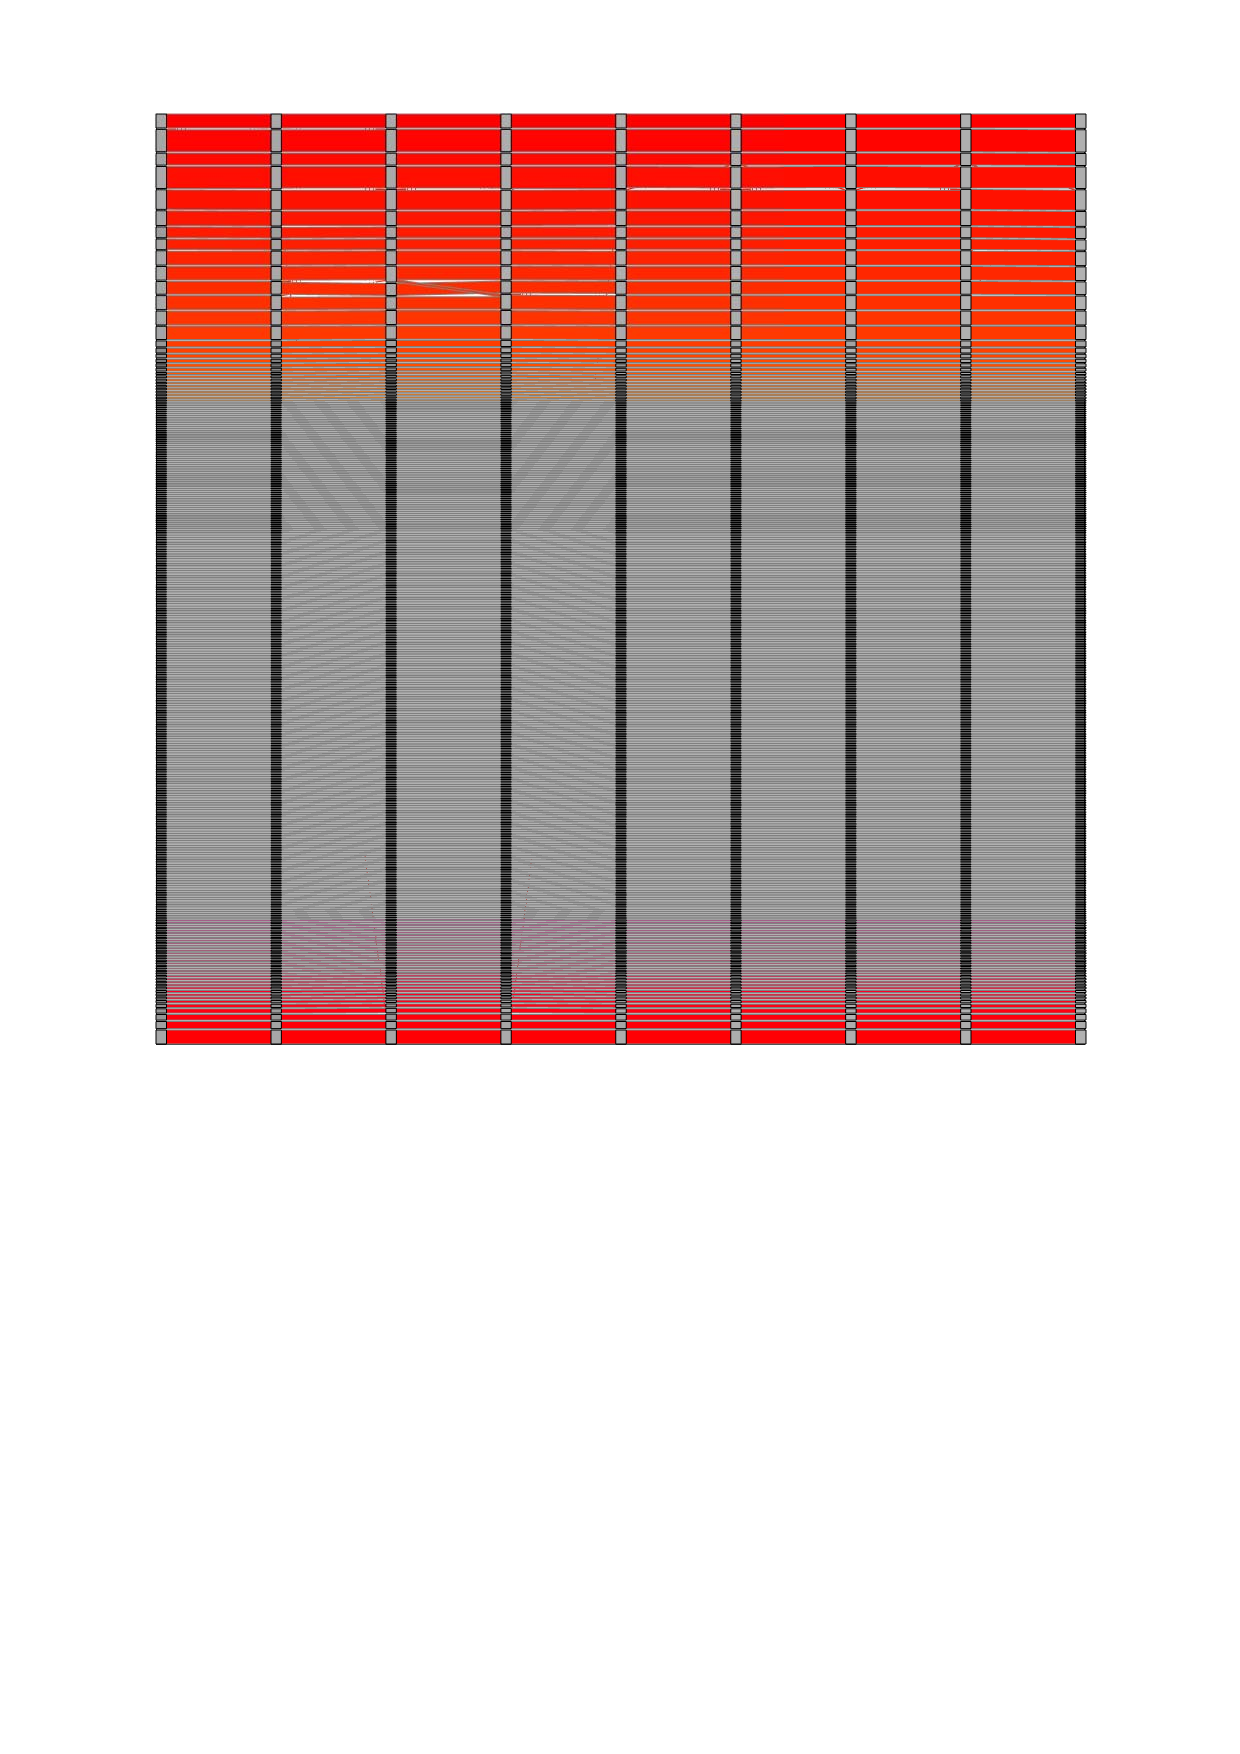
\includegraphics[width=.24\textwidth,height=.1\textwidth]{figures/chap03/dsbm/dblpEvolution/gen.pdf}
	}
	\subfigure[PisCES]{
		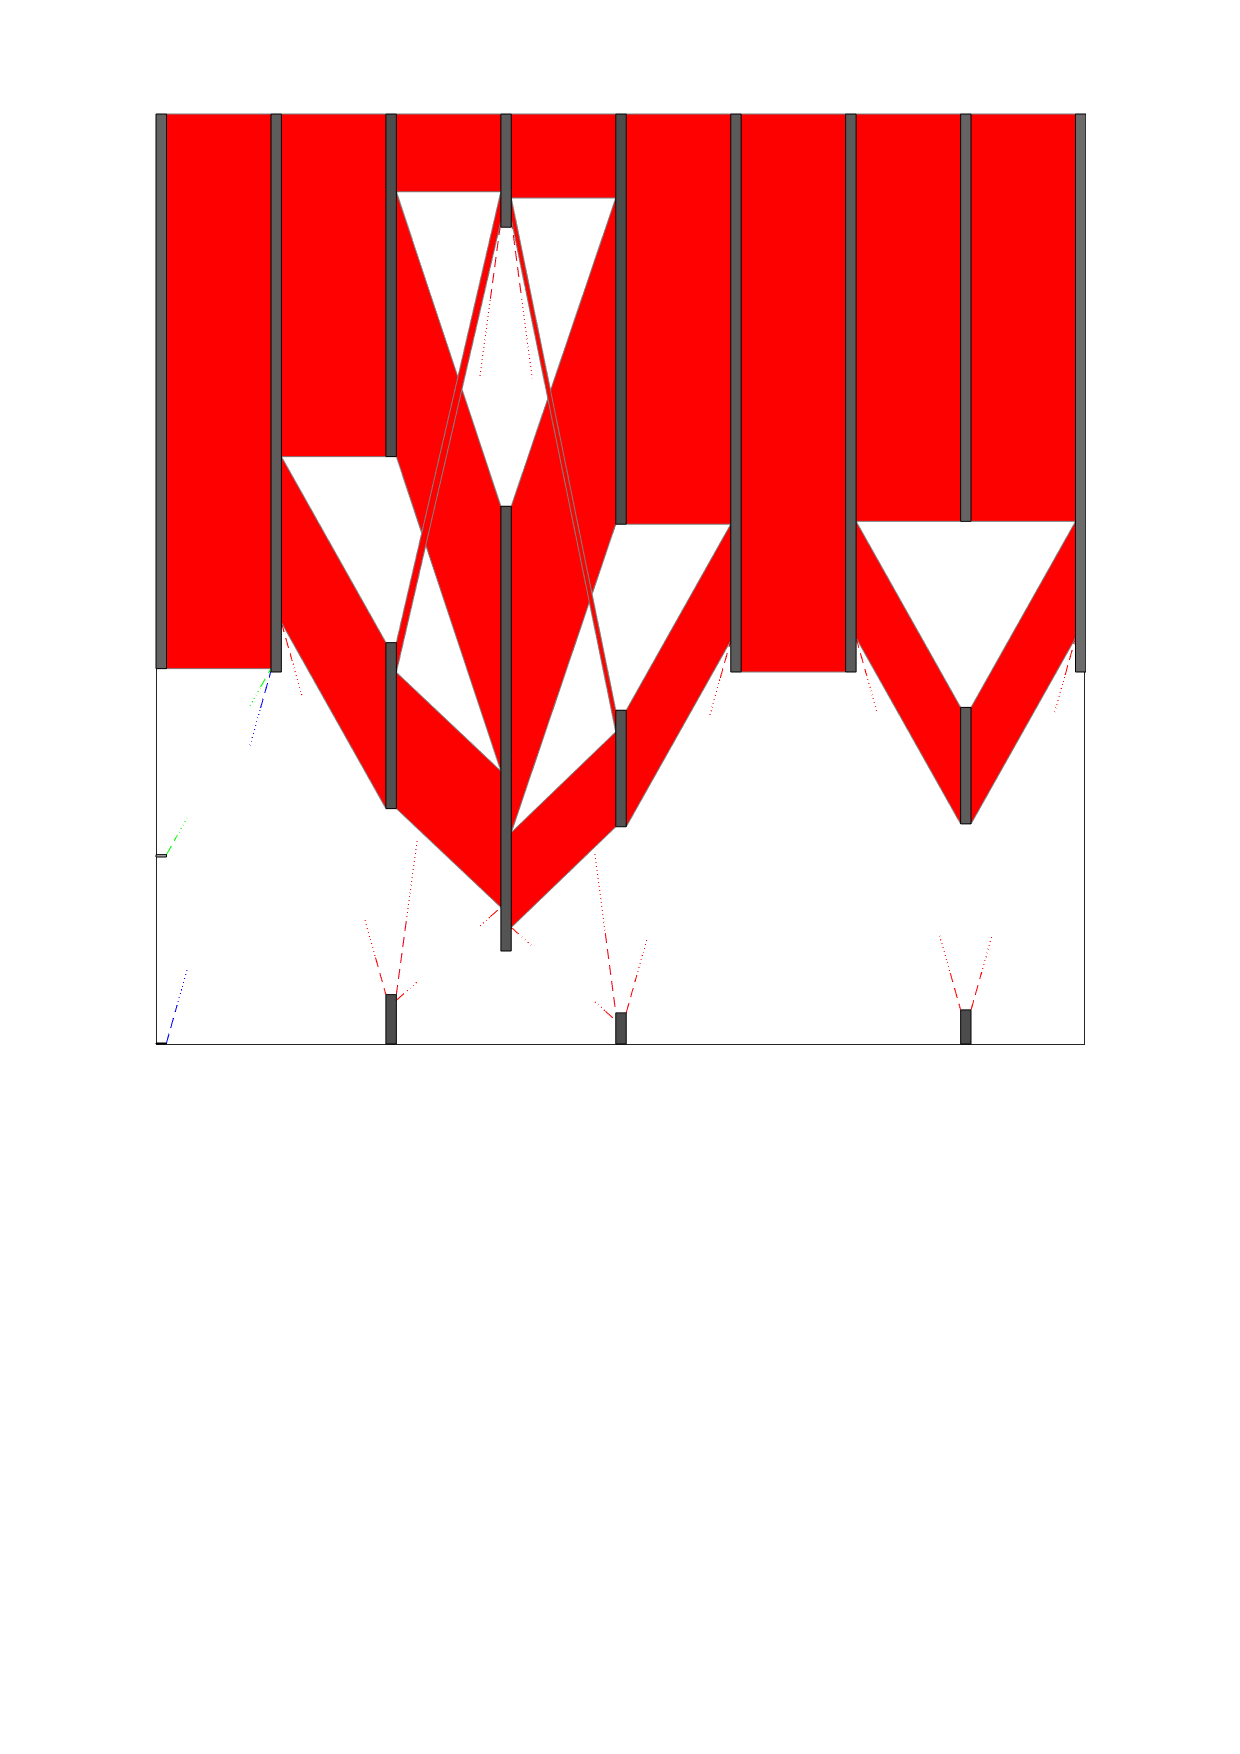
\includegraphics[width=.24\textwidth,height=.1\textwidth]{figures/chap03/dsbm/dblpEvolution/PisCES.pdf}
	}
	\subfigure[DYNMOGA]{
		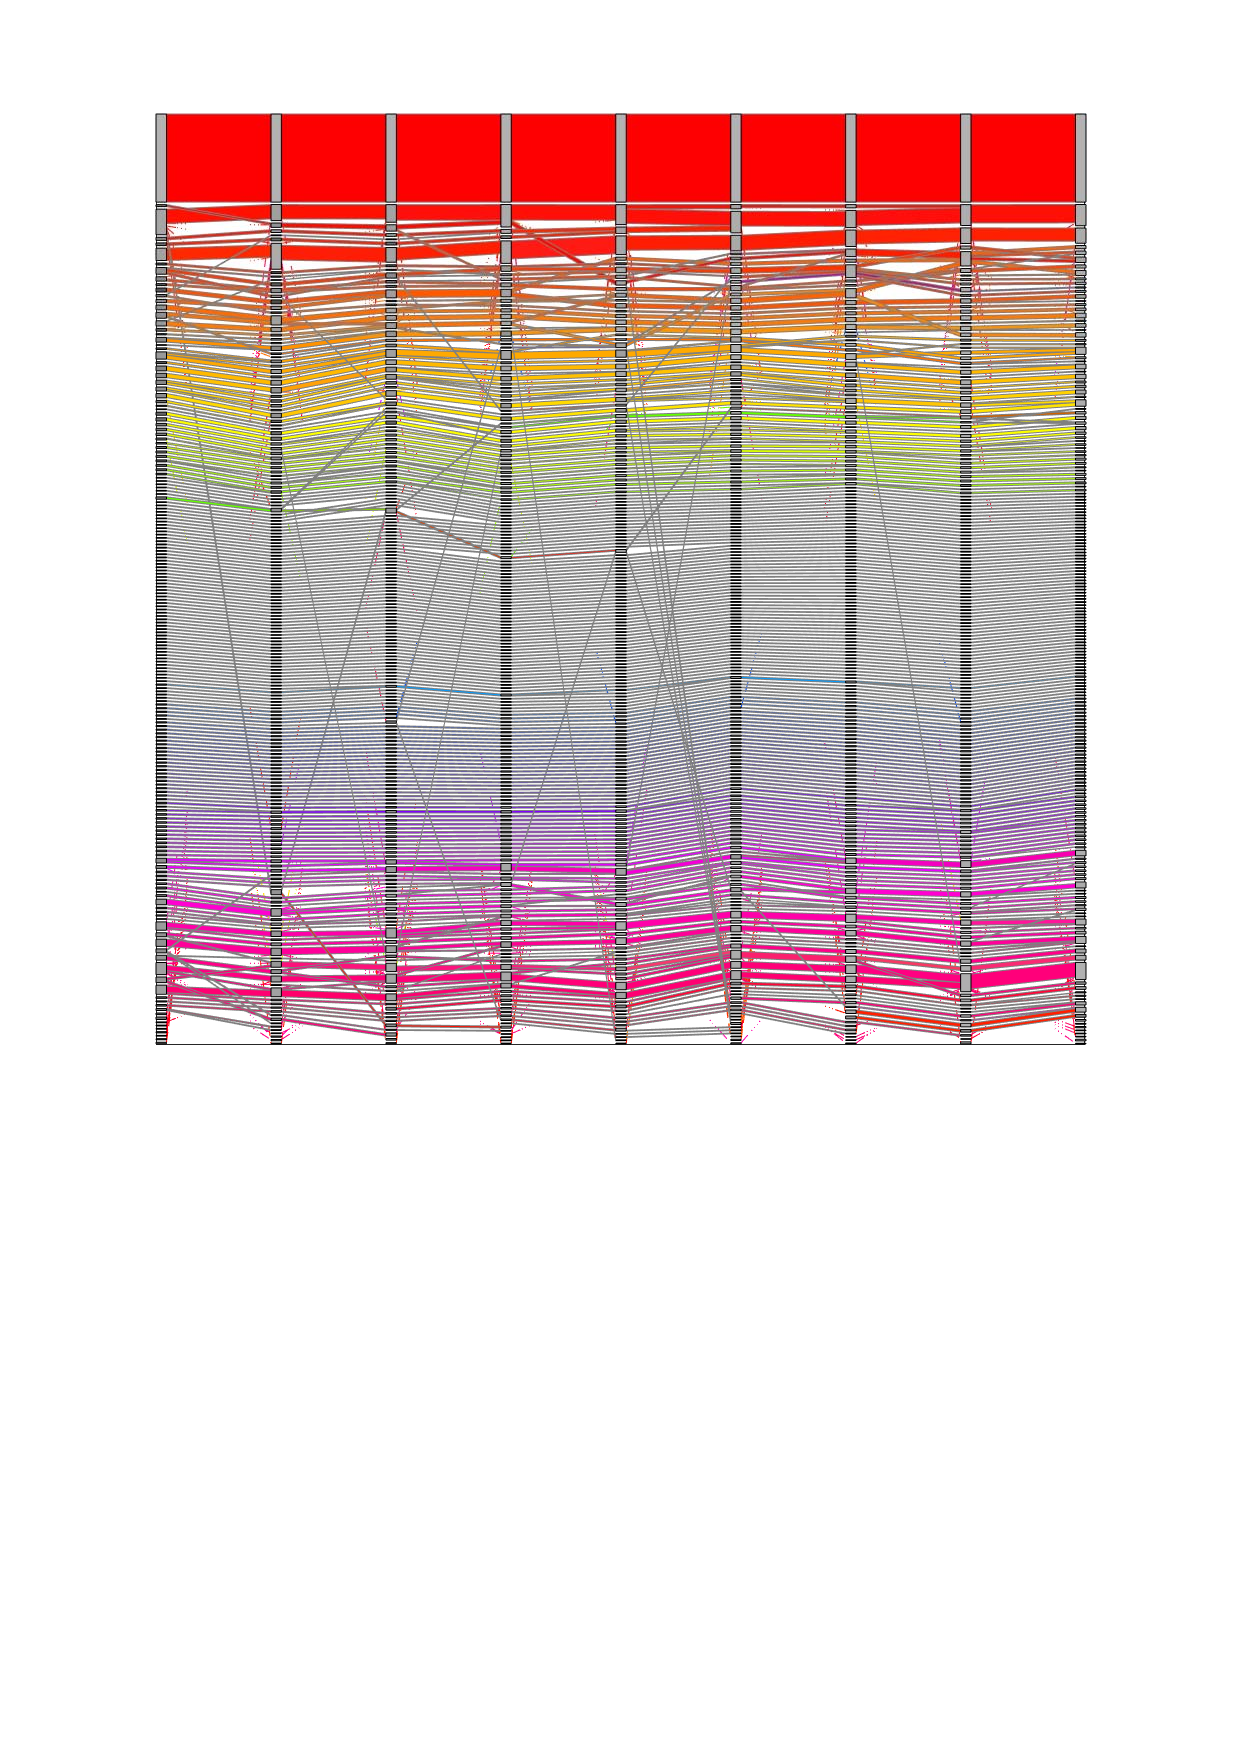
\includegraphics[width=.24\textwidth,height=.1\textwidth]{figures/chap03/dsbm/dblpEvolution/dynmoga.pdf}
	}
	\caption{DBLP数据的社团演化桑基图}
	\label{fig:SankeyDBLP}
	\vspace{0cm}
\end{figure}

\begin{figure}
\centering
\subfigure[DBLP]{
	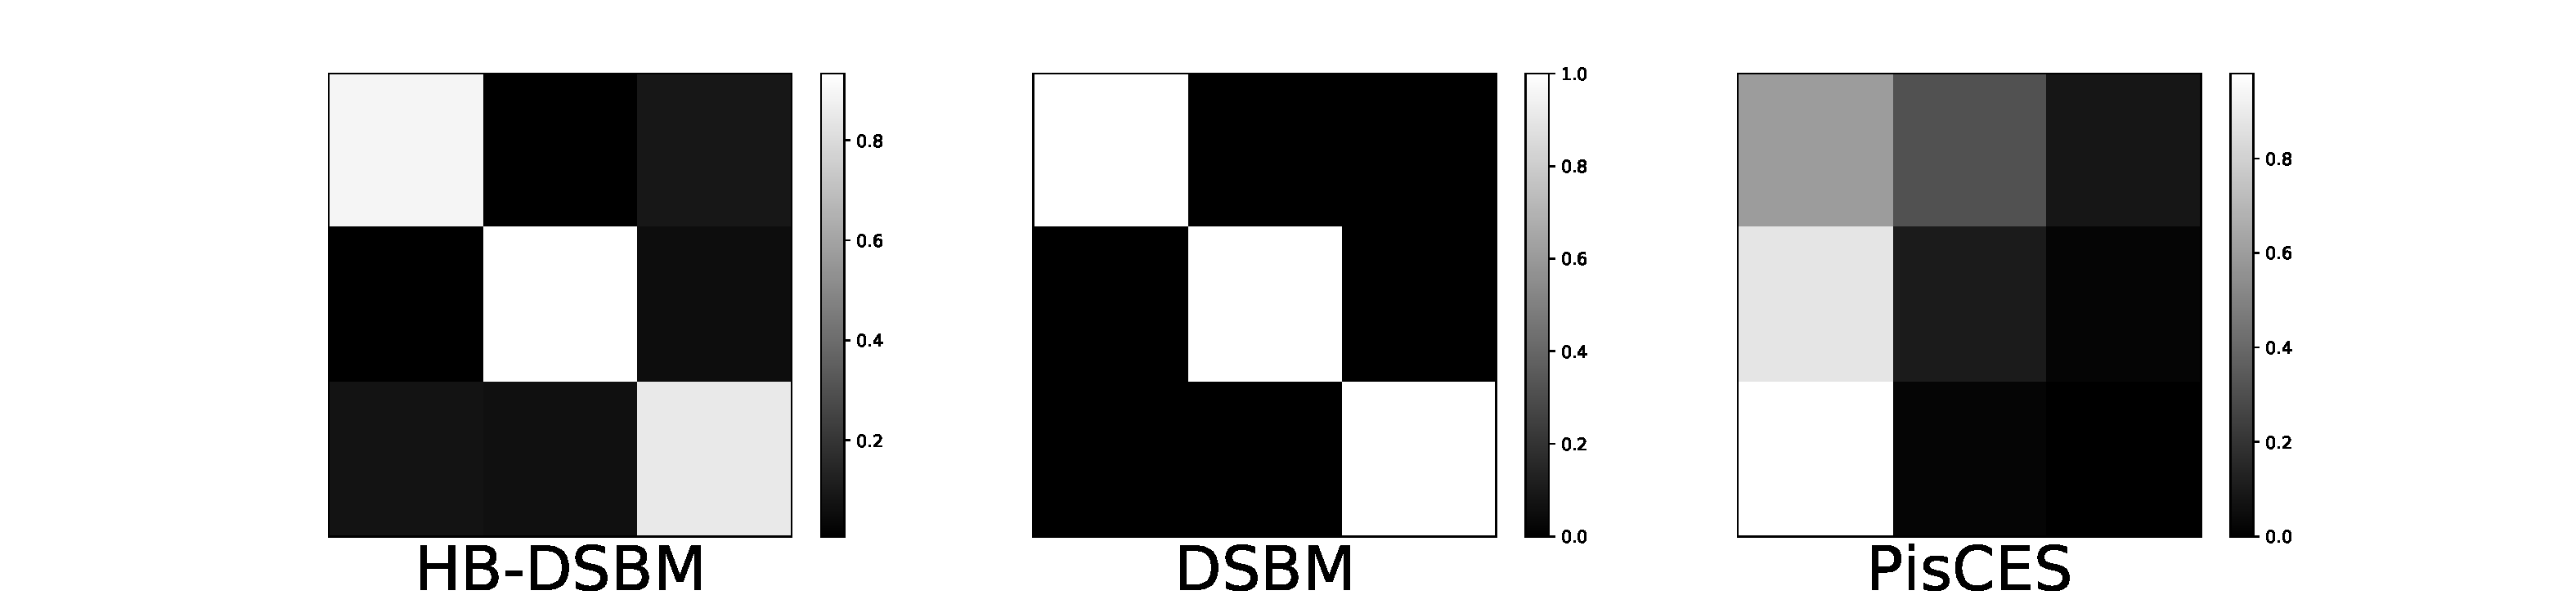
\includegraphics[width=.46\textwidth]{figures/chap03/dsbm/blockMatrixVis/dblpcommunityHeatMap3.pdf}
}
\;\;\;\;
\subfigure[生成数据$2$分裂合并数据]{
	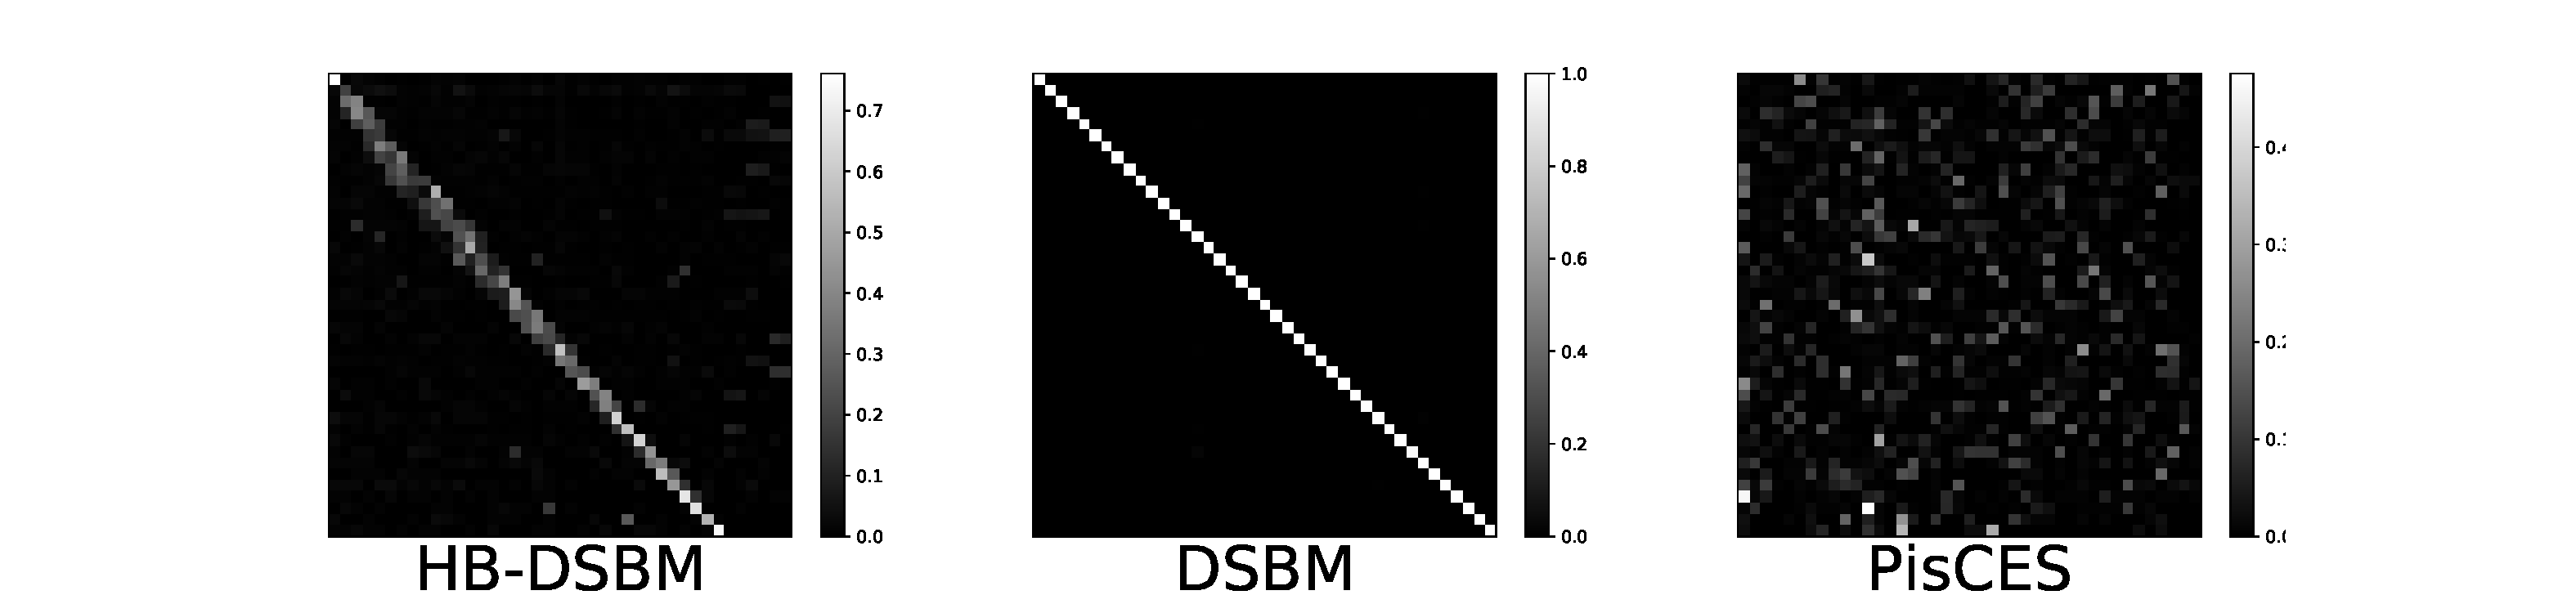
\includegraphics[width=.46\textwidth]{figures/chap03/dsbm/blockMatrixVis/ASONMScommunityHeatMap3.pdf}
}
% \subfigure[FacetNet $\sigma = 5$, $nC = 9$, and $aD = 20$ ]{
	% 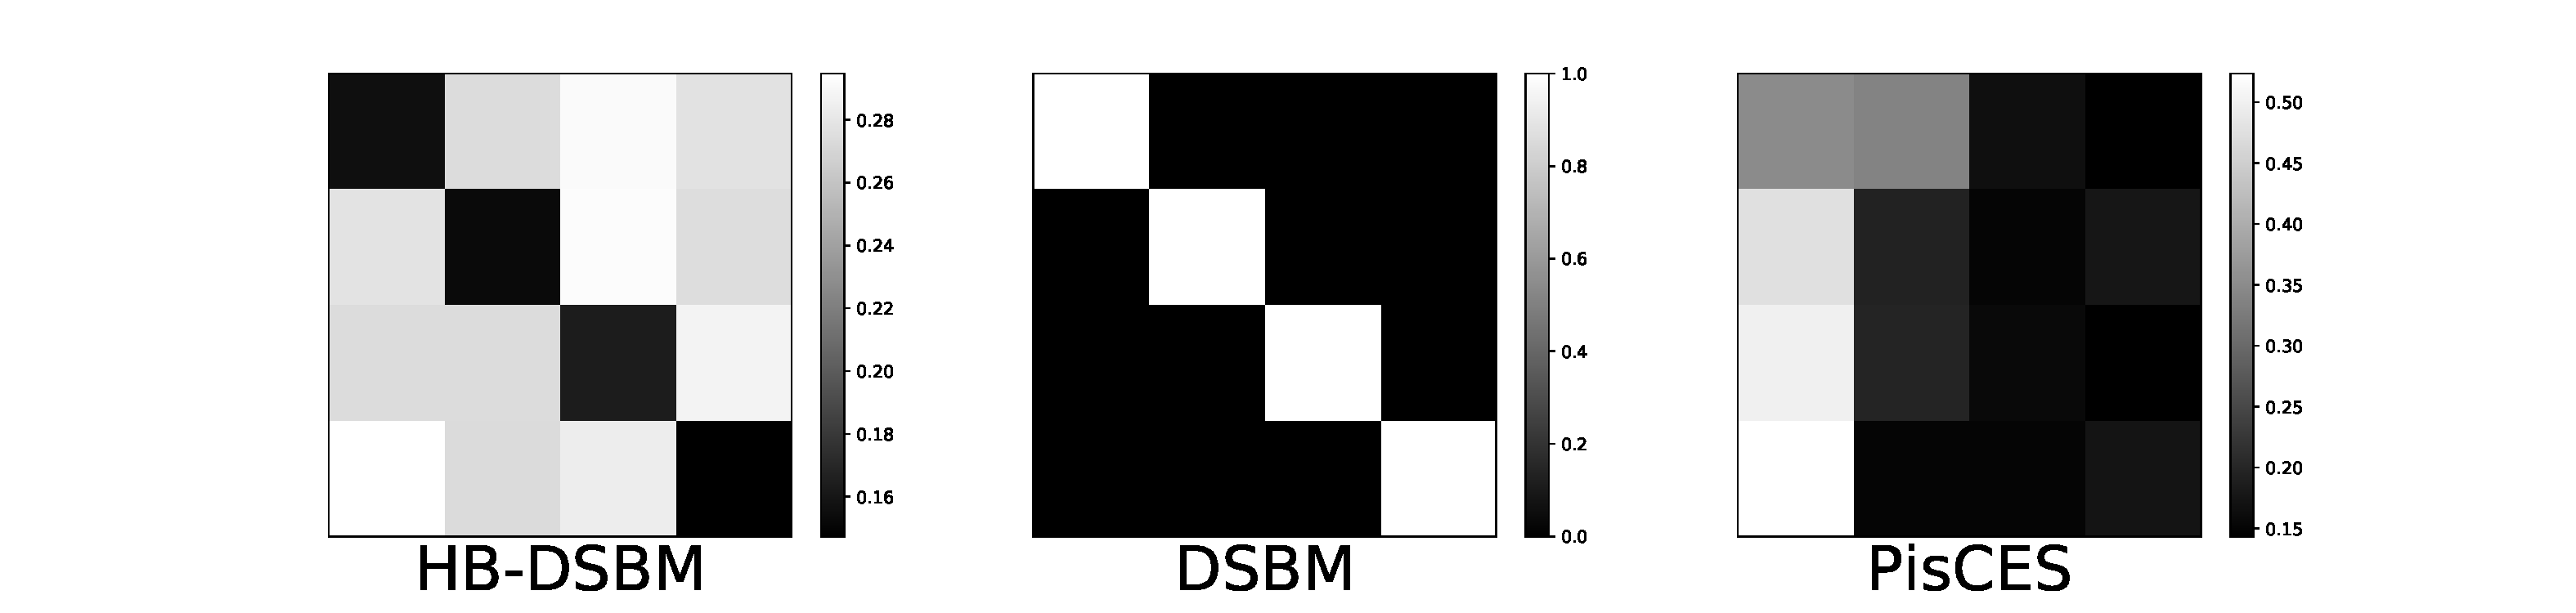
\includegraphics[width=.48\textwidth]{pictures/blockMatrixVis/facetNet5920communityHeatMap3.pdf}
	% }
\caption{社团转移矩阵$A$的热图可视化}% Notice that only DSBM, HB-DSBM and PisCES have `block matrix'. }
\label{fig:block}
%\vspace{-0.5cm}
\end{figure}

\subsection{节点的演化异常分析}
另外,为了验证节点及转移参数$C$的实际意义与有效性,本章根据$C$对节点演化异质性的概念,提出了节点演化异常的定义,即在动态网络中存在频繁变换其社团归属的节点,并利用熵对节点$i$的演化异常指数进行定义:
\begin{equation}
	E_i = -\sum_{t=1}^{T-1} \sum_{k} C_{tik} \log C_{(t+1)ik},
	\label{Nodeanomaly3}
\end{equation}
$E_i$越大,表示节点$i$的演化越频繁,则认为其是异常节点。如图~\ref{fig:anomalyPics}所示,在DBLP数据中,$E_i$较高的节点较少,整体呈现出较稳定的趋势,证明DBLP数据中,研究人员的研究领域相对稳定,这由图~\ref{fig:SankeyDBLP}可以进行佐证。而专利数据Patent则呈现出了剧烈的节点变动,证明在计算机领域的专利合作并不像论文合作一样稳定,从直观上来看,专利的发表更关注第一发明人,其余发明人的权重在我国并不高,这也验证了该结论。而针对生成数据2中社团分裂合并数据的测试则验证了所定义的节点异常指数的有效性。


\begin{figure}
	\centering
	\subfigure[DBLP]{
		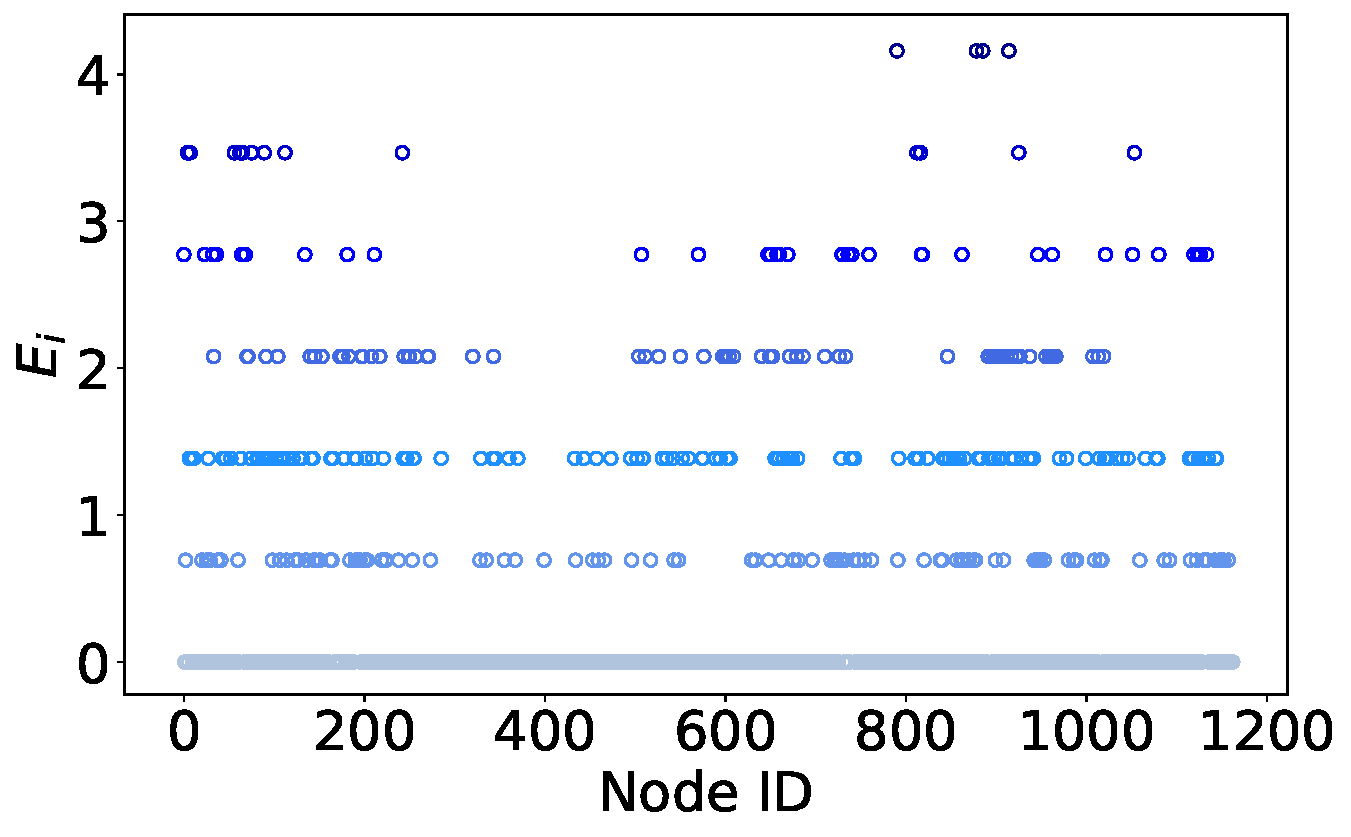
\includegraphics[width=.3\textwidth]{figures/chap03/dsbm/anomaly/dblpAnomalyPic6.pdf}
	}
	\subfigure[Patent]{
		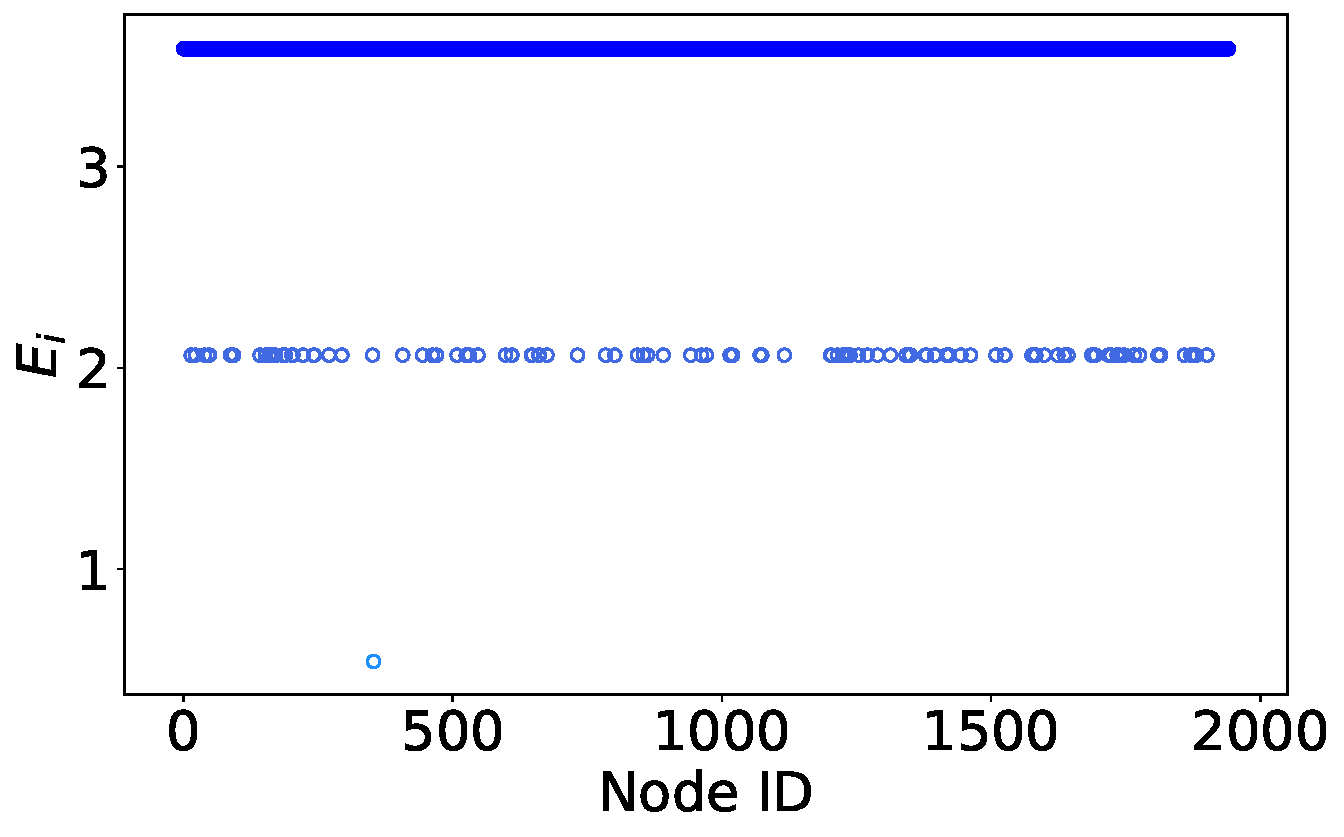
\includegraphics[width=.3\textwidth]{figures/chap03/dsbm/anomaly/patentAnomalyPic6.pdf}
	}
	\subfigure[生成数据2分裂合并数据]{
		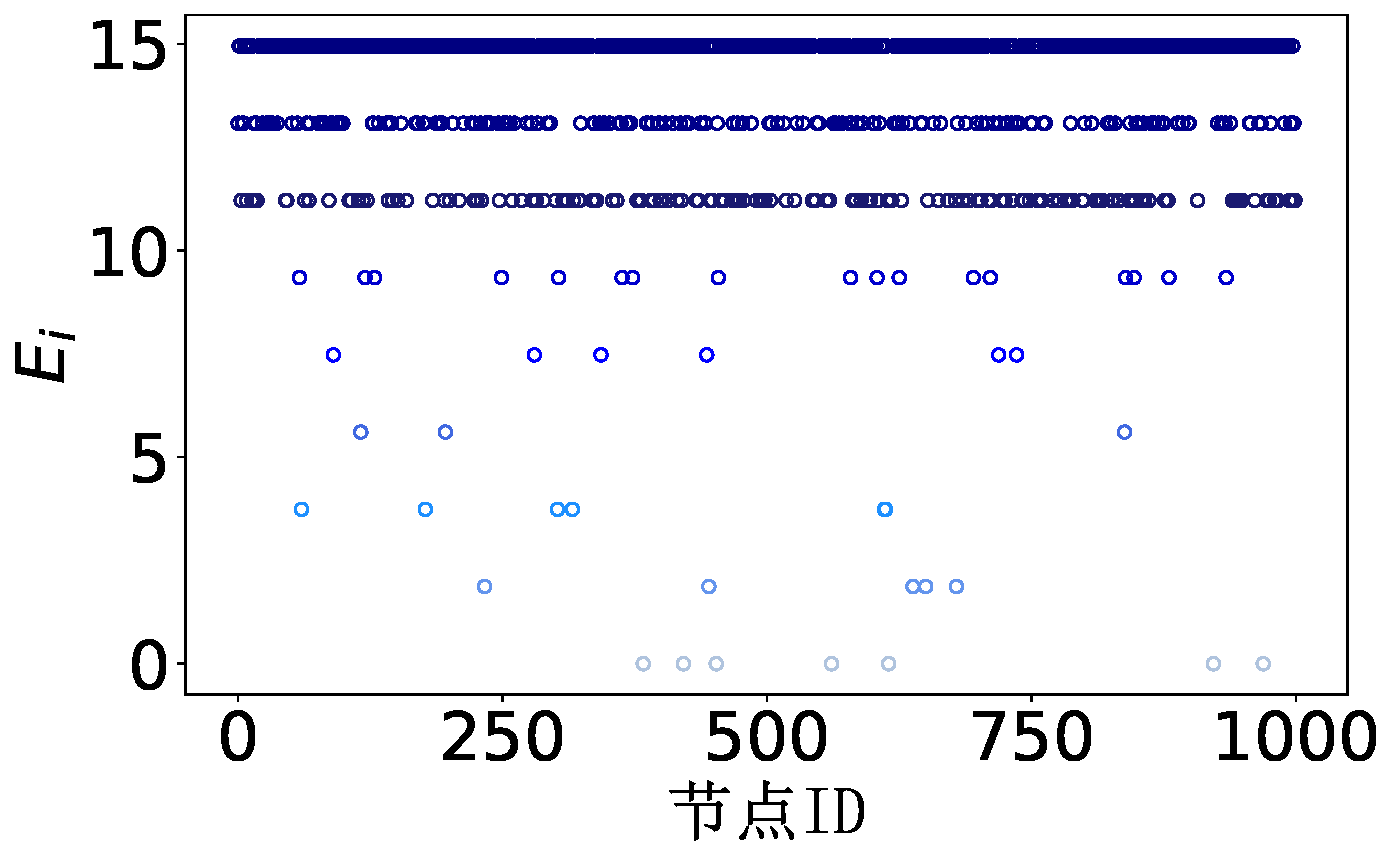
\includegraphics[width=.3\textwidth]{figures/chap03/dsbm/anomaly/msAnomalyPic6.pdf}
	} 
	\caption{基于节点级转移参数$C$的节点演化异常点可视化图}
	\label{fig:anomalyPics}
	%   \vspace{-0.5cm}
\end{figure}


\section{本章小结}
本章首先从实际出发,通过创新性地将节点在动态网络的社团转移倾向异质性挖掘问题转化为节点的社团转移与否的二分类问题,对$15$个各类真实世界动态网络数据进行了实证分析,进而得出结论,动态网络中,节点的社团转移存在异质性,且与节点的度具有较高关联性。根据上述结论,本章进一步基于动态随机块模型设计了层次贝叶斯动态随机块模型,其层次贝叶斯生成结构能够在刻画动态社团演化模式时同时建模节点的社团转移异质性。另外针对所提出的HB-DSBM模型,利用变分推断对模型参数的更新进行了详细的推断,利用合理的优化策略,模型具备适应大规模数据计算的潜力。同类方法的对比也显示出HB-DSBM在动态网络社团检测以及社团演化分析任务中更加高效准确。另外,本文提出的基于节点转移异质性参数提出的节点演化异常指数也在实际分析中得以验证其有效性。

然而从模型设计的角度来看,HB-DSBM仍然存在一定缺陷,首先,其对节点的社团转移异质性建模主要从生成角度而进行的设计,即假设节点的社团转移异质性与社团级别的节点转移倾向有关。具体来说,节点的社团转移异质性服从以其社团级别社团转移倾向为参数的狄利克雷分布。该设计虽然合理,但该参数并未与动态网络中的节点属性直接关联,因此在实际的下游任务中无法直接用于解释不通节点的社团转移倾向;其次,生成模型的优势之一是对于多种下游任务的适配,而所提出的节点演化异常指数还有进一步挖掘其能力的可能。因此,后续章节将针对HB-DSBM中存在的上述问题进行改进。











